\documentclass[a4paper,12pt]{article}
\usepackage{fontspec}
\usepackage{xeCJK}
\setmainfont{Times New Roman}
\usepackage[english]{babel}
\usepackage{amsmath}
\usepackage{amsthm}
\usepackage{amsfonts}
\usepackage{amssymb}
\usepackage{graphicx}
\usepackage{hyperref}
\usepackage{enumitem}
\usepackage{textcomp}
\usepackage{float}
\usepackage{booktabs}

\usepackage[colorinlistoftodos]{todonotes}
\usepackage[left=1.50cm, right=1.50cm, top=1.20cm]{geometry}
\linespread{1.5}
\usepackage{algorithm}
\usepackage{algpseudocode}

\usepackage{tikz}
\usepackage[tikz]{mdframed}
\usetikzlibrary{matrix, positioning, fit, arrows, calc, intersections, shapes, shadings, patterns, decorations.markings, chains, scopes, arrows.meta, shapes.geometric}

\usepackage{tikzsymbols}
\usepackage{tikzpeople}
\usepackage{upquote}
\usepackage{listings}
\lstset{upquote=true}
\lstdefinestyle{customc}{
  belowcaptionskip=1\baselineskip,
  breaklines=true,
  frame=L,
  xleftmargin=\parindent,
  language=C++,
  tabsize=2,
  showstringspaces=false,
  basicstyle=\small\ttfamily,
  keywordstyle=\bfseries\color{green!40!black},
  commentstyle=\itshape\color{purple!40!black},
  identifierstyle=\color{blue},
  stringstyle=\color{orange},
}
\mdfdefinestyle{mymdf}{leftmargin=1cm,rightmargin=2cm,%
innerleftmargin=1cm,innerrightmargin=1cm,roundcorner=10pt,backgroundcolor=lg}
\title{Algorithm Problem Set \\ \large No. 001 --- 100}
\author{SS}
\date{November 2018}

\begin{document}
\renewcommand{\thelstlisting}{\thesection.\arabic{lstlisting}}
%\sloppy
\maketitle
%\section{3 --  Longest Substring Without Repeating Characters}
Given a string $S$, find the length of the longest substring without repeating characters.

\paragraph{Example 1:}
\begin{flushleft}
\textbf{Input}: \texttt{abcabcbb}
\\
\textbf{Output}: 3 
\\
\textbf{Explanation}: The answer is \texttt{abc}, with the length of 3. 
\end{flushleft}

\paragraph{Example 2:}
\begin{flushleft}
\textbf{Input:} \texttt{bbbbb}
\\
\textbf{Output}: 1
\\
\textbf{Explanation}: The answer is \texttt{b}, with the length of 1.
\end{flushleft}

\paragraph{Example 3:}

\begin{flushleft}
\textbf{Input}: \texttt{pwwkew}
\\
\textbf{Output}: 3
\\
\textbf{Explanation}:
\\
The answer is \texttt{wke}, with the length of 3. Note that the answer must be a substring, \texttt{pwke} is a subsequence and not a substring.

\end{flushleft}
\subsection{Hash Map}
用一个\texttt{hashmap}来记录每个字符出现的位置,并逐步更新最新的位置。这是因为如果字符\quad $s[j]$ \quad 在 \quad $s[\mathtt{start}\ldots j-1]$ \quad 中在\quad$k$\quad 处重复,那么只需要把\quad$\mathtt{start}$\quad 更新到\quad$k+1$\quad 就可以了。
\begin{algorithm}[H]
\caption{Get longest substring without duplicates}
\begin{algorithmic}[1]
\Procedure{GetLongestSubstring}{$S, L$}
\State \textbf{initialize} an array $M$ with \textbf{256} elements that are set to \textbf{-1}.
\State $p := 0 $
\State $\ell:= 0$ \Comment maximum length initialized to \textbf{zero}
\For{$i := 0$ \textbf{to} $L$}
\If{$M[S(i)] \neq -1$} \Comment found repeat $S(i)$ in $S[p\ldots i-1]$
\State $p \gets \max(p, M[S(i)]) + 1$ \Comment update to the next index of the duplicate
\EndIf
\State $\ell \gets \max(\ell, i - p +1 )$ \Comment update current maximum length
\State $M[S(i)] \gets i$ \Comment update $M[S(i)]$ by latest index
\EndFor
\State \Return $\ell$
\EndProcedure
\Statex
\end{algorithmic}
\end{algorithm}

%\section{4 --- Median of Two Sorted Arrays}
There are two sorted arrays $A$ and $B$ of size $m$ and $n$ respectively.
\par
Find the median of the two sorted arrays. The overall run time complexity should be $O(log (m+n))$.
\par
You may assume $A$ and $B$ cannot be both empty.

\paragraph{Example 1:}
\begin{flushleft}
\textbf{Input}: $A = [1, 3]$, $B = [2]$
\\
\textbf{Output}: $2.0$
\end{flushleft}

\paragraph{Example 2:}
\begin{flushleft}
\textbf{Input}: $A = [1, 2]$, $B = [3, 4]$
\\
\textbf{Output}: $2.5$ 
\\
\textbf{Explanation}: $(2 + 3)/2 = 2.5$
\end{flushleft}
\subsection{Binary Search}
\begin{itemize}
    \item 如果$m+n$是奇数,那么两个数组merge后的数组$C$的中间位置的元素为$C[k-1]$,其中$k=(m+n+1)/2$
    \item 如果$m+n$是偶数,那么两个数组merge后的数组$C$的中间位置的元素为$C[k-1]$和$C[k]$,其中$k=(m+n+1)/2$
    \item 假设$C[0]$到$C[k-1]$中有$x$个数来自于$A$,$y$个数来自于$B$,于是有 $x+y=k$。因此median一定来自于$A[x-1]$, $A[x]$和$B[y-1]$, $B[y]$。
    \item 用binary search查找$x$,目标是在$A$中找到第一个不小于$B[y-1]$的$A[x]$,这样$A[x-1]$就能和$B[y-1]$进行比较了。
    \item 找到$x$和$y$后,那么$C[k-1]=\max(A[x-1],B[y-1])$,$C[k]=\min(A[x], B[y])$
\end{itemize}
\setcounter{algorithm}{0}
\begin{algorithm}[H]
\caption{Binary Search}
\begin{algorithmic}[1]
\Procedure{FindMedianSortedArrays}{$A, m, B, n$}
\State $\star$ 需要保证A的长度小于B,如果A的长度大于B,将两者互换
\If{$m > n$}
\State \Return \Call{FindMedianSortedArrays}{$B,n,A,m$};
\EndIf
\State $\ast$ 在$A$中寻找第一个不小于$B[y-1]$的$A[x]$,其中$x+y=(m+n+1)/2$
\State $k:=(m+n+1)/2$
\State $\ast$ 开始leftmost binary search
\State $l:=0$
\State $r:=m$
\While{$l<r$}
\State $z_a:=(l+r)/2$ \Comment $z_a$ is the middle point in $A$
\State $z_b:=k-z_a$ \Comment $z_b$ 是由 $z_a$ 来决定的
\If{$A[z_a]<A[z_b-1]$}
\State $l\gets z_a+1$
\Else
\State $r\gets z_a$
\EndIf
\EndWhile
\State $x:=l$
\State $y:=k-l$
\State $\ast$ Check median value from $A[x]$, $A[x-1]$, $B[y-1]$ and $B[y]$
\State $c_1:=0$
\State $c_2:=0$
\If{$x=0$}
\State $c_1\gets B[y-1]$
\ElsIf{$y=0$}
\State $c_1\gets A[x-1]$
\Else
\State $c_1\gets\max(A[x-1],B[y-1])$
\EndIf
\algstore{004algo}
\end{algorithmic}
\end{algorithm}
\begin{algorithm}[H]
\begin{algorithmic}[1]
\algrestore{004algo}
\If{$m+n$ is odd}
\State \Return $c_1$
\EndIf
\If{$x=m$}
\State $c_2\gets B[y]$
\ElsIf{$y=n$}
\State $c_2\gets A[x]$
\Else
\State $c_2\gets\min(A[x],B[y])$
\EndIf
\State \Return $(c_1+c_2)/2$
\EndProcedure
\end{algorithmic}
\end{algorithm}
\setcounter{lstlisting}{0}
\begin{lstlisting}[style=customc,caption={Binary Search}]
double findMedianSortedArrays( vector<int>& nums1, vector<int>& nums2 )
{

    int m = static_cast<int>( nums1.size() );
    int n = static_cast<int>( nums2.size() );

    if( m > n )
    {
        return findMedianSortedArrays( nums2, nums1 );
    }


    int k = ( m + n + 1 ) / 2;

    int l = 0;
    int r = m;

    //find the first x
    //such that nums1[x] >= nums2[y-1]
    while( l < r )
    {
        int mid = ( l + r ) / 2;
        int b = k -  mid;

        if( nums1[mid] < nums2[b - 1] )
        {
            l = mid + 1;
        }
        else
        {
            r = mid;
        }
    }

    int x = l;
    int y = k - l;

    int c1 = 0;
    int c2 = 0;

    //compare nums1[x-1], nums2[y-1] to get c1
    if( x == 0 )
    {
        c1 = nums2[y - 1];
    }
    else if( y == 0 )
    {
        c1 = nums1[x - 1];
    }
    else
    {
        c1 = ( max )( nums1[x - 1], nums2[y - 1] );
    }


    //odd length only one median element
    if( ( n + m ) & 1 )
    {
        return c1;
    }

    //compare nums1[x], nums2[y] to get c2
    if( x == m )
    {
        c2 = nums2[y];
    }
    else if( y == n )
    {
        c2 = nums1[x];
    }
    else
    {
        c2 = ( min )( nums1[x], nums2[y] );
    }

    return static_cast<double>( c1 + c2 ) * 0.5;

}
\end{lstlisting}
%\section{5 -- Longest Palindromic Substring}
Given a string $S$, find the longest palindromic substring in $S$. You may assume that the maximum length of $S$ is 1000.

\paragraph{Example 1:}

\begin{flushleft}
	\textbf{Input}: \texttt{babad}
	\\
\textbf{Output}: \texttt{bab}
\\
\textbf{Note}: \texttt{aba} is also a valid answer.
\end{flushleft}

\paragraph{Example 2:}

\begin{flushleft}
	\textbf{Input}: \texttt{cbbd}
	\\
\textbf{Output}: \texttt{bb}
\end{flushleft}


\subsection{Dynamic Programming}
如果以长度为循环条件
\[
F[i][j]  = 
\begin{cases}
0 & \iff S[i] \neq S[j] \\
F[i+1][j-1] &\iff S[i] = S[j]
\end{cases}
\]
\setcounter{algorithm}{0}
\begin{algorithm}[H]
	\caption{Dynamic Progamming Looping By Substring Length}
	\begin{algorithmic}[1]
		\Procedure{LongestPalindrome}{$S, L$}
		\State $\ast$ Create an array $F$ with size $|S|\times|S|$. All elements are initialized to zero
		\State $\ell := 1$ \Comment The maximum palindrome length and it is initialized with 1
				\For{$i:=0$ \textbf{to} $L-1$}
		\State $F[i][i] \gets 1$ \Comment single character is \textbf{palindrome} by itself.
		\EndFor
				\For{$l:=2$ \textbf{to} $L$} \Comment substring length from $2 \to L$
		\For{$i := 0$ \textbf{to} $L - l$} \Comment the start of substring is from $0 \to L - l$
		\State $j := i + l - 1$ \Comment the end of substring
				\If{$S[i] \neq S[j]$}
		\State $F[i][j] = 0$ \Comment $S[i\ldots j]$ cannot be \textbf{palindrome}
		\algstore{005algo}
\end{algorithmic}
\end{algorithm}
\begin{algorithm}[H]
\begin{algorithmic}[1]
\algrestore{005algo}
		\Else
		\State $F[i][j] = F[i+1][j-1]$ 
		\EndIf
		\If{$F[i][j] = 1$} \Comment $S[i\ldots j]$ is \textbf{palindrome}
		\If{$\ell < l$}
		\State $\hat{S} := S[i\ldots j]$ \Comment update current \textbf{longest palindrome} $\hat{S}$ as $S[i\ldots j]$
		\State $\ell \gets l$ \Comment update current \textbf{maximum palindrome length}
		\EndIf
		\EndIf
		\EndFor
		\EndFor
		\State \Return $\hat{S}$
		\EndProcedure
	\end{algorithmic}
\end{algorithm}
\subsection{Dynamic Programming By Backwarding}
这种方法中,可以使用一个一维数组作为$F$。然后从$F$的末尾进行倒推
\begin{itemize}
\item 仍然是二重循环,两个循环都是从$L-1$ backward 到 0。
\item 首先更新的是$F[L-1]$,然后在inner loop里,$F[j]$则是根据$F[j-1]$来进行update。
\item $F$的每个元素在循环中都要被更新而不是固定不变,这点是和使用二维数组$F$不同的地方。
\end{itemize}
\begin{algorithm}[H]
\caption{Dynamic Programming By Backwarding}
\begin{algorithmic}[1]
\Procedure{LongestPalindrome}{$S, L$}
\State \texttt{F} := \textbf{1 dimension array} with $\mathtt{size} = |S|$ and all elements are \textbf{false}
\State $\star$ Create an array $F$ with size equal to $L$. All elements are initialized to zero
\State $\ell := 1$ \Comment The maximum palindrome length and it is initialized with 1
\State $\hat{S}:=\emptyset$ \Comment The largest palindrome substring in $S$
\For{$i:=L-1$ \textbf{to} $0$} \Comment Loop $i$ back from end to $0$ \label{005outer}
\For{$j:=L-1$ \textbf{to} $i$} \Comment Loop $j$ back from end to $i$ \label{005inner}
\If{$S[i] \neq S[j]$}
\State $F[j] \gets 0$ \Comment Update $F[j]$ in each loop even though it is \textbf{1} in previous loop
\algstore{005algo}
\end{algorithmic}
\end{algorithm}
\begin{algorithm}[H]
\begin{algorithmic}[1]
\algrestore{005algo}
\Else
\If{$j-i\leq 2$} \Comment $S[i\ldots j]$ has one or two characters
\State $F[j] \gets 1$ \Comment $S[i]=S[j]$ and $j=i+1$ or $j=i$
\Else 
\State $F[j] \gets F[j-1]$ \Comment  Update $F[j]$ as $F[j-1]$
\EndIf
\EndIf
\If{$\mathtt{DP}[j] = \mathtt{true}$} \Comment Found palindrome
\If{$j-i +1 > \ell$} \Comment Found larger palindrome length larger than $\ell$
\State $\ell \gets j-i +1$
\State $\hat{S} \gets S[i\ldots j]$
\EndIf \Comment End[\ref{005inner}]
\EndIf \Comment End[\ref{005outer}]
\EndFor
\EndFor
\State \Return $\hat{S}$
\EndProcedure
\end{algorithmic}
\end{algorithm}
\subsection{Manacher Algorithm}
%TODO%
%\section{6 --- ZigZag Conversion}
The string \texttt{PAYPALISHIRING} is written in a zigzag pattern on a given number of rows like this: (you may want to display this pattern in a fixed font for better legibility)
\begin{table}[H]
	\begin{tabular}{lllllll}
P & &  A & & H & &  N\\
A  & P  & L  & S  & I  & I &  G\\
Y &  I & R &  &  &  &
	\end{tabular}
\end{table}
And then read line by line: \texttt{PAHNAPLSIIGYIR}
\par
Write the code that will take a string and make this conversion given a number of rows:
\begin{lstlisting}[style=customc]
string convert(string s, int numRows);
\end{lstlisting}

\paragraph{Example 1:}

\begin{flushleft}
	\textbf{Input}: $S$ = \texttt{PAYPALISHIRING}, $N = 3$
	\\
\textbf{Output}: \texttt{PAHNAPLSIIGYIR}
\\
\end{flushleft}


\paragraph{Example 2:}

\begin{flushleft}
	\textbf{Input}: $S$ = \texttt{PAYPALISHIRING}, $N = 4$
	\\
\textbf{Output}: \texttt{PINALSIGYAHRPI}
\\
\textbf{Explanation}:
\begin{table}[H]
	\begin{tabular}{lllllll}
		P & &   &  I &  & &  N\\
		A  &  & L  & S   &  & I &  G\\
		Y &  A &  & H & R &  &  \\
		P &  &  & I &  &  &
	\end{tabular}
\end{table}
\end{flushleft}
\subsection{Visit By Row}
Visit all characters in row 0 first, then row 1, then row 2, and so on $\dots$. Supper number of rows is $N$
\begin{itemize}
	\item Characters in row $0$ are located at indexes $0, \left(2 \times N - 2\right), 2\times\left(2 \times N - 2\right), \ldots$
	\item Characters in row $N-1$ are located at indexes 
	\[N-1, \left(2 \times N - 2\right) + N - 1, 2\times\left(2 \times N - 2\right) + N - 1, \ldots\]
	\item Characters in inner row $0<i<N-1$ are located at indexes 
	\[
	i, \left(2 \times N - 2\right)-i, \left(2 \times N - 2\right) + i, 2\times\left(2 \times N - 2\right)- i, 2\times\left(2 \times N - 2\right)+ i, 3\times\left(2 \times N - 2\right)- i, \dots
	\]
\end{itemize}
\setcounter{algorithm}{0}
\begin{algorithm}[H]
	\caption{Print letters in Zigzag way}
	\begin{algorithmic}[1]
		\Procedure{Zigzag}{$S, L, N$}
		\If{$N = 1$}
		\State \Return $S$ \Comment one row is $S$ itself
		\EndIf
		\State $\delta := 2 \times N -2$
		\State $Z:= \emptyset$ \Comment $Z$ will be the print string
		\For{$n:=0$ \textbf{to} $N-1$}
		\State $k:= 0$
		\While{$k+n < L$}
		\State $Z \gets Z + S[k+n]$ \Comment $S[m\times \left(2 \times N - 2\right)] + i$ for $m = 1,2, \ldots$ and $i = 0, \ldots, N-1$
		\If{$n\neq 0$ \textbf{and} $n\neq N-1$ \textbf{and} $k+\delta - n < L$} \Comment For inner rows
		\State $Z \gets Z + S[k+\delta-n]$ \Comment get $S[m\times\left(2 \times N - 2\right)- i]$
		\EndIf
		\State $k \gets k+\delta$
		\EndWhile
		\EndFor
		\State \Return $Z$
		\EndProcedure
		\Statex
	\end{algorithmic}
\end{algorithm}
\subsection{Sort by Row}
By iterating through the string from left to right, we can easily determine which row in the Zig-Zag pattern that a character belongs to.
\par
We can use $\min(N,L)$  lists to represent the non-empty rows of the Zig-Zag Pattern.

\begin{itemize}
	\item Iterate through $S$ from left to right, appending each character to the appropriate row. 
	\item The appropriate row can be tracked using two variables: the current row $r$ and the current direction $d$.
	\item The current direction $d$ changes only when moved up to the top-most row or moved down to the bottom-most row.
\end{itemize}

\setcounter{lstlisting}{0}
\begin{lstlisting}[style=customc, caption={Sort By Row}]
string convert( string s, int numRows )
{
    if( numRows == 1 )
    {
        return s;
    }

    //Determine the rows for print
    int l = static_cast<int>( s.size() );
    l = ( min )( l, numRows );

    vector<string> v_rows( l );
    int curRow = 0;

    bool goingDown = false;

    for( char c : s )
    {
        v_rows[curRow].push_back( c );

        if( curRow == 0 || curRow == numRows - 1 )
        {
            //Change the direction
            goingDown = !goingDown;
        }

        //up: -1
        //down: 1
        curRow += goingDown ? 1 : -1;
    }

    string ans;
    for( const string &row : v_rows )
    {
        ans += row;
    }

    return ans;
}
\end{lstlisting}

%\section{7 --- Reverse Integer}
Given a 32-bit signed integer $x$, reverse digits of an integer.

\paragraph{Example 1:}

\begin{flushleft}
	\textbf{Input}: 123
	\\
\textbf{Output}: 321
\end{flushleft}

\paragraph{Example 2:}

\begin{flushleft}
	\textbf{Input}: $-123$
	\\
\textbf{Output}: $-321$
\end{flushleft}

\paragraph{Example 3:}

\begin{flushleft}
	\textbf{Input}: 120
	\\
\textbf{Output}: 21
\end{flushleft}

\paragraph{Note:}
\begin{itemize}
	\item Assume we are dealing with an environment which could only store integers within the 32-bit signed integer range: $[−2^{31},  2^{31} − 1]$. 
	\item For the purpose of this problem, assume that your function returns 0 when the reversed integer overflows.
\end{itemize}

\subsection{Pop and Push Digits And Check before Overflow}
We can build up the reverse integer one digit at a time. While doing so, we can check beforehand whether or not appending another digit would cause overflow.
\begin{itemize}
	\item We want to repeatedly \textbf{pop} the last digit off of $x$ and \textbf{push} it to the back of the result number $y$. In the end, $y$ will be the reverse of the $x$.
	\item To \textbf{pop} and \textbf{push} digits without the help of some auxiliary stack/array
	\begin{itemize}
		\item \textbf{pop}: 
		
		\begin{align*}
			z &= x \bmod 10 \\
			x &= \frac{x}{10}
		\end{align*}
		
		\item \textbf{push}:
		\begin{align*}
			t &= y \times 10 + z \\
			y &= t
		\end{align*}
	\end{itemize}
	\item However, $t$ could be overflow, Suppose $I$ is the maximum value represented by integer type.
	\begin{enumerate}
		\item if $t = y \times 10 + z$ has overflow, it must be $y \geq \dfrac{I}{10}$
		\item if $y > \dfrac{I}{10} $, $t$ will be overflow for sure.
		\item if $y = \dfrac{I}{10}$, $t$ will be overflow $\iff z > 7$, because $I = 2^{31} - 1 = 2147483647$
	\end{enumerate}
	\item similar when $t$ is underflow, and the minimum value represented by integer type is $J = -2^{31} = -2147483648$
\end{itemize}

\setcounter{algorithm}{0}
\begin{algorithm}[H]
	\caption{Reverse an integer}
	\begin{algorithmic}[1]
		\Procedure{ReverseInteger}{$x$}
		\State $y:=0$ \Comment $y$ is the result of reverse
		\State $y_0:= I/10$ \Comment threshold for $y$ to avoid overflow
		\State $y_1:= J/10$ \Comment threshold for $y$ to avoid underflow
		\While{$x \neq 0$}
		\State $z := x \bmod 10$
		\State $x = x/10$
		\If{$y > y_0$ \textbf{or} ($y=y_1$ \textbf{and} $z > 7$)} \Comment overflow
		\State \Return 0
		\ElsIf{$y < y_1$ \textbf{or} ($y=y_1$ \textbf{and} $z < -8$)} \Comment underflow
		\State \Return 0
		\Else
		\State $y\gets y\times 10 + z$
		\EndIf
		\EndWhile
		\State \Return $y$
		\EndProcedure
	\end{algorithmic}
\end{algorithm}
%\include{008}
%\section{9 --- Palindrome Number}
Determine whether an integer $x$ is a palindrome. An integer is a \textbf{palindrome} when it reads the same backward as forward.

\paragraph{Example 1:}

\begin{flushleft}
\textbf{Input}: 121
\\\
\textbf{Output}: \texttt{true}
\end{flushleft}

\paragraph{Example 2:}

\begin{flushleft}
\textbf{Input}: $-121$
\\
\textbf{Output}: \texttt{false}
\\
\textbf{Explanation}: 
\\
From left to right, it reads $-121$. From right to left, it becomes $121-$. Therefore it is not a palindrome.
\end{flushleft}

\paragraph{Example 3:}

\begin{flushleft}
\textbf{Input}: 10
\\
\textbf{Output}: \texttt{false}
\\
\textbf{Explanation}:
\\ 
Reads 01 from right to left. Therefore it is not a palindrome.
\end{flushleft}

\paragraph{Follow up:}

\begin{itemize}
\item Coud you solve it without converting the integer to a string?
\end{itemize}

\subsection{Revert half of the number}
\begin{itemize}
\item 为了避免在转换过程中整数产生overflow,因此可以revert only last half of $x$。然后比较这个反转后的部分和first half $x$是否相等。
\item 所有的负数都不是palindrome number
\item 所有10的倍数也都不是palindrome number
\item 得到last half of $x$的方法是将$x$不断除以10,而反转的那部分number是不断乘以10,因此如果发现某个时候$x$小于或者反转的部分,就表明已经处理完了一半的$x$了。
\item 不过,当$x$的长度是奇数时,例如\textbf{12321},当处理完一半$x$时,反转的number是123,而$x$变成了12。这时候还需要检查$x$是否等于$123/10$。
\end{itemize}
\setcounter{algorithm}{0}
\begin{algorithm}[H]
\caption{Check if the integer is a palindrome number}
\begin{algorithmic}[1]
\Procedure{IsPalindrome}{$x$}
\If{$x < 0$ \textbf{or} $x \bmod 10 \equiv 0$} \Comment 负数和10的倍数都不是palindrome number
\State \Return \texttt{false} 
\EndIf
\State \textbf{$y := 0$} \Comment $y$ 是reversed last half of $x$
\While{$x > y$} 
\State $q := N\div 10$
\State $r := N\bmod 10$
\State $y \gets y\times 10 + r$
\State $x\gets y$ 
\EndWhile
\If{$x \neq y$ \textbf{and} $x \neq y/10$} 
\State \Return \texttt{false}
\Else
\State \Return \texttt{true}
\EndIf
\EndProcedure
\end{algorithmic}
\end{algorithm}
\setcounter{lstlisting}{0}
\begin{lstlisting}[style=customc, caption={Revert half of the number}]
bool isPalindrome( int x )
{
    //negative number or mulitiple of 10
    //are not palindrom number
    if( x < 0 )
    {
        return false;
    }

    if( ( x >= 10 ) && ( x % 10 ) == 0 )
    {
        return false;
    }

    int y = 0;

    while( x > y )
    {
        int q = x / 10;
        int r = x -  q * 10;

        y = y * 10 + r;

        x = q;
    }

    //either x=y or x*10=y
    if( ( x == y ) || ( y / 10 == x ) )
    {
        return true;
    }

    return false;
}
\end{lstlisting}
%\section{10 --- Regular Expression Matching}
Given an input string $S$ and a pattern $P$, implement regular expression matching with support for dot (.) and $\ast$.
\begin{itemize}
\item A dot (.) Matches any single character.
\item A $\ast$ Matches zero or more of the preceding element.
\end{itemize}
The matching should cover the entire input string (not partial).

\paragraph{Note:}

\begin{itemize}
\item $S$ could be empty and contains only lowercase letters $a$ to $z$.
\item $P$ could be empty and contains only lowercase letters $a$ to $z$, and characters like dot (.) or $\ast$.
\end{itemize}

\paragraph{Example 1:}
\begin{flushleft}

\textbf{Input}: $S$ = \texttt{aa}, $P$ = \texttt{a}
\\
\textbf{Output}: \texttt{false}
\\
\textbf{Explanation}: $\texttt{a}$ does not match the entire string \texttt{aa}.
\end{flushleft}

\paragraph{Example 2:}

\begin{flushleft}
\textbf{Input}: $S$ = \texttt{aa}, $P$ = \texttt{a}$\ast$
\\
\textbf{Output}: \texttt{true}
\\
\textbf{Explanation}: 
\\
$\ast$ means zero or more of the preceding element, \texttt{a}. Therefore, by repeating \texttt{a} once, it becomes \texttt{aa}.
\end{flushleft}

\paragraph{Example 3:}

\begin{flushleft}
\textbf{Input}: $S$ = \texttt{ab}, $P=.\ast$
\\
\textbf{Output}: \texttt{true}
\\
\textbf{Explanation}: $.\ast$ means zero or more ($\ast$) of any character ($.$).
\end{flushleft}

\paragraph{Example 4:}

\begin{flushleft}
\textbf{Input}: $S$ = \texttt{aab}, $P$ = \texttt{c}$\ast$\texttt{a}$\ast$b
\\
\textbf{Output}: \texttt{true}
\\
\textbf{Explanation}: $c$ can be repeated 0 times, $a$ can be repeated 1 time. Therefore it matches \texttt{aab}.
\end{flushleft}

\paragraph{Example 5:}

\begin{flushleft}
\textbf{Input}: $S$ = \texttt{mississippi}, $P$ = \texttt{mis}$\ast$is$\ast$p$\ast$
\\
\textbf{Output}: \texttt{false}
\end{flushleft}

\subsection{Recursive}
\begin{itemize}
\item $\ast$不可能是$P$的第一个character,因为$\ast$是和其preceding element相关的。
\item 如果$P$中没有$\ast$, 只需要从左到右检查$S$和$P$的每个character是否match。
\item 如果$P$中有$\ast$,那么其必然出现在$P[1]$
\begin{itemize}
\item 假定$\ast$表示一个或者多个$P[0]$,如果 $S[0]=P[0]$, $P[0]$匹配了$S$的第一个character,因此需要下一步递归处理$S[1\ldots L_S]$和$P[0\ldots L_P]$。即$S$更新为$S[1\ldots L_S]$,而$P$则不变。
\item 如果 $\ast$ 表示nothing,因此$P[0]$是不存在的。因此下一步递归处理$S[0,L_S]$和$P[2\ldots L_P]$,即$S$不变,$P$则更新为$P[2\ldots L_P]$。
\end{itemize}
\end{itemize}

\setcounter{algorithm}{0}
\begin{algorithm}[H]
\caption{Recursion}
\begin{algorithmic}[1]
\Procedure{IsMatch}{$S$, $P$}
\If{$P$ is empty} \Comment pattern $P$ is empty
\If{$S$ is empty}
\State \Return \texttt{true} \Comment Only if $S$ is empty, $S$ and $P$ is matched.
\Else
\State \Return \texttt{false}
\EndIf
\EndIf
\State $b:=\texttt{false}$ \Comment $a$ Indicate if $S[0]$ is matched against $P[0]$
\If{$S$ is not empty \textbf{and} ( $S[0] = P[0]$ \textbf{or} $P[0]$ is dot ) } \Comment check if the first character is matched
\State $b\gets \texttt{true}$ \Comment $S[0]=P[0]$
\EndIf
\If{$L_{P} \geq 2$ \textbf{and} $P[1]$ is $\ast$} \label{010ifast}
\State $\star$依据分析,这时候有两种情况需要进行递归
\State $\hat{S}:=S[1\ldots L_S-1]$ \Comment substring of $S$ from 1 to $L_S-1$
\State $\ast$首先检查$\hat{S}$和$P$的递归结果,即$\ast$代表一个或多个$P[0]$
\algstore{010algo}
\end{algorithmic}
\end{algorithm}
\begin{algorithm}[H]
\begin{algorithmic}[1]
\algrestore{010algo}
\If{$b$ is \texttt{true} \textbf{and} \Call{IsMatch}{$\hat{S}, P$} is true} \label{010if001}
\State \Return \texttt{true}
\Else\\
\State $\hat{P}:=P[2\ldots L_P-1]$ \Comment substring of $P$ from 2 to $L_P-1$
\State $\ast$ 如果上述匹配不成功,测试$\ast$为nothing的case,即检查$S$和$\hat{P}$的递归结果
\If{\Call{IsMatch}{$\hat{S}, P$} is true}
\State \Return \texttt{true}
\EndIf
\EndIf \Comment End[\ref{010if001}]
\Else
\State $\hat{S}:=S[1\ldots L_S-1]$ \Comment substring of $S$ from 1 to $L_S-1$
\State $\hat{P}:=P[1\ldots L_P-1]$ \Comment substring of $P$ from 2 to $L_P-1$
\State $\ast$ $P[1]$不是$\ast$,如果$S[0]$和$P[0]$匹配,则检查$\hat{S}$和$\hat{P}$的递归结果。
\If{$b$ is \texttt{true} \textbf{and} \Call{IsMatch}{$\hat{S},\hat{P}$} is \texttt{true}} \label{010if002}
\State \Return \texttt{true}
\EndIf \Comment End[\ref{010if002}]
\EndIf \Comment End[\ref{010ifast}]
\State \Return \texttt{false} \Comment 算法如果到这一步,表明无法匹配$S$和$P$
\EndProcedure
\end{algorithmic}
\end{algorithm}
\setcounter{lstlisting}{0}
\begin{lstlisting}[style=customc, caption={Recursion}]
bool isMatch( string s, string p )
{
    if( p.empty() )
    {
        return s.empty();
    }

    bool b = false; //indicate if s[0] match p[0]

    //s[0] is matched against p[0]
    if( !s.empty() && ( ( s[0] == p[0] )  || ( p[0] == '.' ) ) )
    {
        b = true;
    }

    //p[1] is *
    if( ( p.size() >= 2 ) && ( p[1] == '*' ) )
    {
        //suppose p[1] matches one or more p[0]
        if( b && isMatch( s.substr( 1 ), p ) )
        {
            return true;
        }
        else
        {
            //otherwise suppose p[1] matches nothing
            if( isMatch( s, p.substr( 2 ) ) )
            {
                return true;
            }
        }
    }
    else
    {
        //p[1] is not *
        if( b && isMatch( s.substr( 1 ), p.substr( 1 ) ) )
        {
            return true;
        }
    }

    return false;
}

\end{lstlisting}
\subsection{Dynamic Programming}
需要采用2D的数组。假设$F[i][j]$表示$S[0\ldots i]$和$P[0\ldots j]$是否匹配,和上面的递归方法中的分析一样有下面三种情况
\begin{enumerate}
\item 如果$P[j-1]$ is not $\ast$,同时$S[i-1]$ match $P[j-1]$ (当$P[j-1]$ is dot的时候也是match的),这时候$F[i][j]=F[i-1][j-1]$
\item 如果$P[j-1]$ is $\ast$,suppose 这个$\ast$ representstch nothing,这时候$F[i][j] = F[i][j-2]$。
\item 如果$P[j-1]$ is $\ast$,suppose 这个$\ast$ represents one or more $P[j-2]$,那么当$S[i-1]$和$P[j-2]$ match时,$F[i][j] = F[i-1][j]$
\end{enumerate}
\begin{algorithm}[H]
\caption{Dynamic Programming}
\begin{algorithmic}[1]
\Procedure{IsMatch}{$S,m,P,n$} \Comment $m$ is size of $S$ and $n$ is size of $P$
\State $\star$ 创建一个二维数组$F$,大小为$(m+1)\times(n+1)$。所有元素为0
\State $F[0][0]:=1$ \Comment $S$和$P$都为empty时是matched
\For{$i:=0$ \textbf{to} $m$}
\For{$j:=1$ \textbf{to} $n$}
\If{$j>1$ \textbf{and} $P[j-1]$ is $\ast$} \label{010if201}
\State $\star$要把两种情况都update到$F[i][j]$中
\State $\star$ $F[j-1]$ represents nothing
\State $F[i][j] \gets F[i][j-2]$
\If{$i>0$ \textbf{and} ($S[i-1]=F[j-2]$ \textbf{or} $F[j-2]$ is dot)}  
\State $\star$ $F[j-1]$ represents one or more $F[j-2]$
\State $\star$ $S[i-1]$和$F[j-2]$ match
\State $F[i][j]\gets F[i][j]\lor F[i-1][j]$
\EndIf
\Else
\If{$i>0$ \textbf{and} ($S[i-1]=F[j-1]$ \textbf{or} $F[j-1]$ is dot)}
\State $\star$ $S[i-1]$和$F[j-1]$ match
\State $F[i][j]\gets F[i-1][j-1]$
\EndIf
\EndIf \Comment End[\ref{010if201}]
\algstore{010algo}
\end{algorithmic}
\end{algorithm}
\begin{algorithm}[H]
\begin{algorithmic}[1]
\algrestore{010algo}
\EndFor
\EndFor
\State \Return $F[m][n]$
\EndProcedure
\end{algorithmic}
\end{algorithm}
\begin{lstlisting}[style=customc, caption={Dynamic Programming}]
bool isMatch( string s, string p )
{
    auto m = s.size();
    auto n = p.size();

    vector<vector<unsigned char>> F( m + 1, vector<unsigned char>( n + 1, 0 ) );

    F[0][0] = 1; //empty s match empty p

    for( size_t i = 0; i <= m; ++i )
    {
        for( size_t j = 1; j <= n; ++j )
        {
            if( ( j > 1 ) && ( p[j - 1] == '*' ) )
            {
                //p[j-1] represents one or more p[j-2]
                //check if s[i-1] and p[j-2] is matched or not
                if( i > 0 &&
                        ( ( s[i - 1] == p[j - 2] ) || ( p[j - 2] == '.' ) ) )
                {

                    F[i][j] = F[i - 1][j];
                }

                //p[j-1] represents nothing
                F[i][j] = F[i][j] | F[i][j - 2];
            }
            else
            {
                //p[j-1] is not *
                //check if s[i-1] and p[j-1] is matched or not
                if( i > 0 &&
                        ( ( s[i - 1] == p[j - 1] ) || ( p[j - 1] == '.' ) ) )
                {
                    F[i][j] = F[i - 1][j - 1];
                }
            }
        }
    }

    return F[m][n];
}

\end{lstlisting}
%\section{11 --- Container With Most Water}
\definecolor{lightblue}{RGB}{153, 205,255}
Given $n$ non-negative integers $A =[a_1, a_2, \ldots, a_n]$, where each represents a point at coordinate $(i, a_i)$. $n$ vertical lines are drawn such that the two endpoints of line $i$ is at $(i, a_i)$ and $(i, 0)$. Find two lines, which together with $x$-axis forms a container, such that the container contains the most water.
\par
\textbf{Note}: You may not slant the container and $n$ is at least 2.
\paragraph{Example:}
\begin{flushleft}
	\textbf{Input}: $[1,8,6,2,5,4,8,3,7]$
\begin{figure}[H]
\begin{tikzpicture}
\draw [decoration={markings,mark=at position 1 with
	{\arrow[scale=2,>=stealth]{>}}},postaction={decorate}] (0,0) -- (15cm,0);
\draw [decoration={markings,mark=at position 1 with
	{\arrow[scale=2,>=stealth]{>}}},postaction={decorate}] (0,0) -- (0, 9cm);
\foreach \y in {1,...,8}
{
	\draw (0, \y) -- (0.3, \y);
	\node at (0,\y)[anchor=east] {\y};
}
\node at (0,0)[anchor=east] {0};
\draw[fill=blue] (1.44, 0) rectangle (1.56, 1);
\draw[fill=red] (2.94, 0) rectangle (3.06, 8);
\draw[fill=blue] (4.44, 0) rectangle (4.56, 6);
\draw[fill=blue] (5.94, 0) rectangle (6.06, 2);
\draw[fill=blue] (7.44, 0) rectangle (7.56, 5);
\draw[fill=blue] (8.94, 0) rectangle (9.06, 4);
\draw[fill=blue] (10.44, 0) rectangle (10.56, 8);
\draw[fill=blue] (11.94, 0) rectangle (12.06, 3);
\draw[fill=red] (13.44, 0) rectangle (13.56, 7);
\draw[fill=lightblue, fill opacity=0.4] (3.06,0) rectangle(13.44, 7);
\end{tikzpicture}
\end{figure}
\textbf{Output}: 49
\end{flushleft}
\subsection{Left And Right Pointers}
\begin{itemize}
	\item 竖线之间围起来的区域面积是由较短的那条竖线决定的。如果这条线离左边的线越远,围起来的面积也就越大。
	\item 用$x$和$y$分别指向给定高度数组的开始和末尾。同时maintain一个变量$z$表示到目前位置获得的最大面积。
	\item 接下来进行循环,只要$A[x]$小于$A[y]$,那么计算出当前$x$和$y$围起来的面积,更新$z$。然后根据$x$和$y$的大小将较小的那个pointer向较大的那个pointer移动。
	\item 如上所属,由于区域面积是由较低的那条竖线决定,因此将较小的pointer向较大的pointer方向移动,虽然宽度减小,但是有可能获得更大的高度。
\end{itemize}
\setcounter{algorithm}{0}
\begin{algorithm}[H]
\caption{Get maximum contained water}
\begin{algorithmic}[1]
\Procedure{MaxArea}{$H, L$}
\State $z:=0$ \Comment $z$ is the maximum area until now
\State $\ast$ 初始化左右两个pointer $x$和$y$
\State $x:=0$ \textbf{and} $y:=L - 1$
\While{$x < y$}
\State $z_0 := \min(H[x], H[y])\times(y-x)$ \Comment Get current area  between $x$ and $y$
\State $z \gets \max(z, z_0)$ \Comment Update maximum area so far.
\If{$H[x] < H[y]$}
\State $x \gets x+1$
\Else
\State $y \gets y-1$
\EndIf
\EndWhile
\State \Return $z$
\EndProcedure
\end{algorithmic}
\end{algorithm}
\setcounter{lstlisting}{0}
\begin{lstlisting}[style=customc, caption={Two Pointers}]
int maxArea( vector<int>& height )
{
    //global maximum area
    int z = 0;

    //left pointer
    int x = 0;

    //right pointer
    int y = static_cast<int>( height.size() - 1 );

    while( x < y )
    {
        int h = ( min )( height[x], height[y] );
        int z0 = h * ( y - x );
        z = ( max )( z, z0 );

        if( height[x] < height[y] )
        {
            //move shorter to longer
            ++x;
        }
        else
        {
            //move shorter to longer
            --y;
        }
    }

    return z;
}
\end{lstlisting}
%\section{12 --- Integer to Roman}
Roman numerals are represented by seven different symbols: $I$, $V$, $X$, $L$, $C$, $D$ and $M$.
\begin{table}[H]
\begin{tabular}{lc}
Symbol  & Value\\
$ I $   & 1\\
$ V $  &   5\\
$ X $    & 10 \\
$ L $  & 50 \\
$ C $  & 100 \\
$ D $ & 500 \\
$ M $  & 1000
\end{tabular}
\end{table}
For example, two is written as \texttt{II} in Roman numeral, just two one's added together. Twelve is written as, \texttt{XII}, which is simply \texttt{X} + \texttt{II}. The number twenty seven is written as \texttt{XXVII}, which is \texttt{XX} + \texttt{V} + \texttt{II}.
\par
Roman numerals are usually written largest to smallest from left to right. However, the numeral for four is not \texttt{IIII}. Instead, the number four is written as IV. Because the one is before the five we subtract it making four. The same principle applies to the number nine, which is written as \texttt{IX}. There are six instances where subtraction is used:

\begin{itemize}
\item $ I $ can be placed before $ V $ (5) and $ X $ (10) to make 4 and 9. 
\item $ X $ can be placed before $ L $ (50) and $ C $ (100) to make 40 and 90. 
\item $ C  $can be placed before $ D $ (500) and $ M $ (1000) to make 400 and 900.
\end{itemize}

Given an integer, convert it to a roman numeral. Input is guaranteed to be within the range from 1 to 3999.

\paragraph{Example 1:}

\begin{flushleft}
\textbf{Input}: 3
\\
Output: \texttt{III}
\end{flushleft}

\paragraph{Example 2:}
\begin{flushleft}
\textbf{Input}: 4
\\
\textbf{Output}: \texttt{IV}
\end{flushleft}

\paragraph{Example 3:}
\begin{flushleft}
\textbf{Input}: 9
\\
\textbf{Output}: \texttt{IX}
\end{flushleft}

\paragraph{Example 4:}
\begin{flushleft}
\textbf{Input}: 58
\\
\textbf{Output}: \texttt{LVIII}
\\
\textbf{Explanation}: $L = 50$, $ V = 5 $, $ III = 3 $.
\end{flushleft}

\paragraph{Example 5:}

\begin{flushleft}
\textbf{Input}: 1994
\\
\textbf{Output}: \texttt{MCMXCIV}
\\
\textbf{Explanation}: $ M = 1000 $, $ CM = 900 $, $ XC = 90 $ and $ IV = 4 $.
\end{flushleft} %
%\include{013}
%\section{14 --- Longest Common Prefix}
Write a function to find the longest common prefix string amongst an array of strings $ A $.
\par
If there is no common prefix, return an empty string.

\paragraph{Example 1:}

\begin{flushleft}
\textbf{Input}: [\texttt{flower}, \texttt{flow}, \texttt{flight}]
\\
\textbf{Output}: \texttt{fl}
\end{flushleft}

\paragraph{Example 2:}

\begin{flushleft}
\textbf{Input}: [\texttt{dog}, \texttt{racecar}, \texttt{car}]
\\
\textbf{Output}: $ \emptyset $
\\
\textbf{Explanation}: There is no common prefix among the input strings.
\end{flushleft}

\paragraph{Note:}

\begin{itemize}
\item All given inputs are in lowercase letters.
\end{itemize}

\subsection{Horizontal scanning}
\begin{itemize}
\item Set prefix equal to $S[0]$
\item Iterate through the strings $S[1],\ldots S[n-1]$.
\item At each iteration, check if $S[i]$ can find the prefix at position 0. If it is not, {\color{red}shorten} the prefix by \textbf{\color{red}1} character until prefix is empty or found the prefix at \textbf{position} \textbf{\color{red}0}.
\end{itemize}
\setcounter{algorithm}{0}
\begin{algorithm}[H]
\caption{Scanning horizontal to find prefix}
\begin{algorithmic}[1]
\Procedure{LongestCommonPrefix}{$S,L$}
\State $P := S[0]$ \Comment Set prefix to first string of the array
\For{$i:=1$ \textbf{to} $L-1$}
\While{$S[i][0\ldots \lvert P\rvert-1] \neq P$}
\If{$ \lvert P\rvert = 1$}
\State \Return $\emptyset$ \Comment Return empty string since $P$ will become empty.
\EndIf
\State $P\gets P[0\ldots \lvert P\rvert-2]$ \Comment Shorten current prefix $P$ by one character
\EndWhile
		\algstore{014algo}
		\end{algorithmic}
	\end{algorithm}
\begin{algorithm}[H]
	\begin{algorithmic}[1]
		\algrestore{014algo}
		\EndFor
\State \Return $P$
\EndProcedure
\end{algorithmic}
\end{algorithm}
\setcounter{lstlisting}{0}
\begin{lstlisting}[style=customc, caption={Horizontal scanning}]
string longestCommonPrefix( vector<string>& strs )
{

    if( strs.empty() )
    {
        return "";
    }

    string prefix = strs[0];

    for( size_t i = 1; i < strs.size(); ++i )
    {
        auto sz = ( min )( strs[i].size(), prefix.size() );

        size_t x = sz;

        for( size_t j = 0; j < sz; ++j )
        {
            if( strs[i][j] != prefix[j] )
            {
                if( j == 0 )
                {
                    return "";
                }

                x = j;

                break;
            }
        }

        if( x < prefix.size() )
        {
            prefix = prefix.substr( 0, x );
        }
    }

    return prefix;
}
\end{lstlisting}

\subsection{Vertical Scanning}
Imagine a very short string is at the end of the array. The above approach will still do $\lvert S\rvert$ comparisons. One way to optimize this case is to do vertical scanning by comparing characters from top to bottom on the same column (same \textbf{\color{red}index} of the strings) before moving on to the next column.
\begin{algorithm}[H]
\caption{Scanning vertically to find prefix}
\begin{algorithmic}[1]
\Procedure{LongestCommonPrefix}{$S,L$}
\If{$S = \emptyset$}
\State \Return $\emptyset$
\EndIf
\For{$i:=0$ \textbf{to} $\lvert S[0]\rvert-1$} 
\State $C := S[0][i]$ 
\For{$k:=1$ \textbf{to} $L-1$}
\If{$\lvert S[k]\rvert = i$ \textbf{or} $S[k][i] \neq C$} 
\State \Return $S[0][0\ldots i-1]$ \Comment This is the common prefix
\EndIf
\EndFor
\EndFor
\State \Return $S[0]$ \Comment $S[0]$ match all prefix in the array.
\EndProcedure
\end{algorithmic}
\end{algorithm}
\begin{lstlisting}[style=customc, caption={Vertical Scanning}]
string longestCommonPrefix( vector<string>& strs )
{
    if( strs.empty() )
    {
        return "";
    }

    string &p = strs[0];

    for( size_t i = 0; i < p.size(); ++i )
    {
        for( size_t j = 1; j < strs.size(); ++j )
        {
            if( ( strs[j].size() == i ) || ( strs[j][i] != p[i] ) )
            {
                //If the code can run here
                //then strs[1...j] has been matched
                //for prefix strs[0][0...i]
                //we can directly return the prefix string here
                if( i == 0 )
                {
                    return "";
                }

                return p.substr( 0, i );
            }
        }
    }
    return p;
}
\end{lstlisting}
\subsection{Divide and conquer}
\begin{itemize}
\item Split problem of finding \texttt{LCP} in $S[i\ldots j]$ into 2 subproblems, i.e. find \texttt{LCP} in $S[i,x]$ and $S[x+1\ldots j]$ where $x = (i+j)/2$.
\item 根据上述两个部分得到的\texttt{LCP},construct \texttt{LCP} for $S[i\ldots j]$.
\item 方法是逐个字符比较这两个\texttt{LCP}直到没有匹配的letter,也就是这两个\texttt{LCP}的\texttt{LCP}。这个就是\texttt{LCP} for $S[i\ldots j]$。
\end{itemize}
\begin{algorithm}[H]
\caption{Divide and conquer}
\begin{algorithmic}[1]
\Procedure{LongestCommonPrefix}{$A, L$}
\State \Return \Call{Find}($A, 0, L-1$)
\EndProcedure
\end{algorithmic}
\end{algorithm}
Function \texttt{find} 包括三个参数
\begin{itemize}
\item $A, L$ --- input array and its length
\item $l$, $r$ --- 处理的范围即$A[l\ldots r]$
\end{itemize}
\begin{algorithm}[H]
\caption{Helper Function}
\begin{algorithmic}[1]
\Procedure{Find}{$A, L, l, r$}
\If{$l=r$}
\State \Return $A[l]$
\EndIf
\State $x:=(l+r)/2$
\State $S_1 :=$ \Call{Find}{$A, l, x$}
\State $S_2 :=$ \Call{Find}{$A, x+1, r$}
\State \Return \Call{CommonPrefix}($S_{1}, S_{2}$)
\EndProcedure
\Statex
\end{algorithmic}
\end{algorithm}

Function \texttt{CommonPrefix}则寻找两个输入string $S_1$和$ S_2 $的common prefix。
\begin{algorithm}[H]
\caption{Helper Function To Get Common Prefix}
\begin{algorithmic}[1]
\Procedure{CommonPrefix}{$S_{1}, L_1, S_{2}, L_2$}  
\If{$S_{1}$ is empty \textbf{or} $S_2$ is empty}
\State \Return A empty string
\EndIf
\State $\ell:= \min(L_1, L_2)$ \Comment Get shorter length
\For{$i:=0$ \textbf{to} $\ell$}
\If{$S_1[i] \neq S_2[i]$}
\State \Return $S_1[0\ldots i-1]$ 
\EndIf
\EndFor
\State \Return $S_1[0\ldots \ell-1]$ 
\EndProcedure
\Statex
\end{algorithmic}
\end{algorithm}
%\section{15 --- 3Sum}
Given an array $ A $ of $ n $ integers, are there elements $ a $, $ b $, $ c $ in $ A $ such that $ a + b + c = 0 $? Find all unique triplets in the array which gives the sum of zero.

\paragraph{Note:}

\begin{itemize}
	\item The solution set must not contain duplicate triplets.
\end{itemize}

\paragraph{Example:}
\begin{flushleft}
\textbf{Input}: $ A =  [-1,\; 0,\; 1,\; 2,\; -1,\; -4]$
\\
\textbf{Output}: $ (-1,\;0,\;1) $, $ (-1,\;-1,\;2) $
\end{flushleft}

\subsection{Sorting}
\begin{itemize}
\item 对$ A $行排序,然后开始遍历排序后的数组,这里注意不是遍历到最后一个停止,而是到倒数第三个就可以了。
\item 当遍历到正数的时候就break, 因为数组已经排序过, 如果第一个是正数了,那么后面的数字就都是正数,就永远不会出现和为0的情况了。
\item 加上重复就跳过的处理,处理方法是从第二个数开始,如果和前面的数字相等,就跳过。
\item 对于遍历到的数$A[i]$,需要在$A[i+1\ldots L-1]$中找到两个数之和等于$ 0-A[i] $。
\begin{itemize}
\item 用两个指针$l$和$r$分别指向$A[i+1\ldots L-1]$首尾两个数, 如果$A[l]+A[r] = 0-A[i]$,则将$A[i], A[l], A[r]$一起存入结果中
\item 然后开始检查是否有重复数字。
\item 如果$A[l]+A[r] < 0-A[i]$, $l$右移,增大数字,反正,则将$r$左移,减小数字。
\end{itemize}
\end{itemize}

\setcounter{algorithm}{0}
\begin{algorithm}[H]
\caption{Find 3 numbers with sum equal to zero}
\begin{algorithmic}[1]
\Procedure{ThreeSum}{$A,L$}
\State $\star$ Sort $A$ by ascending order
\State $S: = \emptyset$ \Comment The final results
\For{$i:=0$ \textbf{to} $L-1$}
\If{$A[i] >0$}
\State \texttt{break} \Comment Exit the loop
\EndIf
\If{$i > 0$ \textbf{and} $A[i] = A[i-1]$} \State \texttt{continue} \Comment skip duplicate numbers
\EndIf
\State $\ast$ Initialize two indexes $l$ and $r$ as $l:=i+1$ and $r:=L-1$
\While{$l<r$}
\If{$A[L]+A[R] + A[i] = 0$}
\State $S \gets S + (A[i], A[L], A[R]) $
\While{$l < r$ \textbf{and} $A[l+1] = A[l]$} \Comment skip duplicate numbers
\State $l \gets l+1$
\EndWhile
\While{$l < r$ \textbf{and} $A[r-1] = A[r]$} \Comment skip duplicate numbers
\State $r \gets r-1$
\EndWhile
\State $l \gets l+1$ \Comment $A[l+1]$ is the first number that is not equal to $A[L]$ from left
\State $r \gets r-1$ \Comment $r-1$ is the first number that is not equal to $A[r]$ from right
\ElsIf{$A[l]+A[r] + A[i] < 0$}
\State $l \gets l+1$ \Comment Increase $A[l]$
\Else
\State $r \gets r-1$ \Comment Decrease $A[r]$
\EndIf
\EndWhile
\EndFor
\State \Return $S$
\EndProcedure
\end{algorithmic}
\end{algorithm}
\setcounter{lstlisting}{0}
\begin{lstlisting}[style=customc, caption={Sorting}]
vector<vector<int>> threeSum( vector<int>& A )
{
    sort( A.begin(), A.end() );

    int L = static_cast<int>( A.size() );

    //The final result set
    vector<vector<int>> S;

    for( int i = 0; i <= L - 3; ++i )
    {
        if( A[i] > 0 )
        {
            break;
        }

        if( ( i > 0 ) && ( A[i] == A[i - 1] ) )
        {
            continue;
        }

        int l = i + 1;
        int r = L - 1;

        //start looking for candidates
        while( l < r )
        {
            if( A[i] + A[l] + A[r] == 0 )
            {
                S.emplace_back( vector<int> {A[i], A[l], A[r]} );
                //skip duplicate numbers
                while( ( l < r ) && ( A[l] == A[l + 1] ) )
                {
                    ++l;
                }
                //skip duplicate numbers
                while( ( l < r ) && ( A[r] == A[r - 1] ) )
                {
                    --r;
                }
                //l+1 is the first different number from left
                ++l;
                //r-1 is the first different number from right
                --r;
            }
            else if( A[i] + A[l] + A[r] < 0 )
            {
                //increase A[l]
                ++l;
            }
            else
            {
                //decrease A[r]
                --r;
            }
        }
    }
    return S;
}

\end{lstlisting}
%\section{16 --- 3Sum Closest}
Given an array $A$ of $  n $ integers and an integer target $ T $, find three integers in $ A $ such that the sum is closest to target. Return the sum of the three integers. You may assume that each input would have exactly one solution.

\paragraph{Example:}
\begin{flushleft}
\textbf{Input}: $ A = (-1,\; 2,\; 1,\; -4) $, \quad $ T = 1 $
\\
\textbf{Output}: 2. $ (-1 + 2 + 1 = 2) $
\end{flushleft}
\subsection{Sorting}
基本是和15题一样的方法,只是每次需要比较三个数的和与$T$之间的差的绝对值
%\section{17 --- Letter Combinations of a Phone Number}
Given a string containing digits from 2---9 inclusive, return all possible letter combinations that the number could represent.
\par
A mapping of digit to letters (just like on the telephone buttons) is given below.
\begin{table}[H]
\begin{tabular}{l*{8}{c}}
digit: & 2 & 3 & 4 & 5 & 6 & 7 & 8 & 9 \\   
\hline
letters: & \texttt{abc} & \texttt{def}  & \texttt{ghi} & \texttt{jkl} & \texttt{mno} & \texttt{pqrs}  & \texttt{tuv}  & \texttt{wxyz}
\end{tabular}
\end{table}
Note that 1 does not map to any letters.

\paragraph{Example:}

\begin{flushleft}
\textbf{Input}: 23
\\
\textbf{Output}: [\texttt{ad}, \texttt{ae}, \texttt{af}, \texttt{bd}, \texttt{be}, \texttt{bf}, \texttt{cd}, \texttt{ce}, \texttt{cf}].
\end{flushleft}

\subsection{Depth First Search}
用递归来求求解,注意,递归时,不需要用循环。同时需要创建一个hash map $M$,其key是2---9, value则是每个数字对应的字符串,比如$2 \rightarrow (\texttt{abc})$
\setcounter{algorithm}{0}
\begin{algorithm}[H]
\caption{Generate all combinations}
\begin{algorithmic}[1]
\Procedure{LetterCombinations}{$S$}
\State $\star$ Create a hash map $M$
\State $Z := \emptyset$ \Comment The results
\State \Call{DFS}{$S, M, p=0, W=\emptyset, Z$} 
\EndProcedure
\end{algorithmic}
\end{algorithm}
Function \texttt{DFS} generates all possible combinations $Z$ from given number string $S$. Start from index $p$ in $S$. It uses $W$ to save the intermediately generated string.
\begin{algorithm}[H]
\caption{DFS Helper Function}
\begin{algorithmic}[1]
\Function{DFS}{$S, L, M, p, W, Z$}
\If{$p = L$} \Comment At the end of $S$
\State $Z\gets Z+W$ \Comment Add $W$ to $Z$
\State \Return
\EndIf
\State $T: = M(S[p])$ \Comment Get the letters associated with digit $S[p]$
\For{Each letter $c$ in $T$} \Comment Iterate all characters in the string
\State $W \gets W+c$ 
\State \Call{DFS}{$S, M, p + 1, W, WORD$} \Comment Recursively on to next digit
\State $\star$ Remove $c$ from $W$ after recursion is done
\EndFor
\EndFunction
\end{algorithmic}
\end{algorithm}
\setcounter{lstlisting}{0}
\begin{lstlisting}[style=customc, caption={DFS}]
vector<string> letterCombinations( string digits )
{
    vector<string> res;

    if( digits.empty() )
    {
        return res;
    }

    string dict[] = {"abc", "def", "ghi", "jkl", "mno", "pqrs", "tuv", "wxyz"};

    DFS( digits, dict, 0, "", res );

    return res;
}
void DFS( string digits, string dict[], int level, string out, vector<string> &res )
{
    if( level == digits.size() )
    {
        res.push_back( out );
    }
    else
    {
        string str = dict[digits[level] - '2'];

        for( int i = 0; i < str.size(); ++i )
        {
            out.push_back( str[i] );
            DFS( digits, dict, level + 1, out, res );
            out.pop_back();
        }
    }
}
\end{lstlisting}
%\section{18 --- 4Sum}
Given an array $A$ of $ n $ integers and an integer target $ T $, are there elements $ a $, $ b $, $ c $, and $ d $ in $ A $ such that $ a + b + c + d = T $? Find all unique quadruplets in the array which gives the sum of target.

\paragraph{Note:}

\begin{itemize}
\item The solution set must not contain duplicate quadruplets.
\end{itemize}

\paragraph{Example:}

\begin{flushleft}
\textbf{Input}: $A = [1, 0, -1, 0, -2, 2]$, $T = 0$
\\
\textbf{Output}: 
\begin{table}[H]
\begin{tabular}{lcccc}
1): & -1 &  0 & 0 & 1  \\
2): & -2 & -1 & 1 & 2  \\
3): & -2  & 0 & 0 & 2 
\end{tabular}
\end{table}
\end{flushleft}

\subsection{Sort}
为了避免重复项,使用了Tree Set保证新加入的数没有重复。解法思路跟三数之和基本没啥区别,就是多加了一层for循环,其他的都一样,当然同样都要先对数组进行排序。

\setcounter{lstlisting}{0}
\begin{lstlisting}[style=customc, caption={Sorting}]
vector<vector<int>> fourSum( vector<int>& nums, int target )
{
    sort( nums.begin(), nums.end() );

    int L = static_cast< int >( nums.size() );

    vector<vector<int>> ans;

    for( int i = 0; i <= L - 4; ++i )
    {
        if( ( i > 0 ) && ( nums[i] == nums[i - 1] ) )
        {
            continue;
        }

        for( int j = i + 1; j <= L - 3; ++j )
        {
            //skip duplicate numbers
            if( ( j > i + 1 ) && ( nums[j] == nums[j - 1] ) )
            {
                continue;
            }

            int l = j + 1;
            int r = L - 1;

            while( l < r )
            {
                if( nums[i] + nums[j] + nums[l] + nums[r] == target )
                {
                    ans.emplace_back( initializer_list<int> {nums[i], nums[j], nums[l], nums[r]} );

                    //skip duplicate numbers
                    while( ( l < r ) && ( nums[l] == nums[l + 1] ) )
                    {
                        ++l;
                    }

                    //skip duplicate numbers
                    while( ( l < r ) && ( nums[r] == nums[r - 1] ) )
                    {
                        --r;
                    }

                    //important: l+1 and r-1 is the first number
                    //that is not same as before
                    ++l;
                    --r;
                }
                else if( nums[i] + nums[j] + nums[l] + nums[r] < target )
                {
                    ++l;
                }
                else
                {
                    --r;
                }
            }

        }

    }

    return ans;
}

\end{lstlisting}

%\section{19 --- Remove Nth Node From End of List}
Given a linked list, remove the $n$-th node from the end of list and return its head.

\paragraph{Example:}
\begin{flushleft}
\textbf{Input:}
\begin{figure}[H]
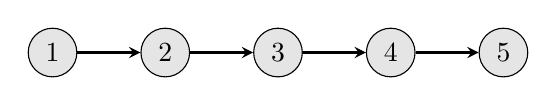
\begin{tikzpicture}
[my/.style={draw, circle, fill=gray!20!}]
\node[my] (1) at(0,0) {1};
\node[my] (2) [right=8mm of 1] {2};
\node[my] (3) [right=8mm of 2] {3};
\node[my] (4) [right=8mm of 3] {4};
\node[my] (5) [right=8mm of 4] {5};
\draw[thick, >=stealth, ->] (1) --(2);
\draw[thick, >=stealth, ->] (2) --(3);
\draw[thick, >=stealth, ->] (3) --(4);
\draw[thick, >=stealth, ->] (4) --(5);
\end{tikzpicture}
\end{figure}
and $ n=2 $
\\
\textbf{Output:}
\begin{figure}[H]
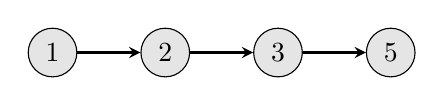
\begin{tikzpicture}
[my/.style={draw, circle, fill=gray!20!}]
\node[my] (1) at(0,0) {1};
\node[my] (2) [right=8mm of 1] {2};
\node[my] (3) [right=8mm of 2] {3};
\node[my] (4) [right=8mm of 3] {5};
\draw[thick, >=stealth, ->] (1) --(2);
\draw[thick, >=stealth, ->] (2) --(3);
\draw[thick, >=stealth, ->] (3) --(4);
\end{tikzpicture}
\end{figure}
\end{flushleft}

\paragraph{Note:}

\begin{itemize}
\item Given $ n $ will always be valid.
\end{itemize}

\paragraph{Follow up:}

\begin{itemize}
\item Could you do this in one pass?
\end{itemize}

\subsection{Two Pointers}
\begin{itemize}
\item 使用两个指针$ x $和$ y $。
\item 创建一个dummy node $ z $,指向head node。
\item 最开始,$ x $初始化为dummy node,而$ y $则是head node。
\item 当$ y $走到第$n+1$个node时(假设head是第一个node),$ x $开始移动。
\item 当$ y $走到链表的最后的\texttt{null} node时,$ x $的下一个node就是需要移除的node。
\item 最后返回dummy的下一个node。使用dummy的原因是,有可能要移除head node。
\end{itemize}

\setcounter{lstlisting}{0}
\begin{lstlisting}[style=customc, caption={Two Pointers}]
ListNode* removeNthFromEnd( ListNode* head, int n )
{
    auto z = new ListNode( -1 );
    z->next = head;

    auto y = head;
    auto x = z;

    int count = 0;

    while( y )
    {
        y = y->next;
        ++count;

        if( count > n )
        {
            //only when y is after (n+1)th
            //x then move
            x = x->next;
        }
    }

    //Just remove the next node of x
    auto next = x->next;
    x->next = next->next;
    x->next = nullptr;

    //The next node of dummy head
    //is the head of new list
    return z->next;

}

\end{lstlisting}

%\section{20 --- Valid Parentheses}
Given a string containing just the characters `(', `)', `\{', `\}', `[' and `]', determine if the input string is valid.
\par
An input string is valid if:
\begin{itemize}
\item Open brackets must be closed by the same type of brackets.
\item Open brackets must be closed in the correct order.
\end{itemize}
\subsection{Stack}
\begin{itemize}
\item Create a stack.
\item if current character is open symbol, push into the stack.
\item Otherwise, check if the top of the stack is the corresponding open symbol. If it is not, return \texttt{false} immediately. Otherwise, pop the top from the stack.
\item Finally, check if the stack is empty.
\end{itemize}
\setcounter{lstlisting}{0}
\begin{lstlisting}[style=customc, caption={Stack}]
bool isValid( string s )
{
    if( s.empty() )
    {
        return true;
    }

    stack<char> stk;

    for( auto c : s )
    {
        switch( c )
        {
        case '{':
        case '(':
        case '[':
            stk.push( c );
            break;

        //need to check if the stack is empty or not
        case '}':
            if( stk.empty() || stk.top() != '{' )
            {
                return false;
            }
            stk.pop();
            break;

        case ')':
            if( stk.empty() || stk.top() != '(' )
            {
                return false;
            }
            stk.pop();
            break;

        case ']':
            if( stk.empty() || stk.top() != '[' )
            {
                return false;
            }
            stk.pop();
            break;
        }
    }

    return stk.empty();
}
\end{lstlisting}

%\section{21 --- Merge Two Sorted Lists}
Merge two sorted linked lists $A$ and $B$ and return it as a new list. The new list should be made by splicing together the nodes of the first two lists.

\paragraph{Example:}

\begin{flushleft}
\textbf{Input}: 
\begin{figure}[H]
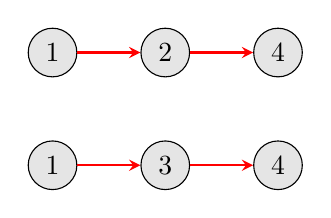
\begin{tikzpicture}
[my/.style={draw, circle, fill=gray!20!, minimum size=5mm}]
\node[my] (0) at (0,0) {1};
\node[my] (1) [right=8mm of 0] {2};
\node[my] (2) [right=8mm of 1] {4};
\draw[thick,>=stealth,->,red] (0) -- (1); 
\draw[thick,>=stealth,->,red] (1) -- (2);

\node[my] (3) [below=8mm of 0] {1};
\node[my] (4) [right=8mm of 3] {3};
\node[my] (5) [right=8mm of 4] {4};
\draw[thick,>=stealth,->,red] (3) -- (4); 
\draw[thick,>=stealth,->,red] (4) -- (5);
\end{tikzpicture}
\end{figure}

\textbf{Output}:
\begin{figure}[H]
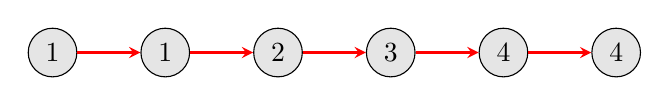
\begin{tikzpicture}
[my/.style={draw, circle, fill=gray!20!, minimum size=5mm}]
\node[my] (0) at (0,0) {1};
\node[my] (1) [right=8mm of 0] {1};
\node[my] (2) [right=8mm of 1] {2};
\node[my] (3) [right=8mm of 2] {3};
\node[my] (4) [right=8mm of 3] {4};
\node[my] (5) [right=8mm of 4] {4};
\draw[thick,>=stealth,->,red] (0) -- (1); 
\draw[thick,>=stealth,->,red] (1) -- (2);
\draw[thick,>=stealth,->,red] (2) -- (3);
\draw[thick,>=stealth,->,red] (3) -- (4);
\draw[thick,>=stealth,->,red] (4) -- (5);
\end{tikzpicture}
\end{figure}
%1->2->4, 1->3->4
%Output: 1->1->2->3->4->4
\end{flushleft}

\subsection{Merge Sort}
\begin{itemize}
\item Create a dummy header
\item From this dummy node, add nodes with smaller values from $A$ or $B$
\item Finally, return the next node of the dummy header.
\end{itemize}

\setcounter{lstlisting}{0}
\begin{lstlisting}[style=customc, caption={Merge Sort}]
ListNode* mergeTwoLists( ListNode* l1, ListNode* l2 )
{
    if( !l1 )
    {
        return l2;
    }

    if( !l2 )
    {
        return l1;
    }

    auto dummy = new ListNode( -1 );


    auto node = dummy;
    auto n1 = l1;
    auto n2 = l2;

    while( n1 && n2 )
    {
        if( n1->val <= n2->val )
        {
            node->next = n1;
            n1 = n1->next;
        }
        else
        {
            node->next = n2;
            n2 = n2->next;
        }

        node = node->next;
    }

    //just link the non null list
    //no need to iterate
    if( n1 )
    {
        node->next = n1;
    }

    if( n2 )
    {
        node->next = n2;
    }


    return dummy->next;
}
\end{lstlisting}

\subsection{Recursion}
\begin{itemize}
\item if current node of $A$'s value is less than or equal to current node of $B$, set current node's next pointer to 
\end{itemize}
%\section{22 --- Generate Parentheses}
Given $ n $ pairs of parentheses, write a function to generate all combinations of well-formed parentheses.
\par
For example, given $ n = 3 $, a solution set is:
\begin{table}[H]
\begin{tabular}{c}
$ ((())) $\\
  $ (()()) $\\
$   (())() $\\
$   ()(()) $\\
$   ()()() $
\end{tabular}
\end{table}

\subsection{Backtracking}
\begin{itemize}
\item To generate all sequences, use a recursion. 
\item All sequences of length $n$ is just a open parenthesis plus all sequences of length $n-1$, and then a close parenthesis plus all sequences of length $n-1$.
\item However, only add them when it will remain a valid sequence by keeping track of the number of opening and closing brackets that have been placed so far.
\end{itemize}


\setcounter{algorithm}{0}
\begin{algorithm}[H]
\caption{Backtracking}
\begin{algorithmic}[1]
\Procedure{GenerateParenthesis}{$N$}
\State $ \star $ Initialize an empty array $A$ to save the results
\State $\ast$ Call recursive helper function \texttt{DFS}
\State \Call{DFS}($A=A, S=\varnothing, x=0, y=0, n$) \Comment Start with empty string, 0 openings and 0 closings
\EndProcedure
\end{algorithmic}
\end{algorithm}

Helper function \texttt{DFS} generate all valid parenthesis strings by tracking $x$ opening and $y$ closings.

\begin{algorithm}[H]
\caption{Recursive Helper Function}
\begin{algorithmic}[1]
\Function{DFS}{$A, S, x, y, n$}
\If{$x+y =2\times n$} \Comment Number of opening and closing parenthesis both are equal to $n$
\State $\star$ Add current string $S$ into $A$
\State \Return
\EndIf
\algstore{22algo}
\end{algorithmic}
\end{algorithm}
\begin{algorithm}[H]
\begin{algorithmic}[1]
\algrestore{22algo}
\If{$x < n$}
\State $\star$ Add an opening parenthesis to $S$
\State $\ast$ Recursively generate with remaining part
\State \Call{DFS}{$ A, S, x+1, y, n $} \Comment Increments number of opening parenthesis 
\EndIf

\If{$y < x$} \Comment We only add closing parenthesis when its number is less than openings
\State $\star$ Add a closing parenthesis to $S$
\State $\ast$ Recursively generate with remaining part
\State \Call{DFS}{$ A, S, x, y+1, n $} \Comment Increments number of closing parenthesis 
\EndIf
\EndFunction
\end{algorithmic}
\end{algorithm}

\setcounter{lstlisting}{0}
\begin{lstlisting}[style=customc, caption={Backtracking}]
vector<string> generateParenthesis( int n )
{
    vector<string> ans;
    string s;

    dfs( ans, s, 0, 0, n );

    return ans;
}

void dfs( vector<string>& A, string S, int x, int y, int n )
{
    if( x + y == n * 2 )
    {
        A.emplace_back( S );
        return;
    }

    if( x < n )
    {
        S.push_back( '(' );
        dfs( A, S, x + 1, y, n );
        S.pop_back();
    }

    if( y < x )
    {
        //only add closing parenthesis when
        //current number of closings are
        //less than current number of openings
        S.push_back( ')' );
        dfs( A, S, x, y + 1, n );
        S.pop_back();
    }
}

\end{lstlisting}

%\section{23 --- Merge k Sorted Lists}
Merge $ k $ sorted linked lists and return it as one sorted list. Analyze and describe its complexity.

\paragraph{Example:}

\begin{flushleft}
\textbf{Input:}
\begin{figure}[H]
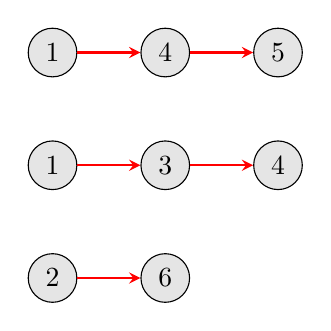
\begin{tikzpicture}
[my/.style={draw, circle, fill=gray!20!, minimum size=5mm}]
\node[my] (0) at (0,0) {1};
\node[my] (1) [right=8mm of 0] {4};
\node[my] (2) [right=8mm of 1] {5};
\draw[thick,>=stealth,->,red] (0) -- (1); 
\draw[thick,>=stealth,->,red] (1) -- (2);

\node[my] (3) [below=8mm of 0] {1};
\node[my] (4) [right=8mm of 3] {3};
\node[my] (5) [right=8mm of 4] {4};
\draw[thick,>=stealth,->,red] (3) -- (4); 
\draw[thick,>=stealth,->,red] (4) -- (5);

\node[my] (6) [below=8mm of 3] {2};
\node[my] (7) [right=8mm of 6] {6};
\draw[thick,>=stealth,->,red] (6) -- (7); 

\end{tikzpicture}
\end{figure}

\textbf{Output:} 
\begin{figure}[H]
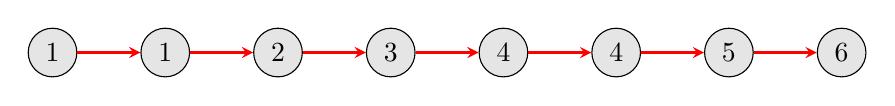
\begin{tikzpicture}
[my/.style={draw, circle, fill=gray!20!, minimum size=5mm}]
\node[my] (0) at (0,0) {1};
\node[my] (1) [right=8mm of 0] {1};
\node[my] (2) [right=8mm of 1] {2};
\node[my] (3) [right=8mm of 2] {3};
\node[my] (4) [right=8mm of 3] {4};
\node[my] (5) [right=8mm of 4] {4};
\node[my] (6) [right=8mm of 5] {5};
\node[my] (7) [right=8mm of 6] {6};
\draw[thick,>=stealth,->,red] (0) -- (1); 
\draw[thick,>=stealth,->,red] (1) -- (2);
\draw[thick,>=stealth,->,red] (2) -- (3);
\draw[thick,>=stealth,->,red] (3) -- (4);
\draw[thick,>=stealth,->,red] (4) -- (5);
\draw[thick,>=stealth,->,red] (5) -- (6);
\draw[thick,>=stealth,->,red] (6) -- (7);
\end{tikzpicture}
\end{figure}

\end{flushleft}
%\section{24 --- Swap Nodes in Pairs}
Given a linked list $L$, swap every two adjacent nodes and return its head.

You may not modify the values in the list's nodes, only nodes itself may be changed.


\paragraph{Example:}
\begin{flushleft}
\textbf{Input}:
\begin{figure}[H]
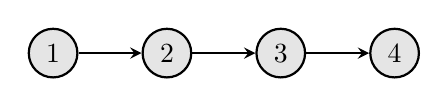
\begin{tikzpicture}
[start chain, every node/.style={draw, circle, minimum size=6mm, fill=gray!20!}, thick, node distance = 8mm, every join/.style={>=stealth,->}]
\node[on chain,] {1};
\node[on chain, join] {2};
\node[on chain, join] {3};
\node[on chain, join] {4};
\end{tikzpicture}
\end{figure}

\textbf{Output}:
\begin{figure}[H]
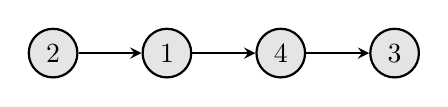
\begin{tikzpicture}
[start chain, every node/.style={draw, circle, minimum size=6mm, fill=gray!20!}, thick, node distance = 8mm, every join/.style={>=stealth,->}]
\node[on chain,] {2};
\node[on chain, join] {1};
\node[on chain, join] {4};
\node[on chain, join] {3};
\end{tikzpicture}
\end{figure}

\end{flushleft}
%\section{25 --- Reverse Nodes in k-Group}
Given a linked list, reverse the nodes of a linked list $k$ at a time and return its modified list.

$k$ is a positive integer and is less than or equal to the length of the linked list. If the number of nodes is not a multiple of k then left-out nodes in the end should remain as it is.

\paragraph{Example:}

\begin{flushleft}
Given this linked list: 

\begin{figure}[H]
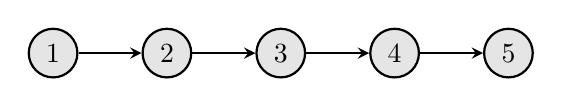
\begin{tikzpicture}
[start chain, every node/.style={draw, circle, minimum size=6mm, fill=gray!20!}, node distance=8mm, every join/.style={>=stealth,->}, thick]
\node[on chain] {1};
\node[on chain, join] {2};
\node[on chain, join] {3};
\node[on chain, join] {4};
\node[on chain, join] {5};
\end{tikzpicture}
\end{figure}
For k = 2, you should return:

\begin{figure}[H]
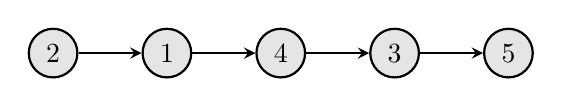
\begin{tikzpicture}
[start chain, every node/.style={draw, circle, minimum size=6mm, fill=gray!20!}, node distance=8mm, every join/.style={>=stealth,->}, thick]
\node[on chain] {2};
\node[on chain, join] {1};
\node[on chain, join] {4};
\node[on chain, join] {3};
\node[on chain, join] {5};
\end{tikzpicture}
\end{figure}

For k = 3, you should return: 
\begin{figure}[H]
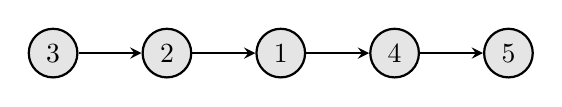
\begin{tikzpicture}
[start chain, every node/.style={draw, circle, minimum size=6mm, fill=gray!20!}, node distance=8mm, every join/.style={>=stealth,->}, thick]
\node[on chain] {3};
\node[on chain, join] {2};
\node[on chain, join] {1};
\node[on chain, join] {4};
\node[on chain, join] {5};
\end{tikzpicture}
\end{figure}

\end{flushleft}


\paragraph{Note:}

\begin{itemize}
\item Only constant extra memory is allowed.
\item You may not alter the values in the list's nodes, only nodes itself may be changed.
\end{itemize}

\subsection{Pointer Operation}
以图中给出的链表为例, 创建一个\texttt{dummy node},因为翻转链表时头结点可能会变化,那么加入这个node后的链表变为
\begin{figure}[H]
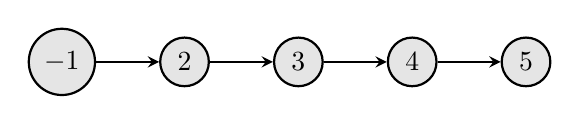
\begin{tikzpicture}
[start chain, 
every node/.style={draw, circle,
 minimum size=6mm, fill=gray!20!},
  node distance=8mm, 
  every join/.style={>=stealth,->},
 thick
]
\node[on chain] {$-1$};
\node[on chain, join] {2};
\node[on chain, join] {3};
\node[on chain, join] {4};
\node[on chain, join] {5};
\end{tikzpicture}
\end{figure}

如果$k$为3的话,目标是将1, 2, 3翻转一下,需要维护两个 pointers: $x$和$y$,分别指向需要翻转的$k$个nodes部分的前后位置,如下图所示

\begin{figure}[H]
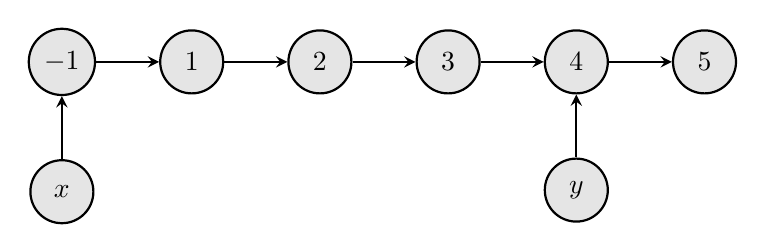
\begin{tikzpicture}
[start chain, 
every node/.style={draw, circle,
 minimum size=8mm, fill=gray!20!},
  node distance=8mm and 8mm, 
  every join/.style={>=stealth,->},
 thick
]
\node(1)[on chain] {$-1$};
\node(x)[below=of 1] {$x$};
\node[on chain, join] {1};
\node[on chain, join] {2};
\node[on chain, join] {3};
\node(4)[on chain, join] {4};
\node(y) [below=of 4] {$y$};
\node[on chain, join] {5};
\draw[>=stealth,->] (x) -- (1);
\draw[>=stealth,->] (y) -- (4);
\end{tikzpicture}
\end{figure}

reverse完成后,$x$更新到下图所示的位置:

\begin{figure}[H]
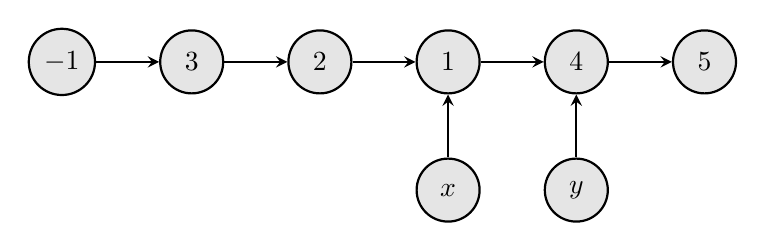
\begin{tikzpicture}
[start chain, 
every node/.style={draw, circle,
 minimum size=8mm, fill=gray!20!},
  node distance=8mm and 8mm, 
  every join/.style={>=stealth,->},
 thick
]
\node(1)[on chain] {$-1$};
\node[on chain, join] {3};
\node(2)[on chain, join] {2};
\node(3)[on chain, join] {1};
\node(4)[on chain, join] {4};
\node[on chain, join] {5};
\node(x)[below=of 3] {$x$};
\node(y) [below=of 4] {$y$};
\draw[>=stealth,->] (x) -- (3);
\draw[>=stealth,->] (y) -- (4);
\end{tikzpicture}
\end{figure}

以此类推,只要\texttt{y}走过$k$个节点,就可以进行局部翻转了。反转过程可参见下面的示意图。

给定的链表如下图所示: 其中start node is $S$, end node is $E$. To reverse node between $S$ and $E$

\begin{figure}[H]
\centering
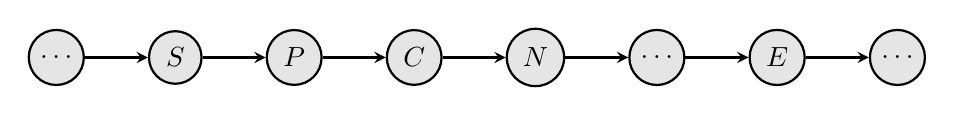
\begin{tikzpicture}
[start chain, 
every node/.style={draw, circle,
 minimum size=6mm, fill=gray!20!},
  node distance=8mm, 
  every join/.style={>=stealth,->},
 thick
]
\node[on chain] {$\ldots$};
\node[on chain, join](1) {$S$};
\node[on chain, join](2) {$P$};
\node[on chain, join](3) {$C$};
\node[on chain, join](4) {$N$};
\node[on chain, join] {$\ldots$};
\node[on chain, join](5) {$E$};
\node[on chain, join] {$\ldots$};
\end{tikzpicture}
\end{figure}

\begin{figure}[H]
\label{fig01}
\caption{Break $P$ with $C$ and link $P$ to $N$}
\centering
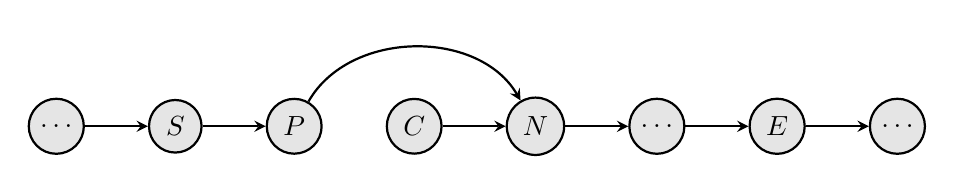
\begin{tikzpicture}
[start chain, 
every node/.style={draw, circle,
 minimum size=6mm, fill=gray!20!},
  node distance=8mm, 
  every join/.style={>=stealth,->},
 thick
]
\node[on chain] {$\ldots$};
\node[on chain, join](1) {$S$};
\node[on chain, join](2) {$P$};
\node[on chain](3) {$C$};
\node[on chain, join](4) {$N$};
\node[on chain, join] {$\ldots$};
\node[on chain, join](5) {$E$};
\node[on chain, join] {$\ldots$};
\draw[>=stealth, ->] (2) [bend left=60] to (4);
\end{tikzpicture}
\end{figure}

\begin{figure}[H]
\caption{Break $C$ with $N$ and set $C$ to next node of $S$}
\centering
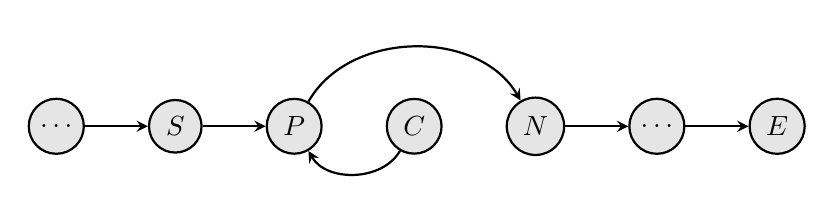
\begin{tikzpicture}
[start chain, 
every node/.style={draw, circle,
 minimum size=6mm, fill=gray!20!},
  node distance=8mm, 
  every join/.style={>=stealth,->},
 thick
]
\node[on chain] {$\ldots$};
\node[on chain, join](1) {$S$};
\node[on chain, join](2) {$P$};
\node[on chain](3) {$C$};
\node[on chain](4) {$N$};
\node[on chain, join] {$\ldots$};
\node[on chain, join](5) {$E$};
\draw[>=stealth, ->] (2) [bend left=60] to (4);
\draw[>=stealth, ->] (3) [bend left=60] to (2);
\end{tikzpicture}
\end{figure}

\begin{figure}[H]
\caption{Break $S$ and $P$, link $S$ to $C$}
\centering
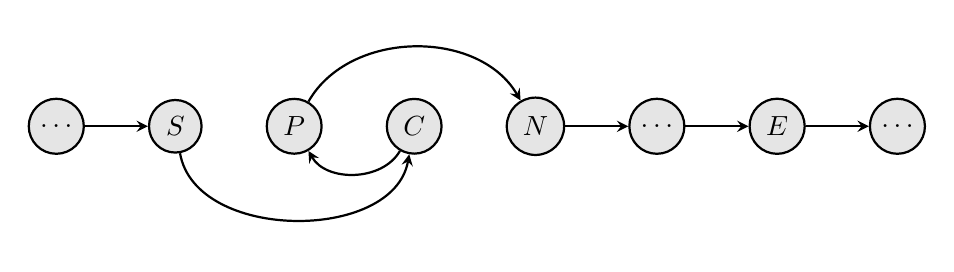
\begin{tikzpicture}
[start chain, 
every node/.style={draw, circle,
 minimum size=6mm, fill=gray!20!},
  node distance=8mm, 
  every join/.style={>=stealth,->},
 thick
]
\node[on chain] {$\ldots$};
\node[on chain, join](1) {$S$};
\node[on chain](2) {$P$};
\node[on chain](3) {$C$};
\node[on chain](4) {$N$};
\node[on chain, join] {$\ldots$};
\node[on chain, join](5) {$E$};
\node[on chain, join] {$\ldots$};
\draw[>=stealth, ->] (2) [bend left=60] to (4);
\draw[>=stealth, ->] (3) [bend left=60] to (2);
\draw[>=stealth, ->] (1) [bend left=280] to (3);
\end{tikzpicture}
\end{figure}


\begin{figure}[H]
\caption{Set next node of $S$ to $C$}
\centering
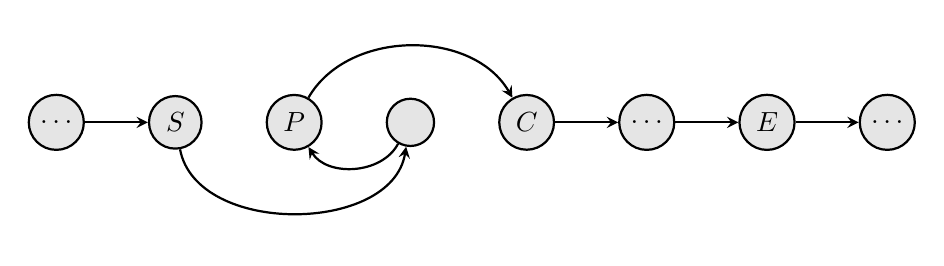
\begin{tikzpicture}
[start chain, 
every node/.style={draw, circle,
 minimum size=6mm, fill=gray!20!},
  node distance=8mm, 
  every join/.style={>=stealth,->},
 thick
]
\node[on chain] {$\ldots$};
\node[on chain, join](1) {$S$};
\node[on chain](2) {$P$};
\node[on chain](3) {};
\node[on chain](4) {$C$};
\node[on chain, join] {$\ldots$};
\node[on chain, join](5) {$E$};
\node[on chain, join] {$\ldots$};
\draw[>=stealth, ->] (2) [bend left=60] to (4);
\draw[>=stealth, ->] (3) [bend left=60] to (2);
\draw[>=stealth, ->] (1) [bend left=280] to (3);
\end{tikzpicture}
\end{figure}

By the figures shows above, we put previous $C$ before $P$ and link $S$ to $C$. Then move $C$ to previous $N$, and repeat the process by staring similarly to figure \ref{fig01}.

At the end of the reverse, $C$ will be at $E$, while $P$ is not moved and the next node of $S$ is the previous node of $E$.

\begin{figure}[H]
\caption{Update $C$ to $P$'s next node}
\centering
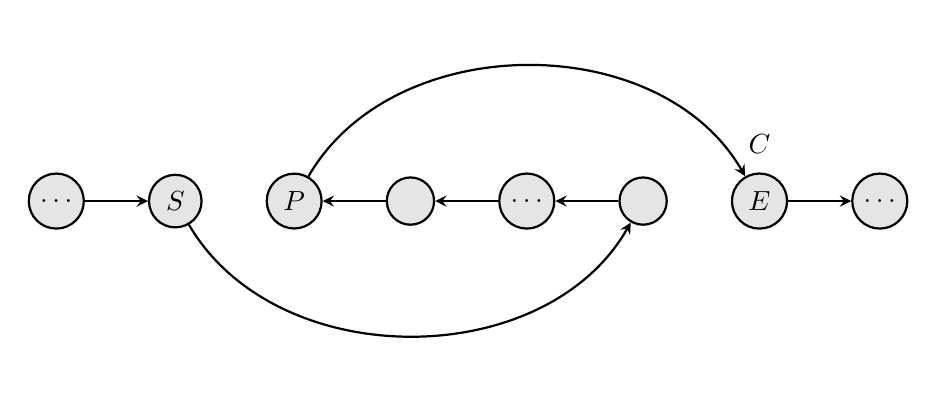
\begin{tikzpicture}
[start chain, 
every node/.style={draw, circle,
 minimum size=6mm, fill=gray!20!},
  node distance=8mm, 
  every join/.style={>=stealth,->},
 thick
]
\node[on chain] {$\ldots$};
\node[on chain, join](1) {$S$};
\node[on chain](2) {$P$};
\node[on chain](3) {};
\node[on chain](4) {$\ldots$};
\node[on chain](T) {};
\node[on chain, label=above:$C$](5) {$E$};
\node[on chain, join] {$\ldots$};
\draw[>=stealth,->] (2) [bend left=60] to (5);
\draw[>=stealth,->] (1) [bend left=300] to (T);
\draw[>=stealth,->] (T) -- (4);
\draw[>=stealth,->] (4) -- (3);
\draw[>=stealth,->] (3) -- (2);
\end{tikzpicture}
\end{figure}


\setcounter{algorithm}{0}
\begin{algorithm}[H]
\caption{Reverse link list by $k$ steps}
\begin{algorithmic}[1]
\Procedure{ReverseKGroup}{$L, K$}
\State $\star$ Create a dummy node $d$.
\State $s:=d$ \Comment The pointer to the previous node of the group to be reversed
\State $\star$ Link $s$ to $L$ \Comment Link dummy node to the linked list
\State $\ast$ Start the process
\State $c:=L$ \Comment Current Node
\State $\delta:=0$ \Comment The counter
\While{$c$ is not null}
\State $\delta\gets\delta + 1$
\If{$\delta=K$}
\State $\delta=0$
\State $s\gets$\Call{Reverse}{$s, c_n$} \Comment Reverse the group starting with next node of $s$ and ending with $c$
\State $\star$ Update $c$ as the next node of $x$
\Else
\State $\star$ Update $c$ to its next node
\EndIf
\EndWhile
\EndProcedure
\end{algorithmic}
\end{algorithm}

Function \texttt{Reverse} reverse the segment in list between start node $s$ and end node $e$

\begin{algorithm}[H]
\caption{Reverse one segment of link list }
\begin{algorithmic}[1]
\Function{Reverse}{$s,e$}
\State $p := s_n$ \Comment $x$ is the next node of $s$
\State $\ast$ Starting reverse from next node of $x$
\State $c := p_n$ 
\While{$c \neq e$}
\State $\ast$ Break $p$ with $c$, and link $p$ to next node of $c$
\State $p_n \gets c_n $
\State $\ast$ Set next node of $c$ to next node of $s$
\State $c_n \gets s_n $ 
\State $\ast$ Set next node of $s$ to $c$
\State $s_n \gets c$ 
\State $\ast$ Update $c$ as next node of $p$
\State $c\gets p_n$
\EndWhile
\State \Return $p$ \Comment next node of $p$ is the start of next group
\EndFunction
\end{algorithmic}
\end{algorithm}


\setcounter{lstlisting}{0}
\begin{lstlisting}[style=customc, caption={Pointer operation}]
ListNode* reverseKGroup( ListNode* head, int k )
{
    ListNode* dummy = new ListNode( 0 );

    auto S = dummy;

    //link S to head
    S->next = head;

    auto x = head;

    int count = 0;

    while( x != nullptr )
    {
        //since count starting with zero
        //increment count first
        ++count;

        if( count == k )
        {
            count = 0;
            //reverse S to x->next
            S = reverse( S, x->next );
            //update x to S->next
            x = S->next;
        }
        else
        {
            x = x->next;
        }
    }

    return dummy->next;
}
//Helper function to reverse between S and E
ListNode* reverse( ListNode* S, ListNode* E )
{
    auto P = S->next;

    auto C = P->next;

    while( C != E )
    {
        //break P with C and link to C->next
        P->next = C->next;

        //link C to S->next
        C->next = S->next;

        //link S to C
        S->next = C;

        //update C to P->next
        C = P->next;
    }

    //P->next is the start of next group
    return P;
}
\end{lstlisting}
%\section{26 --- Remove Duplicates from Sorted Array}

Given a sorted array $A$, remove the duplicates in-place such that each element appear only once and return the new length.

Do not allocate extra space for another array, you must do this by modifying the input array in-place with $O(1)$ extra memory.

\paragraph{Example 1:}

\begin{flushleft}
\textbf{Input}: $A = [1,1,2]$

\textbf{Output}: 2

\textbf{Explanation}: Your function should return length equal to 2 with the first two elements of $A$ being 1 and 2 respectively.
\end{flushleft}

\paragraph{Example 2:}

\begin{flushleft}
\textbf{Input}: $A = [0,0,1,1,1,2,2,3,3,4]$

\textbf{Output}: 5

\textbf{Explanation}: 
Your function should return length equal to 5, with the first five elements of nums being modified to 0, 1, 2, 3, and 4 respectively. 

It doesn't matter what values are set beyond the returned length.
\end{flushleft}

\subsection{Binary Search With Two Pointers}
\begin{itemize}
\item 用一个write指针代表写入的位置,用read指针从$A$中读取数字。
\item 遇到重复数字,用rightmost binary search快速定位第一个与当前数字不同的数字。
\end{itemize}

\setcounter{lstlisting}{0}
\begin{lstlisting}[style=customc, caption={Binary Search With Two Pointers}]
int removeDuplicates( vector<int>& nums )
{
    int L = static_cast<int>( nums.size() );

    int write = 0;

    int i = 0;

    while( i < L )
    {
        if( i == L - 1 )
        {
            nums[write] = nums[i];
            ++write;
            break;
        }

        if( nums[i] == nums[i + 1] )
        {
            //search for the end of duplicate
            //by binary search

            int l = i;
            int r = L;

            //rightmost binary search
            //find the first element
            //that is larger than nums[i]

            while( l < r )
            {
                int m = ( l + r ) / 2;
                if( nums[m] <= nums[i] )
                {
                    l = m + 1;
                }
                else
                {
                    r = m;
                }
            }

            //write current element into write
            nums[write] = nums[i];
            //increments the write
            ++write;

            //set next start at l
            i = l;
        }
        else
        {
            //nums[i] is not duplicate
            //directly put into write
            nums[write] = nums[i];
            //increments the write
            ++write;
            //increments i
            ++i;
        }
    }

    //nums[0...write-1] are all unique elements
    return write;
}
\end{lstlisting}



%\section{27 --- Remove Element}
Given an array $A$ and a value $x$, remove all instances of that value in-place and return the new length.

Do not allocate extra space for another array, you must do this by modifying the input array in-place with $O(1)$ extra memory.

The order of elements can be changed. It doesn't matter what you leave beyond the new length.

\paragraph{Example 1:}
\begin{flushleft}
\textbf{Input}: $A=[3,2,2,3]$, $x=3$

\textbf{Output}: 2

\textbf{Explanation}: 

Your function should return 2 with the first two elements of $A$ being 2. 

It doesn't matter what you leave beyond the returned length.
\end{flushleft}

\paragraph{Example 2:}

\begin{flushleft}
\textbf{Input}: $A = [0,1,2,2,3,0,4,2]$, $x = 2$,

\textbf{Output}: 5

\end{flushleft}

\subsection{Double Pointers}
\begin{itemize}
\item 同样是双指针,遇到与$x$不相等的,写入write指针的位置,然后increments write指针。
\end{itemize}

\setcounter{lstlisting}{0}
\begin{lstlisting}[style=customc, caption={Double Pointers}]
int removeElement( vector<int>& nums, int val )
{
    size_t write = 0;

    size_t read = 0;

    while( read < nums.size() )
    {
        if( nums[read] != val )
        {
            //put to write position
            nums[write] = nums[read];
            ++write;
        }

        ++read;
    }

    return write;
}
\end{lstlisting}
%\section{28 --- Implement strStr()}
Implement function \texttt{strStr}().

Return the index of the first occurrence of \textbf{needle} in \textbf{haystack}, or $-1$ if \textbf{needle} is not part of \textbf{haystack}.

\paragraph{Example 1:}

\begin{flushleft}
\textbf{Input}: \textbf{haystack} = \texttt{hello}, \textbf{needle} = \texttt{ll}


\textbf{Output}: 2
\end{flushleft}

\paragraph{Example 2:}

\begin{flushleft}
\textbf{Input}: \textbf{haystack} = \texttt{aaaaa}, \textbf{needle} = \texttt{bba}

\textbf{Output}: $-1$
\end{flushleft}

\paragraph{Clarification}:

\begin{flushleft}
What should we return when needle is an empty string? This is a great question to ask during an interview.

For the purpose of this problem, we will return 0 when needle is an empty string. 
\end{flushleft}

\subsection{KMP}
\begin{itemize}
\item 网上很多KMP算法介绍中,table包含$-1$。
\item 这里的KMP算法中的table不包含$-1$,因此当找到两个不匹配的字符时,如果pattern的当前位置$y$不为零,则$y\gets f(y-1)$,其中$f$为得到的pattern字符串的table。而如果$y$为零,则increments被搜寻字符串中的index $x$。
\end{itemize}

\setcounter{lstlisting}{0}
\begin{lstlisting}[style=customc, caption={KMP}]
int strStr( string haystack, string needle )
{
    if( needle.empty() )
    {
        return 0;
    }

    if( haystack.empty() )
    {
        return -1;
    }

    vector<int> f( needle.size(), 0 );

    int t = 0;

    //generate pattern table for needle
    for( size_t i = 1; i < needle.size(); ++i )
    {
        t = f[i - 1];

        while( ( t > 0 ) && ( needle[i] != needle[t] ) )
        {
            t = f[t - 1];
        }

        if( needle[i] == needle[t] )
        {
            t = t + 1;
        }

        f[i] = t;
    }

    //index in haystack
    size_t x = 0;
    //index in needle
    size_t y = 0;

    while( x < haystack.size() )
    {
        if( haystack[x] == needle[y] )
        {
            ++x;
            ++y;

            if( y == needle.size() )
            {
                //returns the start index
                //of the matching
                return x - y;
            }
        }
        else
        {
            if( y > 0 )
            {
                //get the next search index
                //in the pattern from f[y-1]
                y = f[y - 1];
            }
            else
            {
                //otherwise
                //increments the index in
                //haystack
                ++x;
            }
        }

    }

    return -1;

}
\end{lstlisting}
%\section{29 --- Divide Two Integers}
Given two integers $A$ and $B$, divide $A$ by $B$ without using multiplication, division and mod operator.

Return the quotient after dividing dividend by divisor.

The integer division should truncate toward zero.

\paragraph{Example 1:}

\begin{flushleft}
\textbf{Input}: $A = 10$, $B = 3$

\textbf{Output}: 3
\end{flushleft}

\paragraph{Example 2:}

\begin{flushleft}
\textbf{Input}: $A = 7$, $B = -3$

\textbf{Output}: $-2$
\end{flushleft}

\paragraph{Note:}

\begin{itemize}
\item Both dividend $A$ and divisor $B$ will be 32-bit signed integers.
\item The divisor $B$ will never be 0.
\item Assume we are dealing with an environment which could only store integers within the 32-bit signed integer range: $[−2^{31},  2^{31} − 1]$. For the purpose of this problem, assume that your function returns $2^{31} − 1$ when the division result overflows.
\end{itemize}

\subsection{Left Shift}
\begin{itemize}
\item 由于每次左移相当于乘以2,因此每次尽量将divisor左移,看最多能左移多少位仍然小于被除数。
\item 找到这个最大的左移位数 $s$ 后,将被除数减去divisor左移这么多位后的结果,同时累加$2^s$到商中。
\item 如果被除数仍然大于或者等于除数,继续上述过程。
\end{itemize}

\setcounter{lstlisting}{0}
\begin{lstlisting}[style=customc, caption={Left Shift}]
int divide( int dividend, int divisor )
{

    if( ( dividend == INT_MIN ) && ( divisor == -1 ) )
    {
        return INT_MAX;
    }


    int sign = 1;
    if( ( dividend > 0 ) && ( divisor < 0 ) )
    {
        sign = -1;
    }

    if( ( dividend < 0 ) && ( divisor > 0 ) )
    {
        sign = -1;
    }

    //change to long long to avoid overflow
    auto x = static_cast<long long>( dividend );
    auto y = static_cast<long long>( divisor );

    //change both to
    //positive numbers
    x = abs( x );
    y = abs( y );


    long long q = 0;


    //the condition is x>=y
    //not x>y because when x can be divided by y
    //quotient is 1
    while( x >= y )
    {
        auto z = y;
        long long count = 1;
        //find 2^{count} * z <= x
        while( ( z << 1 ) < x )
        {
            z <<= 1;
            count <<= 1;
        }

        //add the number of z
        //2^{count}
        q += count;
        //remove from x
        x -= z;
    }

    return q * sign;
}

\end{lstlisting}

%\section{30 --- Substring with Concatenation of All Words}
You are given a string, $s$, and a list of words, $W$, that are all of the same length. Find all starting indices of substring(s) in $s$ that is a concatenation of each word in words exactly once and without any intervening characters.

\paragraph{Example 1:}

\begin{flushleft}
\textbf{Input}: $s = \texttt{barfoothefoobarman}$, $W = [\texttt{foo},\, \texttt{bar}]$

\textbf{Output}: $[0,\,9]$

\textbf{Explanation}: 

Substrings starting at index 0 and 9 are \texttt{barfoor} and \texttt{foobar} respectively. 

The output order does not matter, returning $[9,\,0]$ is fine too.
\end{flushleft}

\paragraph{Example 2:}

\begin{flushleft}
\textbf{Input}: $s = \texttt{wordgoodgoodgoodbestword}$, $W = [\texttt{word},\,\texttt{good},\,\texttt{best},\,\texttt{word}]$

\textbf{Output}: $[\,]$
\end{flushleft}
%\section{31 --- Next Permutation}
Implement \textbf{next permutation}, which rearranges numbers into the lexicographically next greater permutation of numbers.
\par
If such arrangement is not possible, it must rearrange it as the lowest possible order (ie, sorted in ascending order).
\par
The replacement must be in-place and use only constant extra memory.
\par
Here are some examples. Inputs are in the left-hand column and its corresponding outputs are in the right-hand column.
\begin{table}[H]
\begin{tabular}{lcl}
(1,2,3) & $\Longrightarrow$ & (1,3,2) \\
(3,2,1) & $\Longrightarrow$ & (1,2,3) \\
(1,1,5) & $\Longrightarrow$ & (1,5,1)
\end{tabular}
\end{table}
\subsection{Single Pass}
\begin{enumerate}
    \item 如果给定的sequence已经是降序排列,就不会有next permutation。例如 $[9, 5, 4, 3, 1]$
    \item 从右到左寻找the first pair of two successive numbers $a[i]$ and $a[i-1]$, which satisfy $A[i] > A[i-1]$. 由于从$A[i]$到最后一个数都是降序排列,因此这个部分无需进行rearrange。需要rearrang的是从$A[i-1]$到最后一个数。
    \item 由于next permutation is the one just larger than the current one,因此方法就是用$A[i-1]$的右边所有数中,即从$A[i]$到$A[L-1]$中大于$A[i-1]$的数中最小的那个数替换$A[i-1]$。而由于$A[i]$到$A[L-1]$都是降序排列,因此只需从位置$i$开始寻找最后一个大于$A[i-1]$的数即可,假设这个数是$A[j]$。 
    \item Swap $A[i-1]$ and $A[j]$。 这时候$A[i]$到$A[L-1]$仍然是降序排列。为了得到更小的permutation, 需要将其变为升序排列。因此 Reverse $A[i]$ to $A[L-1]$就能得到next permutation了。
\end{enumerate}
\begin{figure}[H]
\begin{tikzpicture}
[mynode/.style={draw,minimum height=1cm, inner sep=0.5 cm, node distance=0.6cm, fill=gray!20!}]
\node[rectangle split, rectangle split horizontal, rectangle split parts=9] (a)[mynode] {$1$ \nodepart{two} $5$ \nodepart{three} $8$ \nodepart{four} $4$ \nodepart{five} $7$ \nodepart{six} $6$ \nodepart{seven} $5$ \nodepart{eight} $3$ \nodepart{nine} $1$};
\node (b) [below=8mm of a.nine south] {};
\node (c) [above=1cm of a] {从右到左寻找第一个decreasing number};
\draw[red, >=stealth,->, line width=2pt] (b) -- (a.nine south);
\end{tikzpicture}
\end{figure}
\begin{figure}[H]
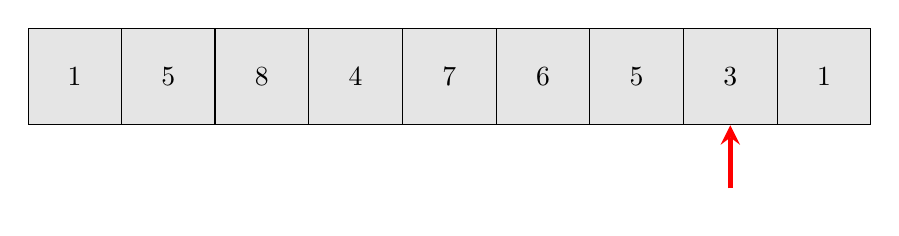
\begin{tikzpicture}
[mynode/.style={draw,minimum height=1cm, inner sep=0.5 cm, node distance=0.6cm, fill=gray!20!}]
\node[rectangle split, rectangle split horizontal, rectangle split parts=9] (a)[mynode] {$1$ \nodepart{two} $5$ \nodepart{three} $8$ \nodepart{four} $4$ \nodepart{five} $7$ \nodepart{six} $6$ \nodepart{seven} $5$ \nodepart{eight} $3$ \nodepart{nine} $1$};
\node (b) [below=8mm of a.eight south] {};
\draw[red, >=stealth,->, line width=2pt] (b) -- (a.eight south);
\end{tikzpicture}
\end{figure}
\begin{figure}[H]
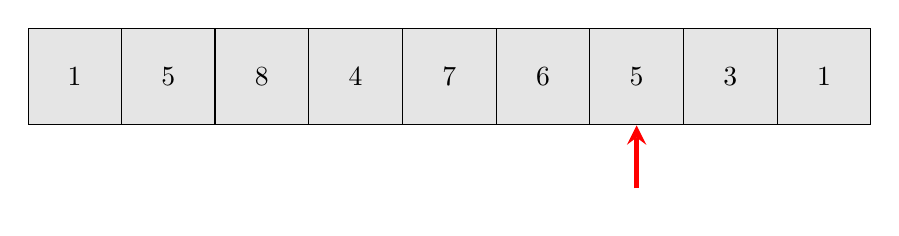
\begin{tikzpicture}
[mynode/.style={draw,minimum height=1cm, inner sep=0.5 cm, node distance=0.6cm, fill=gray!20!}]
\node[rectangle split, rectangle split horizontal, rectangle split parts=9] (a)[mynode] {$1$ \nodepart{two} $5$ \nodepart{three} $8$ \nodepart{four} $4$ \nodepart{five} $7$ \nodepart{six} $6$ \nodepart{seven} $5$ \nodepart{eight} $3$ \nodepart{nine} $1$};
\node (b) [below=8mm of a.seven south] {};
\draw[red, >=stealth,->, line width=2pt] (b) -- (a.seven south);
\end{tikzpicture}
\end{figure}
\begin{figure}[H]
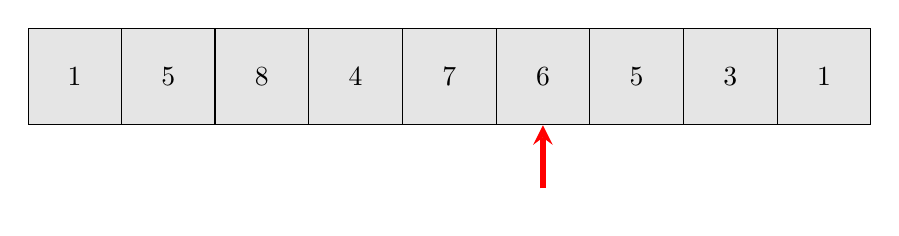
\begin{tikzpicture}
[mynode/.style={draw,minimum height=1cm, inner sep=0.5 cm, node distance=0.6cm, fill=gray!20!}]
\node[rectangle split, rectangle split horizontal, rectangle split parts=9] (a)[mynode] {$1$ \nodepart{two} $5$ \nodepart{three} $8$ \nodepart{four} $4$ \nodepart{five} $7$ \nodepart{six} $6$ \nodepart{seven} $5$ \nodepart{eight} $3$ \nodepart{nine} $1$};
\node (b) [below=8mm of a.six south] {};
\draw[red, >=stealth,->, line width=2pt] (b) -- (a.six south);
\end{tikzpicture}
\end{figure}
\begin{figure}[H]
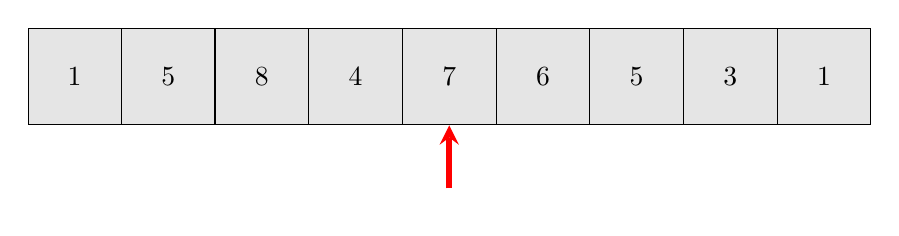
\begin{tikzpicture}
[mynode/.style={draw,minimum height=1cm, inner sep=0.5 cm, node distance=0.6cm, fill=gray!20!}]
\node[rectangle split, rectangle split horizontal, rectangle split parts=9] (a)[mynode] {$1$ \nodepart{two} $5$ \nodepart{three} $8$ \nodepart{four} $4$ \nodepart{five} $7$ \nodepart{six} $6$ \nodepart{seven} $5$ \nodepart{eight} $3$ \nodepart{nine} $1$};
\node (b) [below=8mm of a.five south] {};
\draw[red, >=stealth,->, line width=2pt] (b) -- (a.five south);
\end{tikzpicture}
\end{figure}
\begin{figure}[H]
\begin{tikzpicture}
[mynode/.style={draw,minimum height=1cm, inner sep=0.5 cm, node distance=0.6cm, fill=gray!20!}]
\node[rectangle split, rectangle split horizontal, rectangle split parts=9] (a)[mynode] {$1$ \nodepart{two} $5$ \nodepart{three} $8$ \nodepart{four} $4$ \nodepart{five} $7$ \nodepart{six} $6$ \nodepart{seven} $5$ \nodepart{eight} $3$ \nodepart{nine} $1$};
\node (b) [below=8mm of a.four south] {};
\draw[red, >=stealth,->, line width=2pt] (b) -- (a.four south);
\node (c) [above=1cm of a] {找到了第一个decreasing number = $4$};
\end{tikzpicture}
\end{figure}
\begin{figure}[H]
\begin{tikzpicture}
[mynode/.style={draw,minimum height=1cm, inner sep=0.5 cm, node distance=0.6cm, fill=gray!20!}]
\node[rectangle split, rectangle split horizontal, rectangle split parts=9] (a)[mynode] {$1$ \nodepart{two} $5$ \nodepart{three} $8$ \nodepart{four} $4$ \nodepart{five} $7$ \nodepart{six} $6$ \nodepart{seven} $5$ \nodepart{eight} $3$ \nodepart{nine} $1$};
\node (b) [below=10mm of a.four south] {\textcolor{red}{$A[i-1]$}};
\draw[red, >=stealth,->, line width=2pt] (b) -- (a.four south);
\node (d) [above=1cm of a.five north] {};
\draw[blue, >=stealth,->, line width=2pt] (d) -- (a.five north);
\node (c) [above=2cm of a] {从4开始往右寻找最后一个大于4的number};
\end{tikzpicture}
\end{figure}
\begin{figure}[H]
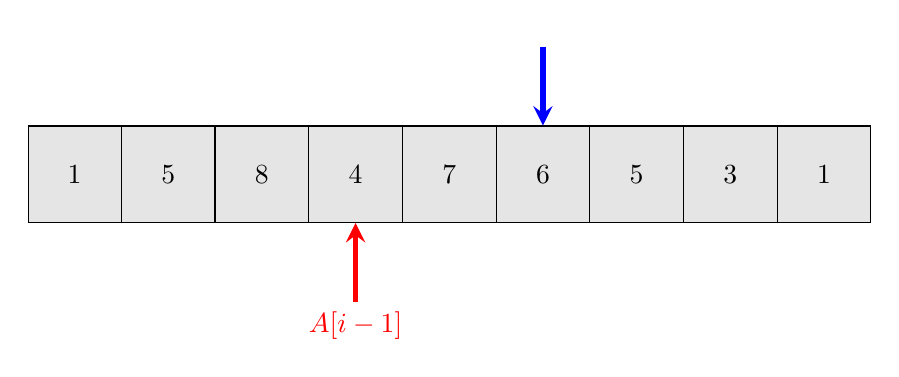
\begin{tikzpicture}
[mynode/.style={draw,minimum height=1cm, inner sep=0.5 cm, node distance=0.6cm, fill=gray!20!}]
\node[rectangle split, rectangle split horizontal, rectangle split parts=9] (a)[mynode] {$1$ \nodepart{two} $5$ \nodepart{three} $8$ \nodepart{four} $4$ \nodepart{five} $7$ \nodepart{six} $6$ \nodepart{seven} $5$ \nodepart{eight} $3$ \nodepart{nine} $1$};
\node (b) [below=10mm of a.four south] {\textcolor{red}{$A[i-1]$}};
\draw[red, >=stealth,->, line width=2pt] (b) -- (a.four south);
\node (d) [above=1cm of a.six north] {};
\draw[blue, >=stealth,->, line width=2pt] (d) -- (a.six north);
\end{tikzpicture}
\end{figure}
\begin{figure}[H]
\begin{tikzpicture}
[mynode/.style={draw,minimum height=1cm, inner sep=0.5 cm, node distance=0.6cm, fill=gray!20!}]
\node[rectangle split, rectangle split horizontal, rectangle split parts=9] (a)[mynode] {$1$ \nodepart{two} $5$ \nodepart{three} $8$ \nodepart{four} $4$ \nodepart{five} $7$ \nodepart{six} $6$ \nodepart{seven} $5$ \nodepart{eight} $3$ \nodepart{nine} $1$};
\node (b) [below=10mm of a.four south] {\textcolor{red}{$A[i-1]$}};
\draw[red, >=stealth,->, line width=2pt] (b) -- (a.four south);
\node (d) [above=1.1cm of a.seven north] {\textcolor{blue}{$A[j]$}};
\draw[blue, >=stealth,->, line width=2pt] (d) -- (a.seven north);
\node (c) [above=2cm of a] {找到了从4往右最后一个大于4的number=5};
\end{tikzpicture}
\end{figure}
%swap
\begin{figure}[H]
\begin{tikzpicture}
[mynode/.style={draw,minimum height=1cm, inner sep=0.5 cm, node distance=0.6cm, fill=gray!20!}]
\node[rectangle split, rectangle split horizontal, rectangle split parts=9] (a)[mynode] {$1$ \nodepart{two} $5$ \nodepart{three} $8$ \nodepart{four} $4$ \nodepart{five} $7$ \nodepart{six} $6$ \nodepart{seven} $5$ \nodepart{eight} $3$ \nodepart{nine} $1$};
\node (b) [below=10mm of a.four south] {\textcolor{red}{$A[i-1]$}};
\draw[red, >=stealth,->, line width=2pt] (b) -- (a.four south);
\node (d) [above=1.1cm of a.seven north] {\textcolor{blue}{$A[j]$}};
\draw[blue, >=stealth,->, line width=2pt] (d) -- (a.seven north);
\node (c) [above=2cm of a] {将4和5的位置进行互换};
\draw [blue,>=stealth,->,line width=2pt,out=105,in=30] (a.seven north) to (a.four north);
\draw [red,>=stealth,->,line width=2pt,out=-15,in=-60] (a.four south) to (a.seven south);
\end{tikzpicture}
\end{figure}
\begin{figure}[H]
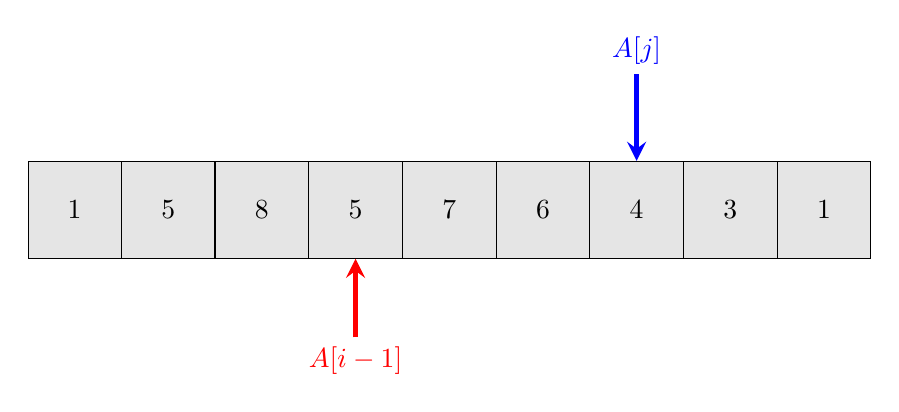
\begin{tikzpicture}
[mynode/.style={draw,minimum height=1cm, inner sep=0.5 cm, node distance=0.6cm, fill=gray!20!}]
\node[rectangle split, rectangle split horizontal, rectangle split parts=9] (a)[mynode] {$1$ \nodepart{two} $5$ \nodepart{three} $8$ \nodepart{four} $5$ \nodepart{five} $7$ \nodepart{six} $6$ \nodepart{seven} $4$ \nodepart{eight} $3$ \nodepart{nine} $1$};
\node (b) [below=10mm of a.four south] {\textcolor{red}{$A[i-1]$}};
\draw[red, >=stealth,->, line width=2pt] (b) -- (a.four south);
\node (d) [above=1.1cm of a.seven north] {\textcolor{blue}{$A[j]$}};
\draw[blue, >=stealth,->, line width=2pt] (d) -- (a.seven north);
\end{tikzpicture}
\end{figure}
%Reverse
\begin{figure}[H]
\begin{tikzpicture}
[mynode/.style={draw,minimum height=1cm, inner sep=0.5 cm, node distance=0.6cm, fill=gray!20!}]
\node[rectangle split, rectangle split horizontal, rectangle split parts=9] (a)[mynode] {$1$ \nodepart{two} $5$ \nodepart{three} $8$ \nodepart{four} $5$ \nodepart{five} $7$ \nodepart{six} $6$ \nodepart{seven} $4$ \nodepart{eight} $3$ \nodepart{nine} $1$};
\node (b) [below=10mm of a.four south] {\textcolor{red}{$A[i-1]$}};
\draw[red, >=stealth,->, line width=2pt] (b) -- (a.four south);
\node (c) [above=1cm of a] {Reverse $A[i-1]$ 后面的数字};
\node (d) [below=1.5cm of a.seven south] {Reverse};
\draw[blue, line width=2pt] (a.four split south) ..  controls +(0,-1.5cm) and +(0,1.5cm) .. (d.north);
\draw[blue, line width=2pt] (a.south east) ..  controls +(0,-1.5cm) and +(0,1.5cm) .. (d.north);
\end{tikzpicture}
\end{figure}
\begin{figure}[H]
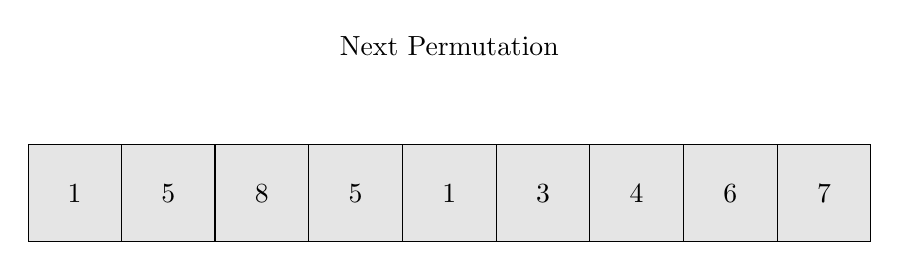
\begin{tikzpicture}
[mynode/.style={draw,minimum height=1cm, inner sep=0.5 cm, node distance=0.6cm, fill=gray!20!}]
\node[rectangle split, rectangle split horizontal, rectangle split parts=9] (a)[mynode] {$1$ \nodepart{two} $5$ \nodepart{three} $8$ \nodepart{four} $5$ \nodepart{five} $1$ \nodepart{six} $3$ \nodepart{seven} $4$ \nodepart{eight} $6$ \nodepart{nine} $7$};
\node (c) [above=1cm of a] {Next Permutation};
\end{tikzpicture}
\end{figure}

\setcounter{algorithm}{0}
\begin{algorithm}[H]
\caption{Find Next Permutation}
\begin{algorithmic}[1]
\Procedure{NextPermutation}{$A, L$}
\State $\star$ 从右到左检查是否存在$A[i]>A[i-1]$
\State $p:=L$ \Comment At $p$, $A[p] > A[p-1]$
\For{$i := L-1$ \textbf{to} $1$}
\If{$A[i] > A[i-1]$}
\State $p\gets i$ \Comment Found the first descending number
\State \textbf{Break}
\EndIf
\EndFor
\If{$p \neq L_A$} \Comment There exits $A[i] > A[i-1]$
\State $\ast$ 寻找$A[p]$到$A[L-1]$中大于$A[p-1]$的所有数中的最小值。
\State $q:=p$ \Comment $A[q] =\min(A[j]\;|\;A[j] > A[p],\ p\leq j<L)$
\For{$j:=p$ \textbf{to} $L-1$}
\If{$A[j] > A[p-1]$}
\State $q\gets j$ \Comment Update $q$ 
\Else
\State \texttt{break}
\EndIf
\EndFor
\algstore{31algo}
\end{algorithmic}
\end{algorithm}
\begin{algorithm}[H]
\begin{algorithmic}[1]
\algrestore{31algo}
\State $\star$ Swap $A[p-1]$ and $A[q]$
\State $\star$ Reverse $A[p]$ to $A[L-1]$
\Else
\State $\ast$ 不存在next permutation 因为$A$已经是降序排列了
\State $\star$ 直接reverse $A$
\EndIf
\EndProcedure
\end{algorithmic}
\end{algorithm}
\setcounter{lstlisting}{0}
\begin{lstlisting}[style=customc, caption={Next Permutation}]
void nextPermutation( vector<int>& nums )
{
    size_t p = nums.size();

    for( size_t i = nums.size() - 1; i >= 1; --i )
    {
        if( nums[i] > nums[i - 1] )
        {
            p = i;
            break;
        }
    }

    if( p != nums.size() )
    {
        //Exists A[i] > A[i-1]
        //Need to find the minimum number thar is larger than A[p-1]

        auto q = p;

        for( size_t j = p; j < nums.size(); ++j )
        {
            if( nums[j] > nums[p - 1] )
            {
                q = j;
            }
            else
            {
                break;
            }
        }

        swap( nums[q], nums[p - 1] );
        reverse( nums.begin() + p, nums.end() );
    }
    else
    {
        //A is decending
        //just reverse A
        reverse( nums.begin(), nums.end() );
    }

}
\end{lstlisting}
%\section{32 --- Longest Valid Parentheses}
Given a string $s$ containing just the characters left and right parenthesis, find the length of the longest valid (well-formed) parentheses substring.

\paragraph{Example 1:}

\begin{flushleft}
\textbf{Input}: \texttt{(()}

\textbf{Output}: 2

\textbf{Explanation}: The longest valid parentheses substring is \texttt{()}
\end{flushleft}

\paragraph{Example 2:}
\begin{flushleft}

\textbf{Input}: \texttt{)()())}

\textbf{Output}: 4

\textbf{Explanation}: The longest valid parentheses substring is \texttt{()()}
\end{flushleft}

\subsection{Dynamic Programming}

\begin{itemize}
\item Denote $F(i)$ as the length of the longest valid substring ending at index $i$.
\item The valid substring must end with \texttt{)}.
\item Thus any substring ending with \texttt{)} at index $i$ will have $F(i)=0$ because it is not a valid substring. So, $F(i)$ is updated only when \texttt{)} is encountered.
\end{itemize}

To fill $F$, we will check every two consecutive characters of the string and if

\begin{itemize}
\item When $s[i-1]=\texttt{(}$, $s[i]=\texttt{)}$, obviously we have $F(i) = F(i-2)+2$. 
\item When $s[i] = \text{)}$ and $s[i-1] = \text{)}$, we need to check the letter $c$ at index $i-F(i-1)-1$. If it is \texttt{(}, $F(i)\gets F(i-1) +  F(i-F(i-1)-2)+2$.
\begin{enumerate}
\item if $s[i-1]$ was a part of a valid substring $x$ and the substring $y$ ending at $i$ is also valid, there must be a left parentheses lies before $x$, i.e. $s$ looks like  $\ldots(x)$. Therefore $F(i)$ will include the length of $x$ which is $F(i-1)$ plus 2.
\item Also, at the index $k = i - F(i-1) - 2$ which is before the left parenthesis lies before $x$, i.e. $\ldots s[k](x)$, there is also a valid substring ending at index $k$. This substring length is thus $F(i - F(i-1)-2)$.
\end{enumerate}
\end{itemize}

\setcounter{algorithm}{0}
\begin{algorithm}[H]
\caption{Dynamic Programming}
\begin{algorithmic}[1]
\Procedure{LongestValidParentheses}{$S, L$}
\State $\star$ Create an array $F$ with size $L$ and intialized all elements to zero
\State $\ell:=0$ \Comment The result of maximum length
\For{$i:=1$ \textbf{to} $L-1$}
\If{$S[i]$ is \texttt{)}}
\If{$S[i-1]$ is \texttt{(}} \Comment Condition 1
\If{$i \ge 2$}
\State $F[i] \gets F[i-2]+2 $
\Else
\State $F[i]\gets 2$
\EndIf
\Else 
\State $p := i - F[i-1] - 1$
\If{$p \ge 0$ \textbf{and} $S[p]$ is \texttt{(}} \Comment Condition 2
\State $F[i] \gets F[i-1]+2 $
\State $k := p-1$
\If{$k\ge 0$} \Comment Add the length of valid substring ending at $k$
\State $F[i] \gets F[i] + F[k]$
\EndIf
\EndIf
\EndIf
\EndIf
\State $\ell \gets \max\left(F[i], \ell\right)$
\EndFor
\State \Return $\ell$
\EndProcedure
\end{algorithmic}
\end{algorithm}

\setcounter{lstlisting}{0}
\begin{lstlisting}[style=customc, caption={Dynamic Programming}]
int longestValidParentheses( string s )
{

    //DP array
    vector<int> F( s.size(), 0 );

    int L = static_cast<int>( s.size() );

    int ans = 0;

    for( int i = 1; i < L ; ++i )
    {
        if( s[i] == ')' )
        {
            if( s[i] == '(' )
            {
                //condition 1
                //...()
                F[i] = i >= 2 ? ( F[i - 2] + 2 ) : 2;
            }
            else
            {
                int p = i - F[i - 1] - 1;

                if( ( p >= 0 ) && ( s[p] == '(' ) )
                {
                    //condition 2
                    //....(x)
                    F[i] = F[i - 1] + 2;

                    if( p >= 1 )
                    {
                        //...s[p-1](x)
                        F[i] += F[p - 1];
                    }
                }
            }
        }

        //get the maximum length so far
        ans = ( max )( ans, F[i] );
    }

    return ans;
}
\end{lstlisting}
%
\subsection{Stack}

\begin{itemize}
\item For every left parenthesis encountered, we push its index onto the stack $\Phi$.
\item For every right parenthesis encountered, 
\begin{enumerate}
\item pop the top element $t_0$ from the stack.
\item If $\Phi$ is empty, push current index $i$ into the stack.
\item otherwise, $i-t$ gives the length of the current valid string of parentheses ($t$ is the current top of the stack). The reason is that $t$ must be on the left of $t_0$, i.e. $t = t_0-1$. Otherwise, it means there are some other left parenthesis between $t$ and $t_0$, but these left parenthesis are popped by some right parenthesis, this is \textbf{impossible}. Therefore, the length of current valid substring should be $i - t_0 + 1 = i-t$
\end{enumerate}
\item At beginning, push $-1$ onto the stack. It will bring two benefits: 
\begin{enumerate}
\item It will let the computation of valid substring length to be consistent, i.e. the length always be the current index minus the top element of stack.
\item If the number of right parenthesis is larger than the number of left parenthesis, the pop of stack can always happen before checking if the stack is empty.
\end{enumerate}
\end{itemize}

\begin{algorithm}[H]
\caption{Stack Based Algorithm}
\begin{algorithmic}[1]
\Procedure{LongestValidParentheses}{$S, L$}
\State $\star$ Initialize an empty stack $\Phi$
\State $\star$ Push $-1$ to $\Phi$
\State $\ell:=0$ \Comment The maximum length of valid substring
\For{$i:=0$ \textbf{to} $L-1$}
\If{$S[i]$ is left parenthesis}
\State $\star$ Push $i$ into $\Phi$
\Else
\State $\star$ Pop from $\Phi$
\If{$\Phi$ is empty}
\State $\star$ Push $i$ into $\Phi$
\Else
\State $x := i - \Phi(0)$ \Comment The length of valid substring is the $i$ minus the top of $\Phi$
\State $\ell\gets \max(\ell, x)$ \Comment Update the maximum length so far
\EndIf
\EndIf
\EndFor
\State \Return $\ell$
\EndProcedure
\end{algorithmic}
\end{algorithm}

\begin{lstlisting}[style=customc, caption={Stack}]
int longestValidParentheses( string s )
{
    stack<int> stk;
    //add -1 to unify the
    //length calculation
    stk.push( -1 );

    int L = static_cast<int>( s.size() );
    int ans = 0;
    for( int i = 0; i < L; ++i )
    {
        if( s[i] == '(' )
        {
            //add index of left parenthesis to
            //the stack
            stk.push( i );
        }
        else
        {
            stk.pop();
            if( stk.empty() )
            {
                //add current index to
                //stack
                stk.push( i );
            }
            else
            {
                //we found a valid substring
                //with length i - stk.top()
                ans = ( max )( ans, i - stk.top() );
            }
        }
    }

    return ans;
}
\end{lstlisting}


\subsection{Two Counters}
使用两个counter $x$和$y$分别记录左括号和右括号的个数。
\begin{enumerate}
\item 从左到右遍历$s$。当前是左括号时,increments $x$。否则,increments $y$。
\item 如果$x=y$,那么找到了一个valid substring,记录其长度,并更新输出的最大长度。如果$x>y$,则将$x$和$y$都reset为零。
\item 接着, 从右到左遍历$s$。$x$和$y$也是和上述方法一样更新,不过当$x<y$时,则将两个都reset为零。
\end{enumerate}

\begin{algorithm}[H]
\caption{Two Counters}
\begin{algorithmic}[1]
\Procedure{LongestValidParentheses}{$S, L$}
\State $\ell := 0$
\State $\ast$ Initialize two counters $x :=0$ and $y := 0$ 
\State $\ast$ Scanning from left to right
\For{$i:=0$ \textbf{to} $L-1$}
\If{$S[i]$ is left parenthesis}
\State $x \gets x+1$
\Else
\State $y \gets y+1$
\EndIf
\If{$x<y$}
\State $\ast$ Invalid substring, reset both counters
\State $x \gets 0$
\State $y\gets 0$
\ElsIf{$x = y$} 
\State $\ast$ Found a valid substring, the length is $x\times 2$
\State $\ell \gets \max(\ell, 2x)$
\EndIf
\EndFor
\State $\ast$ Scanning from right to left
\State $x\gets 0$
\State $y\gets 0$
\For{$i:=L-1$ \textbf{to} $0$}
\If{$S[i]$ is left parenthesis}
\State $x \gets x+1$
\Else
\State $y \gets y+1$
\EndIf
\algstore{032algo}
\end{algorithmic}
\end{algorithm}
\begin{algorithm}[H]
\begin{algorithmic}[1]
\algrestore{032algo}
\If{$x > y$}
\State $\ast$ Invalid substring, reset both counters
\State $x \gets 0$
\State $y\gets 0$
\ElsIf{$x = y$}
\State $\ast$ Found a valid substring, the length is $x\times 2$
\State $\ell \gets \max(\ell, 2x)$
\EndIf
\EndFor
\State \Return $\ell$
\EndProcedure
\end{algorithmic}
\end{algorithm}

\begin{lstlisting}[style=customc, caption={Double Counters}]
int longestValidParentheses( string s )
{

    //number of left p when scanning from left to right
    int x1 = 0;
    //number of right p when scanning from left to right
    int y1 = 0;

    //number of left p when scanning from right to left
    int x2 = 0;
    //number of right p when scanning from right to left
    int y2 = 0;

    int ans = 0;

    for( size_t i = 0; i < s.size(); ++i )
    {
        if( s[i] == '(' )
        {
            ++x1;
        }
        else
        {
            ++y1;
        }

        if( x1 < y1 )
        {
            //scanning from left to right
            //x1 < y1 means we cannot find enough
            //left p to match right p
            x1 = 0;
            y1 = 0;
        }
        else if( x1 == y1 )
        {
            ans = ( max )( ans, 2 * x1 );
        }

        //get information from right to left
        auto j = s.size() - i - 1;

        if( s[j] == '(' )
        {
            ++x2;
        }
        else
        {
            ++y2;
        }


        if( x2 > y2 )
        {
            //scanning from right to left
            //y2 < x2 means we cannot find enough
            //right p to match left p
            x2 = 0;
            y2 = 0;
        }
        else if( x2 == y2 )
        {
            ans = ( max )( ans, 2 * x2 );
        }

    }

    return ans;
}

\end{lstlisting}

%\section{33 --- Search in Rotated Sorted Array}
Suppose an array $A$ sorted in ascending order is rotated at some pivot unknown to you beforehand.

(i.e., $[0,1,2,4,5,6,7]$ might become $[4,5,6,7,0,1,2]$).

You are given a target value, $T$, to search. If found in the array return its index, otherwise return $-1$.

You may assume no duplicate exists in the array.

Your algorithm's runtime complexity must be in the order of $ O(\log n)$.

\paragraph{Example 1:}

\begin{flushleft}
\textbf{Input}: $A = [4,5,6,7,0,1,2]$, $T = 0$

\textbf{Output}: 4
\end{flushleft}

\paragraph{Example 2:}

\begin{flushleft}
\textbf{Input}: $A = [4,5,6,7,0,1,2]$, $T = 3$

\textbf{Output}: $-1$

\end{flushleft}

\subsection{Binary Search}

Notice the input array is ascending, so except at the smallest number, we always have $A[i] < A[i+1]$

\begin{itemize}
\item Find a rotation index $z$, i.e. index of the smallest element in the array. Binary search works just perfect here. Since the array is rotated, so, there is two parts: one part is ascending and another one is descending. 
\begin{itemize}
\item If at index $i$, $A[i] > A[i+1]$, then $A[i+1]$ is the smallest number. 
\item If $A[i] < A[0]$, then smallest number is in the range $A[0, i]$
\item otherwise, the smallest number is in the range $A[i, L-1]$
\end{itemize}

\item index $z$ splits array in two parts. Compare $A[0]$ and target, $T$, to identify in which part one has to look for target. If $A[0] > T$, search in the right of rotation index. Otherwise, search in the left of rotation index.

\item Perform a binary search in the chosen part of the array.
\end{itemize}

\setcounter{lstlisting}{0}
\begin{lstlisting}[style=customc, caption={Binary Search}]
int search( vector<int>& nums, int target )
{
	//in find_rotation_index, we need to check
	//nums[mid] and nums[mid+1]
	//therefore size of nums must be greater than 1
	//we have to deal with the edge case for empty and 1 element array
    if( nums.empty() )
    {
        return -1;
    }

    if( nums[0] == target )
    {
        return 0;
    }

    int L = static_cast<int>( nums.size() );

	//find the rotation index
    int z = find_rotation_index( nums );

    if( nums[z] == target )
    {
        return z;
    }


    if( z == 0 )
    {
		//no rotation
        return bs( nums, 0, L - 1, target );
    }

    if( nums[0] > target )
    {
        //target in the right of rotation index
        return bs( nums, z + 1, L - 1, target );
    }

    return bs( nums, 0, z - 1, target );
}

int find_rotation_index( vector<int>& A )
{
    int l = 0;
    int r = static_cast<int>( A.size() ) - 1;

    if( A[l] < A[r] )
    {
        //no rotation
        return 0;
    }

    while( l <= r )
    {
        int mid = ( l + r ) / 2;

        if( A[mid] > A[mid + 1] )
        {
            return mid + 1;
        }

        if( A[mid] < A[l] )
        {
            //the smallest value happens in
            //left part
            r = mid - 1;
        }
        else
        {
            //the smallest value happens in
            //the right part
            l = mid + 1;
        }
    }

    return 0;
}

int bs( vector<int>& A, int l, int r, int T )
{
    while( l <= r )
    {
        int mid = ( l + r ) / 2;

        if( A[mid] == T )
        {
            return mid;
        }

        if( A[mid] < T )
        {
            l = mid + 1;
        }
        else
        {
            r = mid - 1;
        }
    }

    return -1;
}
\end{lstlisting}
%\section{34 --- Find First and Last Position of Element in Sorted Array}
Given an array of integers $A$ sorted in ascending order, find the starting and ending position of a given target value.

Your algorithm's runtime complexity must be in the order of $O(log n)$.

If the target is not found in the array, return $[-1, -1]$.

\paragraph{Example 1:}

\begin{flushleft}
\textbf{Input}: $A = [5,7,7,8,8,10]$, $T = 8$

\textbf{Output}: $[3,4]$
\end{flushleft}

\paragraph{Example 2:}

\begin{flushleft}
\textbf{Input}: $A = [5,7,7,8,8,10]$, $T = 6$

\textbf{Output}: $[-1,-1]$
\end{flushleft}

\subsection{Binary Search}
实际上是有重复元素的二分搜索,或者是lower bound和upper bound的结合,

Given an array $A$ of $n$ elements with values $A_0, A_1, \ldots, A_{n-1}$, sorted such that $A_0 \leq A_1 \leq \ldots \leq A_{n-1}$, and target value $T$
To find the leftmost element, the following procedure can be used:
\begin{enumerate}
    \item Set $L$ to 0 and $R$ to $n$.
    \item If $L \geq R$, go to step \ref{bs-step6}. \label{bs-step2}
    \item Set $m$ (the position of the middle element) to the floor of $\dfrac{L + R}{2}$, which is the greatest integer less than or equal to $\dfrac{L + R}{2}$
    \item If $A_m < T$, set $L$ to $m + 1$ and go to step \ref{bs-step2}.
    \item Otherwise, if $A_m \geq T$, set $R$ to $m$ and go to step \ref{bs-step2}.
    \item Now $L = R$, the search is done, return $L$. \label{bs-step6}
\end{enumerate}
If $L < n$ and $A_L = T$, then $A_L$ is the \textbf{leftmost} element that equals $T$. Even if $T$ is not in the array, $L$ is the rank of in the array, or the number of elements in the array that are less than T.
\setcounter{algorithm}{0}
\begin{algorithm}[H]
\caption{Leftmost Binary Search}
\begin{algorithmic}[1]
\Function{BinarySearchLeftmost}{$A$, $n$, $T$}
\State $L := 0$
\State $R := n$
\While{$L < R$}
\State $M := \lfloor\dfrac{L+R}{2}\rfloor$
\If{$A[M] < T$}
\State $L\gets M+1$
\Else
\State $R\gets M$
\EndIf
\EndWhile
\State \Return $L$
\EndFunction
\end{algorithmic}
\end{algorithm}

To find the rightmost element, the following procedure can be used
\begin{enumerate}
    \item Set $L$ to 0 and $R$ to $n$.
    \item If $L \geq R$, go to step \ref{bsr-step6}. \label{bsr-step2}
    \item Set $m$ (the position of the middle element) to the floor of $\dfrac{L + R}{2}$, which is the greatest integer less than or equal to $\dfrac{L + R}{2}$
    \item If $A_m \leq T$, set $L$ to $m + 1$ and go to step \ref{bs-step2}.
    \item Otherwise, if $A_m \geq T$, set $R$ to $m$ and go to step \ref{bsr-step2}.
    \item Now $L = R$, the search is done, return $L$. \label{bsr-step6}
\end{enumerate}
If $L > 0$ and $A_{L-1} = T$, then $A_{L-1}$ is the \textbf{rightmost} element that equals $T$. Even if $T$ is not in the array, $(n - 1) - L$ is the number of elements in the array that are greater than T.
\begin{algorithm}[H]
\caption{Rightmost Binary Search}
\begin{algorithmic}[1]
\Function{BinarySearchRightmost}{$A$, $n$, $T$}
\State $L := 0$
\State $R := n$
\While{$L < R$}
\State $M := \lfloor\dfrac{L+R}{2}\rfloor$
\If{$A[M] \geq T$}
\State $L\gets M+1$
\Else
\State $R\gets M$
\EndIf
\EndWhile
\State \Return $L$
\EndFunction
\end{algorithmic}
\end{algorithm}

\setcounter{lstlisting}{0}
\begin{lstlisting}[style=customc, caption={Leftmost And Rightmost Binary Search}]
vector<int> searchRange( vector<int>& nums, int target )
{
    if( nums.empty() )
    {
        return {-1, -1};
    }

    int l = 0;
    int r = static_cast<int>( nums.size() );

    //find the first number that is >= target
    while( l < r )
    {
        int mid = ( l + r ) / 2;
        if( nums[mid] < target )
        {
            l = mid + 1;
        }
        else
        {
            r = mid;
        }
    }

    if( l == static_cast<int>( nums.size() ) )
    {
        //no element equal to target
        return {-1, -1};
    }

    if( nums[l] != target )
    {
        //nums[l] > target not equal
        return {-1, -1};
    }

    vector<int> ans{l, l};

    r = static_cast<int>( nums.size() );

    //find the first number that > target
    while( l < r )
    {
        int mid = ( l + r ) / 2;
        if( nums[mid] <= target )
        {
            l = mid + 1;
        }
        else
        {
            r = mid;
        }
    }

    //appreantly, the nums[l-1]=target
    ans[1] = l - 1;

    return ans;
}
\end{lstlisting}
%\section{35 --- Search Insert Position}
Given a sorted array $A$ and a target value $T$, return the index if the $T$ is found. If not, return the index where it would be if it were inserted in order.

You may assume no duplicates in the array.

\paragraph{Example 1:}

\begin{flushleft}
\textbf{Input}: $[1,3,5,6]$, 5

\textbf{Output}: 2

\end{flushleft}

\paragraph{Example 2:}

\begin{flushleft}
\textbf{Input}: $[1,3,5,6]$, 2

\textbf{Output}: 1
\end{flushleft}

\paragraph{Example 3:}

\begin{flushleft}
\textbf{Input}: $[1,3,5,6]$, 7

\textbf{Output}: 4
\end{flushleft}

\paragraph{Example 4:}

\begin{flushleft}
Input: $[1,3,5,6]$, 0
Output: 0
\end{flushleft}

\subsection{Rightmost Binary Search}
找到第一个大于target的数字所在的位置,这个位置就是该数字需要插入的位置。

\setcounter{lstlisting}{0}
\begin{lstlisting}[style=customc, caption={Rightmost Binary Search}]
int searchInsert( vector<int>& nums, int target )
{
    if( nums.empty() )
    {
        return 0;
    }

    int l = 0;
    int L = static_cast<int>( nums.size() );
    int r = L;

    //rightmost search
    //find the first item that is
    //larger than target
    while( l < r )
    {
        int mid = ( l + r ) / 2;

        if( nums[mid] <= target )
        {
            l = mid + 1;
        }
        else
        {
            r = mid;
        }
    }

    if( ( l > 0 ) && ( nums[l - 1] == target ) )
    {
        return l - 1;
    }

    return l;
}

\end{lstlisting}
%\section{36 --- Valid Sudoku}
Determine if a $9\times 9$ Sudoku board $B$ is valid. Only the filled cells need to be validated according to the following rules:

\begin{itemize}
\item Each row must contain the digits 1--9 without repetition.
\item Each column must contain the digits 1--9 without repetition.
\item Each of the 9 $3\times 3$ sub-boxes of the grid must contain the digits 1--9 without repetition.
\end{itemize}

The Sudoku board could be partially filled, where empty cells are filled with the character dot.

\subsection{Bit Operation}
\begin{itemize}
\item 题目明确要求只验证fill的数字
\item 由于只有9个数字,因此可以用位运算,用三个大小为9的数字分别存放行和列,以及block的flag结果。
\item 对于当前位置$(r,c)$,其所在block的index为$r/3\times 3+c/3$.
\end{itemize}

\setcounter{lstlisting}{0}
\begin{lstlisting}[style=customc, caption={Bit Operation}]
bool isValidSudoku( vector<vector<char>>& board )
{
    vector<int> row_flag( 9, 0 );
    vector<int> col_flag( 9, 0 );
    vector<int> block_flag( 9, 0 );

    for( int r = 0; r < 9; ++r )
    {
        for( int c = 0; c < 9; ++c )
        {
            if( board[r][c] == '.' )
            {
                continue;
            }

            //get the block index
            int blk = r / 3 * 3 + c / 3;
            //get the bit mask for current number
            int mask = 1 << ( board[r][c] - '0' );

            //check if current row r, current column c
            //and current block has this number
            if( ( row_flag[r] & mask ) || ( col_flag[c] & mask ) || ( block_flag[blk] & mask ) )
            {
                //the number has been appeared
                return false;
            }

            row_flag[r] |= mask;
            col_flag[c] |= mask;

            block_flag[blk] |= mask;
        }
    }

    return true;
}
\end{lstlisting}
%\section{37 --- Sudoku Solver}
Write a program to solve a Sudoku puzzle by filling the empty cells.

A sudoku solution must satisfy all of the following rules:

\begin{itemize}
\item Each of the digits $1--9$ must occur exactly once in each row.
\item Each of the digits $1--9$ must occur exactly once in each column.
\item Each of the the digits 1-9 must occur exactly once in each of the 9 $3\times 3$ sub-boxes of the grid.
\item Empty cells are indicated by the character dot.
\end{itemize}

\subsection{Depth First Fill}

\begin{itemize}
\item 从$[0,0]$开始填充,
\item 对于每个需要填入数字的空格,从1到9逐个进行测试,看是否在其所在行,列以及所处的九宫格里没有重复数字,如果没有就继续下一次递归(下面的算法中首先进行列的填充)。如果无法成功,则需要把把数字重新设为dot做backtracking。
\item 判断新加入的数字是否合法时,只需要判定当前数字是否合法,不需要判定这个数组是否为数独数组,因为之前加进的数字都是合法的。
\item 对于block的判断:假设当前在 cell $[r,c]$,那么这个格子所在的九宫格的左上角起始位置坐标为$[\lfloor r/3\rfloor\times 3, \lfloor c/3\rfloor\times 3]$
\end{itemize}
\subsubsection{Algorithm}
\setcounter{algorithm}{0}
\begin{algorithm}[H]
\caption{Solve Sudoku}
\begin{algorithmic}[1]
\Procedure{SolveSudoku}{$B$}
\State \Call{Solve}{$B, 0,0$}
\EndProcedure
\end{algorithmic}
\end{algorithm}

Function \texttt{Solve} recursively solves the sudoko by backtracking. This function try to fill each column first and then each row.
\begin{algorithm}[H]
\caption{Backtracking}
\begin{algorithmic}[1]
\Function{Solve}{$B, r, c$}
\If{$r = 9$}
\State \Return \texttt{True} \Comment Completely fill all blanks
\EndIf
\If{$c = 9$}
\State \Call{Solve}{$B, r+1, 0$} \Comment Completely fill column $c$, go to next row $r+1$.
\EndIf
\If{$B[r][c]$ is not filled} \Comment This is a blank field
\For{$i:=1$ \textbf{to} 9} \label{037DFSLoop1}
\State $B[r][c] \gets i$ \Comment fill number $i$
\State $b:=$\Call{IsValid}{$B, r, c$} \Comment Check if the filled cell can make board valid
\If{$b$ is \texttt{true}}
\State $\hat{b}\gets$\Call{Solve}{$B, r, c+1$} \Comment Recursively going to next column
\If{$\hat{b}$ is \texttt{true}} 
\State \Return \texttt{true} \Comment Successfully solved the sudoko
\EndIf
\EndIf
\State Reset $B[r][c]$ to blank \Comment Backtracking
\EndFor \Comment End \ref{037DFSLoop1}
\Else
\State $\hat{b}\gets$\Call{Solve}{$B, r, c+1$} \Comment This cell is already filled, go to next column
\State \Return $\hat{b}$
\EndIf
\EndFunction
\end{algorithmic}
\end{algorithm}

Function \texttt{IsValid} checks if the input board is valid sudoko 
\begin{algorithm}[H]
\caption{Check If The Board Is Valid}
\begin{algorithmic}[1]
\Function{IsValid}{$B, r, c$}
\For{$i:=0$ \textbf{to} 8}
\If{$i\neq c$ \textbf{and} $B[r][c] = B[r][i]$}
\State \Return \texttt{false} \Comment Found duplicate number in column $i$
\EndIf
\If{$i\neq r$ \textbf{and} $B[r][c] = B[i][c]$}
\State \Return \texttt{false} \Comment Found duplicate number in row $i$
\EndIf
\State $x:=\lfloor r/3\rfloor \times 3 + \lfloor i/3\rfloor$ \Comment The row index of $i$th element in current block
\State $y:=\lfloor c/3\rfloor \times 3 + i\bmod 3$ \Comment The column index of $i$th element in current block
\If{$x\neq r$ \textbf{or} $y \neq c$}
\If{$B[r][c] = B[x][y]$}
\State \Return \texttt{false} \Comment Found duplicate number in $i$th element of current block
\EndIf
\EndIf
\EndFor
\State \Return \textbf{true} \Comment The board is valid
\EndFunction
\end{algorithmic}
\end{algorithm}

\setcounter{lstlisting}{0}
\begin{lstlisting}[style=customc, caption={Backtrack}]
void solveSudoku( vector<vector<char>>& board )
{
    solve( board, 0, 0 );
}

bool solve( vector<vector<char>>& B, int r, int c )
{
    if( r == 9 )
    {
        return true;
    }

    if( c == 9 )
    {
        return solve( B, r + 1, 0 );
    }

    if( B[r][c] != '.' )
    {
        //this cell is filled
        //try next column
        return solve( B, r, c + 1 );
    }

    for( char d = '1'; d <= '9'; ++d )
    {
        B[r][c] = d;

        if( is_valid( B, r, c ) )
        {
            if( solve( B, r, c + 1 ) )
            {
                return true;
            }
        }
    }

    //no success
    //reset to blank to backtrack
    B[r][c] = '.';
    return false;
}

bool is_valid( vector<vector<char>>& B, int r, int c )
{
    auto d = B[r][c];
    for( int i = 0; i < 9; ++i )
    {
        if( ( i != r ) && ( B[i][c] == d ) )
        {
            //duplate cell in row i
            return false;
        }

        if( ( c != i ) && ( B[r][i] == d ) )
        {
            //duplicate cell in column i
            return false;
        }

        //the row and column
        //of i-th element in current block
        int br = r / 3 * 3 + i / 3;
        int bc = c / 3 * 3 + i % 3;

        if( ( br != r ) || ( bc != c ) )
        {
            if( B[br][bc] == d )
            {
                //duplicate at i-th element
                //of current block
                return false;
            }
        }
    }

    return true;
}
\end{lstlisting}
%\section{38 --- Count and Say}
The count-and-say sequence is the sequence of integers with the first five terms as following:

\begin{table}[H]
\begin{tabular}{ll}
1 & 1\\
2 & 11\\
3 & 21\\
4 & 1211\\
5 & 111221 
\end{tabular}
\end{table}

Given an integer $n$ where $1 \leq n \leq 30$, generate the $n$-th term of the count-and-say sequence.

\paragraph{Note:} 

\begin{itemize}
\item Each term of the sequence of integers will be represented as a string.
\end{itemize}

 

\paragraph{Example 1:}

\begin{flushleft}
\textbf{Input}: 1

\textbf{Output}: 1
\end{flushleft}

\paragraph{Example 2:}

\begin{flushleft}
\textbf{Input}: 4

\textbf{Output}: 1211
\end{flushleft}

\subsection{Intuition}
直接按照题目给定的规则生成下一个符合条件的string

\setcounter{algorithm}{0}
\begin{algorithm}[H]
\caption{Dynamic Programming}
\begin{algorithmic}[1]
\Procedure{CountAndSay}{$n$}
\State $s:= 1$ \Comment Initialize string as 1
\For{$x:=2$ to $n$} \label{038Loop1}
\State $\ast$ Get next string
\For{$i:=0$ \textbf{to} $\lvert s\rvert -1$} \label{038Loop2}
\State $\delta:=1$ \Comment Count of consecutive duplicate numbers
\State $\star$ Create an empty string $y$
\algstore{038algo}
\end{algorithmic}
\end{algorithm}

\begin{algorithm}[H]
\begin{algorithmic}[1]
\algrestore{038algo}
\If{$i=\lvert s\rvert -1$ \textbf{or} $s[i] \neq s[i+1]$} \Comment Meet a different character
\State $\star$ Add $\delta$ to $y$
\State $\star$ Add $s[i]$ to $y$
\State $\delta \gets 1$ \Comment Reset $\delta$ to 1
\Else
\State $\delta\gets\delta+1$
\EndIf
\EndFor \Comment End \ref{038Loop2}
\State $s \gets y$ \Comment Update $s$ as $y$
\EndFor \Comment End \ref{038Loop1}
\State \Return $s$
\EndProcedure
\end{algorithmic}
\end{algorithm}

\setcounter{lstlisting}{0}
\begin{lstlisting}[style=customc, caption={Dynamic Programming}]
string countAndSay( int n )
{
    string s = "1";

    for( int x = 2; x <= n; ++x )
    {
        string y; //next string

        //count of consecutive duplicate numbers
        int delta = 1;

        for( size_t i = 0; i < s.size(); ++i )
        {
            if( ( i == s.size() - 1 ) || ( s[i] != s[i + 1] ) )
            {
                //change current state
                y += to_string( delta );
                y += s[i];
                delta = 1;
            }
            else
            {
                ++delta;
            }
        }

        s = y;
    }

    return s;
}
\end{lstlisting}
%\section{39 --- Combination Sum}
Given a set of candidate numbers ($A$) (without duplicates) and a target number ($T$), find all unique combinations in $A$ where the candidate numbers sums to $T$.

The same repeated number may be chosen from candidates unlimited number of times.

\paragraph{Note:}

\begin{itemize}
\item All numbers (including target) will be positive integers.
\item The solution set must not contain duplicate combinations.
\end{itemize}

\paragraph{Example 1:}

\begin{flushleft}
\textbf{Input}: $A = [2,3,6,7]$, $T = 7$,

\textbf{Output}:

A solution set is:

\begin{table}[H]
\begin{tabular}{l}
$[7]$ \\
$[2,2,3]$
\end{tabular}
\end{table}

\end{flushleft}

\paragraph{Example 2:}

\begin{flushleft}
\textbf{Input}: $A = [2,3,5]$, $T = 8$,

\textbf{Output}:

A solution set is:

\begin{table}[H]
\begin{tabular}{l}
$[2,2,2,2]$ \\
$[2,3,3]$ \\
$[3,5]$
\end{tabular}
\end{table}
\end{flushleft}

\subsection{Depth First Search}
题目中指明每个数字可以重复使用,所以在递归中,需要一个循环,循环中每次递归仍然是从当前的起始位置开始,而不是跳到下一个,另外,判断递归退出的条件并不是当前的起始位置已经到达数组的末尾,而是当前的和是否大于目标值,否则递归会无限制下去。如果当前和等于目标值,就将其加入目标列表中。

\setcounter{algorithm}{0}
\begin{algorithm}[H]
\caption{Depth First Search}
\begin{algorithmic}[1]
\Procedure{CombinationSum}{$A, n, T$}
\State $\ell := \emptyset$ \Comment The result list
\State $v := \emptyset$ \Comment The array to store selected numbers
\State \Call{F}{$A, n, T, x=0, t=0, \ell, v$} \Comment start from index 0 and current sum is zero
\State \Return $\ell$
\EndProcedure
\end{algorithmic}
\end{algorithm}

Function $F$ get the a list of numbers that sum to target $T$
\begin{algorithm}[H]
\caption{The Helper Function For Depth First Search}
\begin{algorithmic}[1]
\Function{F}{$A, n, T, x, t, \ell, v$}
\If{$t > T$} \Comment Current total sum is larger than target, just quit
\State \Return 
\EndIf
\If{$t = T$} \Comment Current total sum is equal to the target
\State $\star$ Add current array of selected numbers to result $\ell$
\EndIf
\For{$i:=x$ \textbf{to} $n-1$}
\State $\star$ Add $A[i]$ to $v$ 
\State \Call{F}{$A, n, T, i, t + A[i], \ell, v$} \Comment Recursive on same index by considering repeated numbers
\State $\star$ Remove $A[i]$ from $v$ for backtracking
\EndFor
\EndFunction
\end{algorithmic}
\end{algorithm}

\setcounter{lstlisting}{0}
\begin{lstlisting}[style=customc, caption={DFS}]
vector<vector<int>> combinationSum( vector<int>& candidates, int target )
{
    //store the selected numbers during process
    vector<int> v;

    vector<vector<int>> ans;

    F( candidates, target, 0, 0, v, ans );

    return ans;
}

//helper function to depth first search
void F( vector<int>& A, int T, int start, int sum, vector<int>& v, vector<vector<int>>& ell )
{
    if( sum > T )
    {
        return;
    }

    if( sum == T )
    {
        ell.emplace_back( v.begin(), v.end() );
        return;
    }

    for( size_t i = start; i < A.size(); ++i )
    {
        v.push_back( A[i] );
        //try next number from i
        //because of possible repeated numbers
        F( A, T, i, sum + A[i], v, ell );

        //remove A[i] to backtrack
        v.pop_back();
    }
}
\end{lstlisting}
%\section{40 --- Combination Sum II}
Given a set of candidate numbers ($A$) (without duplicates) and a target number ($T$), find all unique combinations in $A$ where the candidate numbers sums to $T$.

Each number in candidates may only be used \textbf{once} in the combination.

\paragraph{Note:}

\begin{itemize}
\item All numbers (including target) will be positive integers.
\item The solution set must not contain duplicate combinations.
\end{itemize}

\paragraph{Example 1:}

\begin{flushleft}
\textbf{Input}: $A = [10,1,2,7,6,1,5]$, $T = 8$,

\textbf{Output}:

A solution set is:

\begin{table}[H]
\begin{tabular}{l}
$ [1, 7] $ \\
$ [1, 2, 5] $ \\
$ [2, 6] $ \\
$ [1, 1, 6] $
\end{tabular}
\end{table}

\end{flushleft}

\paragraph{Example 2:}

\begin{flushleft}
\textbf{Input}: $A = [2,5,2,1,2]$, $T = 5$,

\textbf{Output}:

A solution set is:

\begin{table}[H]
\begin{tabular}{l}
$[1,2,2]$ \\
$[5]$ 
\end{tabular}
\end{table}
\end{flushleft}

\subsection{Depth First Search}
本题中数字不能重复使用,同时也要求不能出现重复的组合,比如$[2,7]$和$[7,2]$就是重复的组合。因此需要先将原始数组排序,然后跳过重复的元素。如果采用记录数字是否已经被访问过的方式,只能保证某个位置的数字不重复,但是不保证不出现重复的组合。

\setcounter{algorithm}{0}
\begin{algorithm}[H]
\caption{Depth First Search}
\begin{algorithmic}[1]
\Procedure{CombinationSum}{$A, n, T$}
\State $\ell := \emptyset$ \Comment The result list
\State $v := \emptyset$ \Comment The array to store selected numbers
\State $\star$ Sort $A$ as ascending order
\State \Call{F}{$A, n, T, x=0, t=0, \ell, v$} \Comment start from index 0 and current sum is zero
\State \Return $\ell$
\EndProcedure
\end{algorithmic}
\end{algorithm}

Function $F$ get the a list of numbers that sum to target $T$
\begin{algorithm}[H]
\caption{The Helper Function For Depth First Search}
\begin{algorithmic}[1]
\Function{F}{$A, n, T, x, t, \ell, v$}
\If{$t > T$} \Comment Current total sum is larger than target, just quit
\State \Return 
\EndIf
\If{$t = T$} \Comment Current total sum is equal to the target
\State $\star$ Add current array of selected numbers to result $\ell$
\EndIf
\For{$i:=x$ \textbf{to} $n-1$}
\If{$i > x$ \textbf{and} $A[i-1] = A[i]$}
\State \texttt{continue} \Comment Skip duplicate numbers
\EndIf
\State $\star$ Add $A[i]$ to $v$ 
\State \Call{F}{$A, n, T, i+1, t + A[i], \ell, v$} \Comment Recursive to $i+1$
\State $\star$ Remove $A[i]$ from $v$ for backtracking
\EndFor
\EndFunction
\end{algorithmic}
\end{algorithm}

\setcounter{lstlisting}{0}
\begin{lstlisting}[style=customc, caption={DFS}]
vector<vector<int>> combinationSum2( vector<int>& candidates, int target )
{

    vector<int> v;
    vector<vector<int>> ans;

    //sort first to avoid duplicate numbers
    sort( candidates.begin(), candidates.end() );

    F( candidates, target, 0, 0, v, ans );

    return ans;
}

//Helper function to generate elements
void F( vector<int>& A, int T, size_t x, int sum, vector<int>&v, vector<vector<int>>& ans )
{
    if( sum > T )
    {
        return;
    }

    if( sum == T )
    {
        ans.emplace_back( v.begin(), v.end() );
        return;
    }

    for( size_t i = x; i < A.size(); ++i )
    {
        if( ( i > x ) && ( A[i - 1] == A[i] ) )
        {
            //skip duplicate numbers
            continue;
        }

        //add A[i] to selected elements
        v.push_back( A[i] );

        F( A, T, i + 1, sum + A[i], v, ans );

        //remove A[i] and backtracking
        v.pop_back();
    }
}
\end{lstlisting}
%\section{41 --- First Missing Positive}
Given an unsorted integer array $A$, find the smallest missing positive integer.

\paragraph{Example 1:}

\begin{flushleft}
\textbf{Input}: $[1,2,0]$

\textbf{Output}: 3

\end{flushleft}

\paragraph{Example 2:}

\begin{flushleft}
\textbf{Input}: $[3,4,-1,1]$

\textbf{Output}: 2

\end{flushleft}

\paragraph{Example 3:}

\begin{flushleft}
\textbf{Input}: $[7,8,9,11,12]$

\textbf{Output}: 1
\end{flushleft}

\paragraph{Note:}

\begin{itemize}
\item Your algorithm should run in $O(n)$ time and uses constant extra space.
\end{itemize}

\subsection{Fill 1 to n}
$A$的长度记作$n$。方法是将$1$到$n$存入$A$,使得$A[i]=i+1$。这样$A$中如果有数字$k$在$1$到$n$,那么最后这个数字会在$A[k-1]$处。不在$[1,n]$范围内的数字,会占据$[1,n]$中缺失的数字的位置。

\setcounter{algorithm}{0}
\begin{algorithm}[H]
\caption{Swapping Positions To Find Missing Number}
\begin{algorithmic}[1]
\Procedure{FirstMissingPositive}{$A$, $n$}
\For{$i:=0$ \textbf{to} $n-1$}
\State $k:=A[i]$
\State $\ast$ put $k$ to $A[k-1]$
\While{$k>0$ \textbf{and} $k\leq n$ \textbf{and} $A[k-1] \neq k$}
\State \textbf{Swap} $A[k-1]$ and $A[i]$ \Comment Make sure that $A[k-1] = k$
\State $k \gets A[i]$ \Comment $k$ is updated as current $A[i]$
\EndWhile
\EndFor
\algstore{041algo}
\end{algorithmic}
\end{algorithm}
\begin{algorithm}[H]
\begin{algorithmic}[1]
\algrestore{041algo}
\For{$i:=0$ \textbf{to} $n-1$}
\If{$A[i] \neq i+1$}
\State \Return $i+1$ \Comment Found the first missing number in $[1,n]$
\EndIf
\EndFor
\State \Return $n+1$ \Comment All numbers in the array are in $[1,n]$
\EndProcedure
\end{algorithmic}
\end{algorithm}

\setcounter{lstlisting}{0}
\begin{lstlisting}[style=customc, caption={Swap}]
int firstMissingPositive( vector<int>& nums )
{
    int n = static_cast<int>( nums.size() );

    for( size_t i = 0; i < nums.size(); ++i )
    {
        int k = nums[i];

        //put k to nums[k-1]
        while( ( k > 0 ) && ( k <= n ) && ( nums[k - 1] != k ) )
        {
            swap( nums[i], nums[k - 1] );
            //now we need to put nums[i] to
            //appropriate position
            k = nums[i];
        }
    }

    for( int k = 0; k < n; ++k )
    {
        if( nums[k] != k + 1 )
        {
            //found first missing numbers
            //in [1,n]
            return k + 1;
        }
    }

    //all numbers in nums are in [1,n]
    return n + 1;
}
\end{lstlisting}

\subsection{Index As Hash Key}
\begin{itemize}
\item  Get rid of negative numbers and zeros since there is no need of them. One could get rid of all numbers larger than $L$ as well, since the first missing positive is for sure smaller or equal to $L + 1$. The case when the first missing positive is equal to $L + 1$ will be treated separately. We can replace them by 1s to get rid.
\item To ensure that the first missing positive is not 1, we have to verify the presence of 1 before proceeding to this operation.
\item Now there we have an array which contains only positive numbers in a range from 1 to $L$, and the problem is to find a first missing positive in $\mathcal{O}(N)$ time and constant space. 
\item The idea is to use index in $A$ as a hash key and \textbf{sign} of the element as the presence detector. For example, negative sign of $A[2]$ element means that number 3 is present in $A$. The positive sign of $A[3]$ element means that number 4 is not present (missing) in $A$.
\item To achieve that, iterating the array after cleaning, check each element, $A[i]$, and change the sign of $A[A[i]-1]$ to \textbf{negative} to mark that number $A[i]$ is present in $A$. Be careful with duplicates and ensure that the sign was changed only once.
\end{itemize}

As such, the algorithm is clear
\begin{algorithm}[H]
\caption{Index As Hash key}
\begin{algorithmic}[1]
\Procedure{FirstMissingPositive}{$A, L$}
\State $\star$ Check if $1$ is present in $A$. If not, return $1$.
\If{$L=1$}
\State \Return 2 \Comment No $1$
\EndIf
\algstore{41algo}
\end{algorithmic}
\end{algorithm}
\begin{algorithm}[H]
\begin{algorithmic}[1]
\algrestore{41algo}
\State $\ast$ Replace negative numbers, zeros, and numbers larger than $L$ by 1s.
\State $\ast$ Iterating $A$, change the sign of $(x-1)$-th element if you meet the number $x$. 
\State $\ast$ Iterating $A$, return the index of the first positive element plus 1.
\State $\ast$ If no any positive element is found, the only answer is $L+1$
\EndProcedure
\end{algorithmic}
\end{algorithm}

\begin{lstlisting}[style=customc, caption={Index As Hash Key}]
int firstMissingPositive( vector<int>& nums )
{
    int count = 0;

    int L = static_cast<int>( nums.size() );

    //count 1s
    //replace any element that is less than 1
    //or larger than L to 1
    for( int i = 0; i < L; ++i )
    {
        if( nums[i] == 1 )
        {
            ++count;
        }
        else if( ( nums[i] <= 0 ) || ( nums[i] > L ) )
        {
            nums[i] = 1;
        }
    }

    if( count == 0 )
    {
        //no 1 is present
        //the first missing is 1
        return 1;
    }

    if( nums.size() == 1 )
    {
        //this means nums = [1]
        //so answer is 2
        return 2;
    }

    for( int i = 0; i < L; ++i )
    {
        int x = abs( nums[i] );
        if( nums[x - 1] > 0 )
        {
            //change the sign of nums[x-1]
            nums[x - 1] = -nums[x - 1];
        }
    }

    for( int i = 0; i < L; ++i )
    {
        if( nums[i] > 0 )
        {
            //the first missing positive
            //is i+1
            return i + 1;
        }
    }

    //no any positive is found
    //nums are filled with 1--L
    //the first missing is L+1
    return L + 1;
}
\end{lstlisting}

%\section{42 --- Trapping Rain Water}
Given $n$ non-negative integers representing an elevation map where the width of each bar is 1, compute how much water it is able to trap after raining.

\begin{figure}[H]
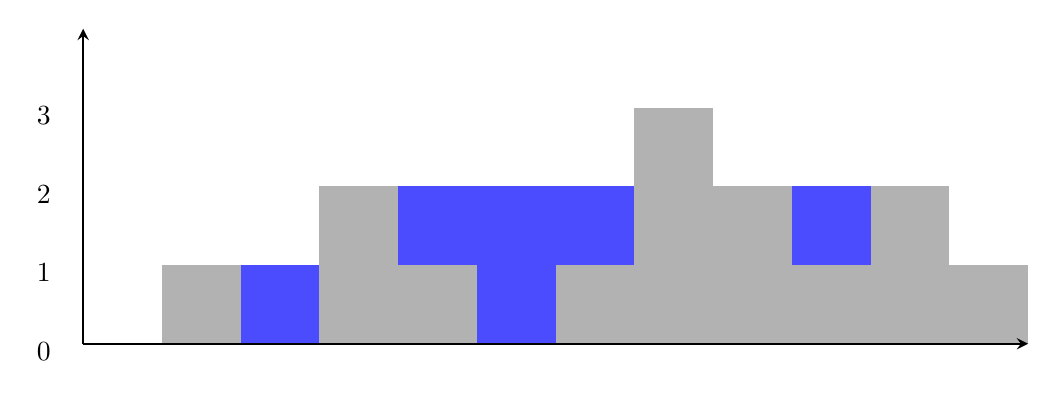
\begin{tikzpicture}
[thick, >=stealth, ->]
\draw (0,0) -- (0,4);
\node at (-0.5,0.9) {1}; 
\node at (-0.5,1.9) {2}; 
\node at (-0.5,2.9) {3};
 \node at (-0.5,-0.1) {0};
\fill[gray!60!] (1,0) rectangle ++(1,1);
\fill[gray!60!] (3,0) rectangle ++(1,2);
\fill[gray!60!] (4,0) rectangle ++(1,1);
\fill[gray!60!] (6,0) rectangle ++(1,1);
\fill[gray!60!] (7,0) rectangle ++(1,3);
\fill[gray!60!] (8,0) rectangle ++(1,2);
\fill[gray!60!] (9,0) rectangle ++(1,1);
\fill[gray!60!] (10,0) rectangle ++(1,2);
\fill[gray!60!] (11,0) rectangle ++(1,1);
\fill[blue!70!] (2,0) rectangle ++(1,1);
\fill[blue!70!] (4,1) rectangle (7,2);
\fill[blue!70!] (5,0) rectangle ++(1,1);
\fill[blue!70!] (9,1) rectangle ++(1,1);
\draw (0,0) -- (12,0);
\end{tikzpicture}
\end{figure}

The above elevation map is represented by array $[0,1,0,2,1,0,1,3,2,1,2,1]$. In this case, 6 units of rain water (blue section) are being trapped.


\paragraph{Example:}

\begin{flushleft}
\textbf{Input}: $[0,1,0,2,1,0,1,3,2,1,2,1]$

\textbf{Output}: 6
\end{flushleft}

\subsection{Stack}
\begin{itemize}
\item Maintain a stack $z$.
\item Traversing the input array. If current bar is no higher than the top element of the stack, which means that the current bar is bounded by the previous bar in the stack, we add index of current bar to $z$. Otherwise, pop the top from $z$ and add the trapped area to the result.
\item 理解上述算法的关键是,当pop出栈顶元素时,所形成的trapping water area其左边界就是当前的栈顶元素,而当前位置为右边界,所以计算trapping water 就要取左右边界最小的,然后减去之前弹出的栈顶元素的高度,即trapping water area底部的高度。
\end{itemize}

\setcounter{algorithm}{0}
\begin{algorithm}[H]
\caption{Stack}
\begin{algorithmic}[1]
\Procedure{Trap}{$H$, $n$}
\State $a:= 0$ \Comment Result trapping water area
\State $\star$ Maintain an empty stack $t$
\For{$i:=0$ \textbf{to} $n-1$}
\While{$t$ is not empty \textbf{and} $t_0 < H[i]$} \label{042while}
\State $\star$ Assign the top of $t$ to $x$, i.e. $x:=t_0$. 
\State $\star$ pop top $t_0$ from $t$
\If{$t$ is empty}
\State \textbf{break} \Comment Stack is empty so break loop [\ref{042while}]
\Else
\State $h := \min(H[t_0], H[i]) - H[x]$ \Comment Get the bounding height of the area
\State $d := i - t_0 - 1$ \Comment Get the length of the are
\State $a \gets a + h\times d$ \Comment Update total area.
\EndIf
\EndWhile
\EndFor
\State \Return $a$
\EndProcedure
\end{algorithmic}
\end{algorithm}

\setcounter{lstlisting}{0}
\begin{lstlisting}[style=customc, caption={Stack}]
int trap( vector<int>& height )
{
    stack<int> stk;

    int ans = 0;

    int L = static_cast<int>( height.size() );

    for( int i  = 0; i < L; ++i )
    {
        int h = height[i];

        while( !stk.empty() && ( height[stk.top()] <=  h ) )
        {
            int t = stk.top();
            stk.pop();

            if( stk.empty() )
            {
                break;
            }

            //the bounded rectangle height:
            //left boundary height: height[stk.top()]
            //right boundary height: height[t]
            int bound_h = ( min )( height[stk.top()], h ) - height[t];
            //the boundary rectangle length
            int bound_l = i - stk.top() - 1;

            ans += bound_h * bound_l;
        }

        stk.push( i );
    }

    return ans;

}
\end{lstlisting}

\subsection{Dynamic Programming}
The steps are listed as below
\begin{itemize}
\item Find maximum height of bar from the left up to an index $i$ into array $A_l$.
\item Find maximum height of bar from the right up to an index $i$ into the array $A_r$
\item Iterate over the height array and add the difference between $\min(A_l[i], A_r[i])$ and the height in current index to the answer.
\end{itemize}

\begin{algorithm}[H]
\caption{Dynamic Programming}
\begin{algorithmic}[1]
\Procedure{Trap}{$H$, $n$}
\State $a:= 0$ \Comment Result trapping water area
\State $\star$ Maintain an empty array $A_l$ with size $n$
\State $\star$ Maintain an empty array $A_r$ with size $n$
\State $\ast$ Fill $A_l$ and $A_r$
\State $A_l[0] = H[0]$
\State $A_r[n-1] = H[n-1]$
\For{$i:=1$ \textbf{to} $n-1$}
\State $\ast$ Fill $A_l$ from left to right
\State $A[i]\gets \max(H[i], A[i-1])$
\State $\ast$ Fill $A_r$ from right to left
\State $j = n - 1 -i$
\State $A[j]\gets \max(H[i], A[j+1])$
\EndFor
\State $\ast$ Get the total area
\For{$i:=0$ \textbf{to} $n-1$}
\State $a\gets a + \min(A_l[i], A_r[i]) - H[i]$
\EndFor
\State \Return $a$
\EndProcedure
\end{algorithmic}
\end{algorithm}

\setcounter{lstlisting}{0}
\begin{lstlisting}[style=customc, caption={Dynamic Programming}]
int trap( vector<int>& height )
{
    if( height.empty() )
    {
        return 0;
    }

    //l records maximum height so far from left to right
    vector<int> l( height.size(), 0 );
    //r records maximum height so far from right to left
    vector<int> r( height.size(), 0 );

    l[0] = height[0];
    r.back() = height.back();

    for( size_t i = 1; i < height.size(); ++i )
    {
        //fill l from left to right
        l[i] = ( max )( l[i - 1], height[i] );

        //fill r from right to left;
        auto j = height.size() - 1 - i;
        r[j] = ( max )( r[j + 1], height[j] );
    }

    int ans = 0;
    for( size_t i = 0; i < height.size(); ++i )
    {
        int h = ( min )( l[i], r[i] );
        //the difference between h and current height
        //is the water trapped in current bar
        ans += ( max )( h - height[i], 0 );
    }

    return ans;
}
\end{lstlisting}

\subsection{Two Pointers}
\begin{itemize}
\item 由于上述$A_l[i]$和$A_r[i]$只取决于$A_l[i-1]$,因此可以用两个变量$l$和$r$来代替。
\item 用左右两个index $x$ and $y$ 分别从left and right ends移动。如果 $H[x] < H[y]$,移动$x$,反之移动$y$。
\item $x$和$y$移动过程中,同时更新$l$ and $r$。
\end{itemize}


\begin{algorithm}[H]
\caption{Two Pointers}
\begin{algorithmic}[1]
\Procedure{Trap}{$H$, $n$}
\State $l:=0$ \Comment The maximum height from left to right so far
\State $r:=0$ \Comment The maximum height from right to left so far
\State $x:=0$ \Comment The left index
\State $y:=n-1$ \Comment The right index
\State $w:=0$ \Comment The total amount of trapped water
\While{$x < y$}
\If{$A[x] < A[y]$}
\State $\ast$ Move $x$ to right end
\State $l\gets \max(l, A[x])$ \Comment Update maximum height 
\State $w\gets w + (l-A[x])$ \Comment Add to total trapped water
\State $x\gets x+1$
\Else
\State $\ast$ Move $y$ to left end
\State $r\gets \max(r, A[y])$ \Comment Update maximum height 
\State $w\gets w + (r-A[y])$ \Comment Add to total trapped water
\State $y\gets y-1$
\EndIf
\EndWhile
\State \Return $w$
\EndProcedure
\end{algorithmic}
\end{algorithm}

\setcounter{lstlisting}{0}
\begin{lstlisting}[style=customc, caption={Two Pointers}]
int trap( vector<int>& height )
{
    int l = 0; //maximum height from left to right so far
    int r = 0; //maximum height from right to left so far

    int x = 0;
    int y = static_cast<int>( height.size() ) - 1;

    int ans = 0;

    while( x < y )
    {
        if( height[x] < height[y] )
        {
            //move x to right end
            l = ( max )( l, height[x] );
            ans += ( l - height[x] );
            ++x;
        }
        else
        {
            //move y to left end
            r = ( max )( r, height[y] );
            ans += ( r - height[y] );
            --y;
        }
    }

    return ans;
}
\end{lstlisting}
%\section{43 --- Multiply Strings}
Given two non-negative integers $A$ and $B$ represented as strings, return the product of $A$ and $B$, also represented as a string.

\paragraph{Example 1:}

\begin{flushleft}
\textbf{Input}: $A = 2$, $B = 3$

\textbf{Output}: 6
\end{flushleft}

\paragraph{Example 2:}

\begin{flushleft}
\textbf{Input}: $A = 123$, $B = 456$

\textbf{Output}: 56088
\end{flushleft}

\paragraph{Note:}

\begin{itemize}
\item The length of both $A$ and $B$ is less than 110.
\item Both $A$ and $B$ contain only digits $0--9$.
\item Both $A$ and $B$ do not contain any leading zero, except the number 0 itself.
\item You must not use any built-in \textbf{BigInteger} library or convert the inputs to integer directly.
\end{itemize}

\subsection{Mathematical Way}
\begin{itemize}
\item 需要一个额外的数组用来存放中间的运算过程。
\item 最后需要移除前面的零。
\end{itemize}


\setcounter{lstlisting}{0}
\begin{lstlisting}[style=customc, caption={Mathematical Way}]
string multiply( string num1, string num2 )
{
    size_t len_1 = num1.size();
    size_t len_2 = num2.size();

    //the maximum size of the product
    //is len_1 + len_2
    vector<int> product( len_1 + len_2, 0 );

    //reverse input numbers
    //so that the multiply is starting
    //from the beginning
    reverse( begin( num1 ), end( num1 ) );
    reverse( begin( num2 ), end( num2 ) );

    for( size_t i = 0; i < len_1; ++i )
    {
        for( size_t j = 0; j < len_2; ++j )
        {
            int v = ( num1[i] - '0' ) * ( num2[j] - '0' );

            product[i + j] += v;
            //accumulate the carry into next position
            product[i + j + 1] += product[i + j] / 10;
            //keep the number less than 10 in current position
            product[i + j] %= 10;
        }
    }

    //remove prefix zeros
    while( !product.empty() && ( product.back() == 0 ) )
    {
        product.pop_back();
    }

    if( product.empty() )
    {
        return "0";
    }

    string ans;

    //we need to reverse the array
    for( size_t i = 0; i < product.size(); ++i )
    {
        auto j = product.size() - 1 - i;
        ans.push_back( product[j] + '0' );
    }

    return ans;
}
\end{lstlisting}
%\section{44 --- Wildcard Matching}
Given an input string ($s$) and a pattern ($p$), implement wildcard pattern matching with support for $?$ and $\ast$.

\begin{itemize}
\item $?$ Matches any single character.
\item $\ast$ Matches any sequence of characters (including the empty sequence).
\item The matching should cover the entire input string (not partial).
\end{itemize}

\paragraph{Note:}

\begin{itemize}
\item $s$ could be empty and contains only lowercase letters $a--z$.
\item $p$ could be empty and contains only lowercase letters $a--z$, and characters like $?$ or $\ast$.
\end{itemize}

\paragraph{Example 1:}

\begin{flushleft}
\textbf{Input}: $s = \texttt{aa}$, $p = a$

\textbf{Output}: \texttt{false}

\textbf{Explanation}: $a$ does not match the entire string \texttt{aa}.
\end{flushleft}

\paragraph{Example 2:}

\begin{flushleft}
\textbf{Input}: $s = \texttt{aa}$, $p = \ast$

\textbf{Output}: \texttt{true}

\textbf{Explanation}: $\ast$ matches any sequence.
\end{flushleft}


\paragraph{Example 3:}

\begin{flushleft}
\textbf{Input}: $s = \texttt{cb}$, $p = ?a$

\textbf{Output}: \texttt{false}

\textbf{Explanation}: $?$ matches $c$, but the second letter is $a$, which does not match $b$.
\end{flushleft}


\paragraph{Example 4:}

\begin{flushleft}
\textbf{Input}: $s = \texttt{adceb}$, $p = \ast a\ast b$

\textbf{Output}: \texttt{true}

\textbf{Explanation}: The first $\ast$ matches the empty sequence, while the second $\ast$ matches the substring \texttt{dce}.

\end{flushleft}

\paragraph{Example 5:}

\begin{flushleft}
\textbf{Input}: $s = \texttt{acdcb}$, $p = a\ast c?b$

\textbf{Output}: \texttt{false}
\end{flushleft}

\subsection{Dynamic Programming}
\begin{itemize}
\item Define $F(i,j)$ as the match result of $s[0, i-1]$ with $p[0, j-1]$.
\item First, we need to fill the base cases, i.e. $F(0,i)$ for $i \in [0, m]$. This means when $s$ is empty, what is the match results of a empty string with $p[0, i-1]$. Apparently, only when $p[i-1] = \ast$, it may get result of true.
\item Then, starting the fill process. There will be two cases
\begin{enumerate}
\item if $p[j-1]=\ast$, $F(i,j) = F(i-1, j)$ \textbf{or} $F(i,j-1)$, i.e., either match $\ast$ with $s[i-1]$ (then the result will be coming from the match result of $s[0, i-2]$ with $p[0, j-1]$) or treat $\ast$ as nothing (then the result will be coming from the match result of $s[0,i-1]$ with $p[0,j-2]$)
\item if $p[j-1] = s[i-1]$ \textbf{or} $p[j-1] = ?$, $F(i,j) = F(i-1,j-1)$ (i.e the result will be coming from the match result of $s[0,i-2]$ and $p[0,j-2]$)
\end{enumerate}
\end{itemize}

\setcounter{algorithm}{0}
\begin{algorithm}[H]
\caption{Dynamic Programming}
\begin{algorithmic}[1]
\Procedure{IsMatch}{$S, n, P, m$}
\State $\star$ Create $F$ as an array filled zeros with size $(n+1)\times (m+1)$
\State $F[0][0]\gets 1$ \Comment empty string $s$ matches empty string $p$
\For{$i:=1$ \textbf{to} $m$}
\If{$P[i-1] = \ast$} \Comment Only $\ast$ can matches empty string $s$
\State $F[0][i] = F[0][i-1]$
\EndIf
\EndFor
\For{$i:=1$ \textbf{to} $n$}
\For{$j:=1$ \textbf{to} $m$}
\If{$P[j-1] = \ast$}
\State $F[i][j] = F[i-1][j]$ \textbf{or} $F[i][j-1]$
\ElsIf{$P[j-1] = ?$ \textbf{or} $S[i-1] = P[j-1]$}
\State $F[i][j] = F[i-1][j-1]$
\algstore{44algo}
\end{algorithmic}
\end{algorithm}
\begin{algorithm}[H]
\begin{algorithmic}[1]
\algrestore{44algo}
\EndIf
\EndFor
\EndFor
\If{$F[n][m] = 1$}
\State \Return \textbf{true} \Comment Matched
\Else
\State \Return \textbf{false} \Comment Not matched
\EndIf
\EndProcedure
\end{algorithmic}
\end{algorithm}

\setcounter{lstlisting}{0}
\begin{lstlisting}[style=customc, caption={Dynamic Programming}]
bool isMatch( string s, string p )
{
    auto m = s.size();
    auto n = p.size();

    vector<vector<int>> F( m + 1, vector<int>( n + 1, 0 ) );

    F[0][0] = 1; //empty vs empty

    for( size_t j = 1; j <= n; ++j )
    {
        if( p[j - 1] == '*' )
        {
            //only * can match empty string
            F[0][j] = F[0][j - 1];
        }
    }

    for( size_t i = 1; i <= m; ++i )
    {
        for( size_t j = 1; j <= n; ++j )
        {
            if( p[j - 1] == '*' )
            {
                //either treat * as s[i-1]
                F[i][j] = F[i - 1][j];
                //or treat * as nothing
                F[i][j] |= F[i][j - 1];
            }
            else if( ( p[j - 1] == '?' ) || ( p[j - 1] == s[i - 1] ) )
            {
                F[i][j] = F[i - 1][j - 1];
            }
        }
    }

    return F[m][n] == 1;
}
\end{lstlisting}
%\section{45 --- Jump Game II}
Given an array of non-negative integers $A$, you are initially positioned at the first index of the array.

Each element in the array represents your maximum jump length at that position.

Your goal is to reach the last index in the minimum number of jumps.

\paragraph{Example:}

\begin{flushleft}
\textbf{Input}: $[2,3,1,1,4]$

\textbf{Output}: 2

\textbf{Explanation}: 

The minimum number of jumps to reach the last index is 2. 

Jump 1 step from index 0 to 1, then 3 steps to the last index.
\end{flushleft}


\paragraph{Note:}

\begin{itemize}
\item You can assume that you can always reach the last index.
\end{itemize}


\subsection{BFS}
可以把每次所能到达的位置按照所需的jump数排成一个树状结构。例如,按照给定的例子,可以有如下的graph

%\begin{tikzpicture}[modal][H]
%\node[world] (2) [label=left:{level 0:}]{$2$};
%\node[world] (3) [label=left:{level 1:}, below = 2mm of 2]{$3$};
%\node[world] (1) [right = 2mm of 3]{$1$};
%\node[world] (11) [label=left:{level 2:}, below = 2mm of 3]{$1$};
%\node[world] (4) [right = 2mm of 11]{$4$};    
%\end{tikzpicture}
\begin{itemize}
\item 第0层就是位置为0的节点,它所能跳到的位置为1和2,也就是第1层的两个节点。
\item 第1层有位置为1和2的两个节点,其中位置1的节点,它能跳到位置2,3,4,而位置2已经在第1层了,所以第2层有位置3和4,位置2的节点,它能跳到位置3,所以第2层有位置3
\item 综合第1层的分析,第2层就有位置3和4的节点,而位置4已经是最后一个位置了,所以跳到4至少需要2步。
\end{itemize}

算法实现中,需要维护当前level所能跳到的最大位置,以及下一个level所能跳到的最大位置,然后遍历当前level,更新下一个level的最大位置,如果已经到达最后一个位置,就直接返回层数。

\setcounter{algorithm}{0}
\begin{algorithm}[H]
\caption{BFS}
\begin{algorithmic}[1]
\Procedure{Jump}{$A, n$}
\If{$n = 1$}
\State \Return 0 \Comment We already in the final position
\EndIf
\State $e_0 := 0$ \Comment The maximum position of current level
\State $e_1 := 0$ \Comment The maximum position of next level
\State $P:=0$ \Comment The current position
\State $\ell := 1$ \Comment We already in the zero level, next level will be level 1
\State $\ast$ Update next level's positions that can be reached
\While{$P \leq e_0$}
\State $e_1 \gets \max(e_1, A[P]+P)$ \Comment Update the maximum position of next level
\If{$e_1 \geq n-1$} \Comment Next level will contain the final position
\State \Return $\ell$
\EndIf
\If{$P = e_0$} \Comment Already in the end of current level
\State $e_0 \gets e_1$ \Comment Update as the maximum position of next level
\State $\ell\gets \ell+1$ \Comment Increments the number of levels
\EndIf
\State $P \gets P+1$ \Comment Move to next position
\EndWhile
\State \Return $\infty$ \Comment Cannot jump to the final position
\EndProcedure
\end{algorithmic}
\end{algorithm}

\setcounter{lstlisting}{0}
\begin{lstlisting}[style=customc, caption={BFS}]
int jump( vector<int>& nums )
{
    if( nums.size() == 1 )
    {
        return 0;
    }

    int L = static_cast<int>( nums.size() );

    int pos = 0;

    int cur_end = 0;
    int next_end = 0;

    //since current end is not the final end
    //we at least requires 1 jump
    int jumps = 1;

    while( pos <= cur_end )
    {
        next_end = ( max )( pos + nums[pos], next_end );

        if( next_end >= L - 1 )
        {
            //can jump to the final position
            return jumps;
        }
        if( pos == cur_end )
        {
            //move to next level
            cur_end = next_end;
            //increment the number of jumps
            ++jumps;
        }

        //test next position
        pos = pos + 1;
    }

    //cannot jump to final position
    return -1;
}
\end{lstlisting}
%\section{46 --- Permutations}
Given a collection of distinct integers $A$, return all possible permutations.

\paragraph{Example:}

\begin{flushleft}
\textbf{Input}: $[1,2,3]$

\textbf{Output}:

\begin{table}[H]
\begin{tabular}{ccc}
1 & 2 & 3\\
1 & 3 & 2\\
2 & 1 & 3\\
2 & 3 & 1\\
3 & 1 & 2\\
3 & 2 & 1
\end{tabular}
\end{table}
\end{flushleft}

\subsection{Backtracking By Setting Visited Status}
In this approach, when visit a number that does not visit before, mark its visited status as \texttt{true}. After recursive function ends, reset its visited status as \texttt{false}. In the recursive function, the loop will start from zero, since we need to enumerate all numbers.

\setcounter{algorithm}{0}
\begin{algorithm}[H]
\caption{Recursive With Visited Status}
\begin{algorithmic}[1]
\Procedure{Permute}{$A, n$}
\State $\star$ Create an empty array $v$ to save one permutation
\State $\star$ Create an empty array $\Phi$ for each number's visited status
\State $\star$ Create an empty array $P$ as the result.
\State \Call{DFS}{$A, n, \delta=0, v, \Phi, P$} 
\State \Return $P$
\EndProcedure
\end{algorithmic}
\end{algorithm}

The following function \texttt{DFS} recursively generate all permutations of input array $A$. The result is $P$, while $\Phi$ is for recording each number's visited status. $\delta$ is the count of numbers that have been visited.
\begin{algorithm}[H]
\caption{Helper function}
\begin{algorithmic}[1]
\Function{DFS}{$A, n, \delta, v, \Phi, P$}
\If{$\delta = n$} \Comment Iterate all elements in $A$
\State $\star$ Add $v$ into the final list
\Else
\For{$i:=0$ \textbf{to} $n-1$}
\If{$\Phi[i] = 1$} \Comment $A[i]$ has been visited
\State \texttt{continue} \Comment Skip this number
\EndIf
\State $\Phi[i] \gets 1$ \Comment Mark $A[i]$ as visited
\State $v \gets v + A[i]$ \Comment Add $A[i]$ into $V$
\State \Call{DFS}{$A, n, \delta=\delta+1, v, \Phi, P$} \Comment Recursively generate permutation from next number
\State $v \gets v - A[i]$ \Comment Remove $A[i]$ from $v$
\State $\Phi[i] \gets 0$ \Comment Reset $A[i]$ as not visited
\EndFor
\EndIf
\EndFunction
\end{algorithmic}
\end{algorithm}

\setcounter{lstlisting}{0}
\begin{lstlisting}[style=customc, caption={Recursive With Visited Status}]
vector<vector<int>> permute( vector<int>& nums )
{
    vector<int> seen( nums.size(), 0 );

    vector<int> cur; //save current permutation result

    cur.reserve( nums.size() );

    vector<vector<int>> ans;

    dfs( nums, seen, cur, ans );

    return ans;
}

//helper function for recursion
void dfs( const vector<int>& A, vector<int>& seen, vector<int>& cur, vector<vector<int>>& ans )
{
    if( cur.size() == A.size() )
    {
        //all numbers have been visited
        ans.emplace_back( cur.begin(), cur.end() );
        return;
    }

    for( size_t i = 0; i < A.size(); ++i )
    {
        if( seen[i] )
        {
            continue;
        }

        seen[i] = 1;
        cur.push_back( A[i] );

        dfs( A, seen, cur, ans );

        //backtrack
        seen[i] = 0;
        cur.pop_back();
    }
}
\end{lstlisting}

\subsection{Backtracking By Swapping}
\begin{itemize}
\item In this approach, we swap the current first item $A[p]$ with each number starting from position $p$. 
\item If starting from position $p+1$, we will miss the arrays that start with $A[p]$
\end{itemize}


\begin{algorithm}[H]
\caption{Backtrack With Swap}
\begin{algorithmic}[1]
\Procedure{Permute}{$A,n$}
\State $\star$ Create an empty array $\Omega$ as the result.
\State \Call{DFS}{$A, n, p=0, \Omega$} 
\State \Return $P$
\EndProcedure
\end{algorithmic}
\end{algorithm}


The following helper function \texttt{DFS2} swap $A[p]$ with each number starting from index $p$ and recursively going to next number.

\begin{algorithm}[H]
\caption{Helper Function}
\begin{algorithmic}[1]
\Function{DFS2}{$A, n, p, \Omega$}
\If{$p = n$} \Comment All numbers are permutated once
\State $\star$ Add current $A$ into result list $\Omega$
\State \Return
\Else
\For{$i:= p$ \textbf{to} $n-1$}
\State $\star$ Swap $A[p]$ with $A[i]$ 
\State \Call{DFS2}{$A, n, p = p+1, \Omega}$ \Comment Generate permutation starting with $A[p+1]$
\State $\star$ Swap $A[p]$ with $A[i]$ to backtrack 
\EndFor
\EndIf
\EndFunction
\end{algorithmic}
\end{algorithm}

\setcounter{lstlisting}{0}
\begin{lstlisting}[style=customc, caption={Backtrack With Swap}]
vector<vector<int>> permute( vector<int>& nums )
{
    vector<vector<int>> ans;

    dfs( nums, 0, ans );

    return ans;
}
//Helper function to generate permutation lists
void dfs( vector<int>& A, size_t start, vector<vector<int>>& ans )
{
    if( start == A.size() )
    {
        ans.emplace_back( A.begin(), A.end() );
        return;
    }

    for( size_t i = start; i < A.size(); ++i )
    {
        swap( A[i], A[start] );

        //permut starting from A[start+1]
        dfs( A, start + 1, ans );

        //swap back to backtrack
        swap( A[i], A[start] );
    }
}
\end{lstlisting}

%\section{47 --- Permutations II}

Given a collection of numbers that might contain duplicates $A$, return all possible unique permutations.

\paragraph{Example:}

\begin{flushleft}
\textbf{Input}: $[1,1,2]$

\textbf{Output}:

\begin{table}[H]
\begin{tabular}{ccc}
1 & 1 & 2\\
1 & 2 & 1\\
2 & 1 & 1
\end{tabular}
\end{table}
\end{flushleft}

\subsection{Backtracking By Setting Visited Status}
\begin{itemize}
\item 由于输入数组有可能出现重复数字,如果按照之前的算法,会有重复排列产生,
\item 要避免重复的产生,首先要对原数列进行排序,
\item 然后在递归函数中要判断前面一个数和当前的数是否相等,如果相等,当前面的数已经使用了,当前的数字才能使用,否则需要跳过,这样就不会产生重复排列了
\end{itemize}

\setcounter{algorithm}{0}
\begin{algorithm}[H]
\caption{Backtracking With Visited Status}
\begin{algorithmic}[1]
\Procedure{Permute}{$A, n$}
\State $\star$ Create $\Omega$ as the result list
\State Sort $A$ by ascending order
\State $\star$ Create $\Phi$ to record each number's visited status
\State $\star$ Create $v$ to store one permutation result
\State \Call{DFS}{$A, n, v, \Phi, \Omega$} 
\State \Return $\Omega$
\EndProcedure
\end{algorithmic}
\end{algorithm}

The following function \texttt{DFS} generates unique permutations for input array $A$.
\begin{algorithm}[H]
\caption{Backtracking Helper Function}
\begin{algorithmic}[1]
\Function{DFS}{$A,n,v, \Phi,\Omega$}
\If{$\lvert v\rvert = n$} \Comment All elements in $A$ are in $v$
\State $\star$ Add $v$ to result list $\Omega$
\State \Return
\EndIf
\For{$i:=0$ \textbf{to} $n-1$}
\If{$\Phi[i] = 1$} \Comment $A[i]$ has been visited
\State \texttt{continue} \Comment Skip this number
\EndIf
\If{$i > 0$ \textbf{and} $A[i-1] = A[i]$ \textbf{and} $\Phi[i-1] = 0$}
\State \texttt{continue} \Comment Skip duplicate and yet not visited elements
\EndIf
\State $\Phi[i] \gets 1$ \Comment Mark $A[i]$ as visited
\State $v \gets v + A[i]$ \Comment Add $A[i]$ into $v$
\State $\ast$ Recursively generate permutation for next level
\State \Call{DFS}{$A, n, v, \Phi, \Omega$}
\State $\ast$ Restore state for backtracking
\State $\Phi[i] \gets 0$ \Comment Mark $A[i]$ as not visited
\State $v \gets v - A[i]$ \Comment Remove $A[i]$ into $v$
\EndFor
\EndFunction
\end{algorithmic}
\end{algorithm}

\setcounter{lstlisting}{0}
\begin{lstlisting}[style=customc, caption={Backtracking By Setting Visited Status}]
vector<vector<int>> permuteUnique( vector<int>& nums )
{
    //nums must be sorted
    sort( begin( nums ), end( nums ) );

    vector<int> seen( nums.size(), 0 );

    vector<vector<int>> ans;

    vector<int> v;
    v.reserve( nums.size() );

    dfs( nums, v, seen, ans );

    return ans;
}

//helper function to generate unique permutation
void dfs( const vector<int>& A,
          vector<int>& v,
          vector<int>& seen,
          vector<vector<int>>& ans )
{
    if( v.size() == A.size() )
    {
        ans.emplace_back( v.begin(), v.end() );
        return;
    }

    for( size_t i = 0; i < A.size(); ++i )
    {
        if( seen[i] == 1 )
        {
            //A[i] has been visited
            continue;
        }

        if( ( i > 0 ) && ( A[i - 1] == A[i] ) && ( seen[i - 1] == 0 ) )
        {
            //skip duplicate
            //that has not been visited
            continue;
        }

        seen[i] = 1;
        v.push_back( A[i] );

        dfs( A, v, seen, ans );

        seen[i] = 0;
        v.pop_back();
    }
}
\end{lstlisting}
%\section{48 --- Rotate Image}
You are given an $n \times n$ 2D matrix representing an image.

Rotate the image by 90 degrees (clockwise).

\paragraph{Note:}

\begin{itemize}
\item You have to rotate the image in-place, which means you have to modify the input 2D matrix directly. \textbf{DO NOT} allocate another 2D matrix and do the rotation.
\end{itemize}

\paragraph{Example 1:}
\begin{flushleft}
\textbf{Input}:
\begin{table}[H]
\begin{tabular}{ccc}
1 & 2 & 3\\
4 & 5 & 6\\
7 & 8 & 9
\end{tabular}
\end{table}
\textbf{Output}:
\begin{table}[H]
\begin{tabular}{ccc}
7 & 4 & 1\\
8 & 5 & 2\\
9 & 6 & 3
\end{tabular}
\end{table}
\end{flushleft}

\paragraph{Example 2:}
\begin{flushleft}
\textbf{Input}:
\begin{table}[H]
\begin{tabular}{cccc}
5 &  1 &  9 & 11\\
2 &  4 &  8 & 10\\
13 &  3 &  6 &  7\\
15 & 14 & 12 & 16
\end{tabular}
\end{table}
\textbf{Output}:
\begin{table}[H]
\begin{tabular}{cccc}
15 & 13 &  2 &  5\\
14 &  3 &  4 &  1\\
12 &  6 &  8 &  9\\
16 &  7 & 10 & 11
\end{tabular}
\end{table}
\end{flushleft}

\subsection{Transpose and then reverse}
\begin{enumerate}
\item The obvious idea would be to transpose the matrix first and then reverse each row. 
\end{enumerate}

\setcounter{lstlisting}{0}
\begin{lstlisting}[style=customc, caption={Transpose Then Reverse}]
void rotate( vector<vector<int>>& matrix )
{
    int n = static_cast<int>( matrix.size() );

    //transpose
    for( int x = 0; x < n; ++x )
    {
        //notice each column starting
        //from x
        for( int y = x; y < n; ++y )
        {
            swap( matrix[x][y], matrix[y][x] );
        }
    }

    //reverse each row

    for( int x = 0; x < n; ++x )
    {
        reverse( matrix[x].begin(), matrix[x].end() );
    }

}
\end{lstlisting}

\subsection{Rotate four numbers}
每次移动4个数字

\setcounter{lstlisting}{0}
\begin{lstlisting}[style=customc, caption={Rotate 4 Numbers Each Time}]
void rotate( vector<vector<int>>& matrix )
{
    auto n = matrix.size();

    //move 4 number at each time
    for( size_t x = 0; x < n / 2; ++x )
    {
        for( size_t y = x; y < n - 1 - x; ++y )
        {
            int tmp = matrix[x][y];
            //overwrite top left by bottom left
            matrix[x][y] = matrix[n - 1 - y][x];
            //overwrite bottom left by bottom right
            matrix[n - 1 - y][x] = matrix[n - 1 - x][n - 1 - y];
            //overwrite bottom right by top right
            matrix[n - 1 - x][n - 1 - y] = matrix[y][n - 1 - x];
            //overwrite top right by value from top left
            matrix[y][n - 1 - x] = tmp;
        }
    }
}
\end{lstlisting}
%\section{49 --- Group Anagrams}
Given an array of strings $A$, group anagrams together.

\paragraph{Example:}
\begin{flushleft}

\textbf{Input}: [eat, tea, tan, ate, nat, bat]


\textbf{Output}:

\begin{table}[H]
\begin{tabular}{lll}
ate & eat & tea \\
nat & tan & \\
bat & &
\end{tabular}
\end{table}

\end{flushleft}
\paragraph{Note:}

\begin{itemize}
\item All inputs will be in lowercase.
\item The order of your output does not matter.
\end{itemize}

\subsection{Counting Sort}
\begin{itemize}
\item 遍历输入字符串数组,对每一个字符串$S$,用一个大小为26的数组来统计每个单词中字符出现的次数,然后按照从$a$--$z$的顺序来组成一个字符串作为hash map的key。
\item 为了优化,hash map的value是存放每个字符串在字符串数组中的index。
\end{itemize}

\setcounter{lstlisting}{0}
\begin{lstlisting}[style=customc, caption={Counting Sort}]
vector<vector<string>> groupAnagrams( vector<string>& strs )
{
    //optimize memory and runtime performance
    //use array of index as the value of the
    //hash map
    unordered_map<string, vector<size_t>> m;

    int chars[26] = {0};

    for( size_t i = 0; i < strs.size(); ++i )
    {
        const auto&str = strs[i];

        for( auto c : str )
        {
            chars[c - 'a'] += 1;
        }

        string key;

        //contruct the key
        for( int i = 0; i < 26; ++i )
        {
            key.append( chars[i], i + 'a' );
            chars[i] = 0;
        }

        auto it = m.find( key );

        if( it == m.end() )
        {
            m.emplace( key, initializer_list<size_t> {i} );
        }
        else
        {
            it->second.emplace_back( i );
        }
    }

    vector<vector<string>> ans( m.size() );

    size_t j = 0;

    for( const auto&p : m )
    {
        for( size_t i : p.second )
        {
            ans[j].emplace_back( strs[i].c_str() );
        }

        ++j;
    }

    return ans;
}
\end{lstlisting}
%\section{50 --- Pow(x, n)}
Implement \texttt{pow}($x, n$), which calculates $x$ raised to the power $n$ ($x^n$).

\paragraph{Example 1:}

\begin{flushleft}
\textbf{Input}: $2.00000, 10$

\textbf{Output}: $1024.00000$
\end{flushleft}

\paragraph{Example 2:}

\begin{flushleft}
\textbf{Input}: $2.10000, 3$

\textbf{Output}: $9.26100$
\end{flushleft}

\paragraph{Example 3:}

\begin{flushleft}
\textbf{Input}: $2.00000, -2$

\textbf{Output}: $0.25000$

\textbf{Explanation}: $2^{-2} = 1/2^2 = 1/4 = 0.25$
\end{flushleft}


\paragraph{Note:}

\begin{itemize}
\item $-100.0 < x < 100.0$
\item $n$ is a 32-bit signed integer, within the range $[−2^{31}, 2^{31} − 1]$
\end{itemize}

\subsection{Divide And Conquer}
The most difficult is dealing with maximum integer type and minimum integer type. Therefore, we need to compute the result of half of the exponent at the first time.
\setcounter{algorithm}{0}
\begin{algorithm}[H]
\caption{Divide And Conquer}
\begin{algorithmic}[1]
\Procedure{MyPow}{$x, n$}
\If{$n = 0$}
\State \Return 1 \Comment $x^0 = 1$
\EndIf
\State $\alpha :=$ \Call{MyPow}{$x, n/2$} \Comment Get $x^{n/2}$
\algstore{50algo}
\end{algorithmic}
\end{algorithm}
\begin{algorithm}[H]
\begin{algorithmic}[1]
\algrestore{50algo}
\If{$n \bmod 2 = 0$}
\State \Return $\alpha^2$ \Comment $x^n = x^{n/2} \times x^{n/2}$
\ElsIf{$n > 0$}
\State \Return $\alpha^2\times x$ \Comment $x^n = {x^{n/2}}^2\times x$
\Else
\State \Return $\alpha^2 / x$ \Comment $x^n = {x^{n/2}}^2 / x$
\EndIf
\EndProcedure
\end{algorithmic}
\end{algorithm}

\setcounter{lstlisting}{0}
\begin{lstlisting}[style=customc, caption={Divide And Conquer}]
double myPow( double x, int n )
{

    //convert to long long type
    //to avoid data type overflow
    auto exp = static_cast<long long>( n );

    if( exp >= 0 )
    {

        return f( x, exp );
    }

    exp *= -1;
    return 1 / f( x, exp );
}

double f( double x, long long n )
{
    if( n == 0 )
    {
        return 1;
    }

    if( n == 1 )
    {
        return x;
    }

    auto exp = n / 2;
    auto y = f( x, exp );

    y *= y;

    if( n & 1 )
    {
        //odd exponent
        return x * y;
    }

    return y;
}
\end{lstlisting}


\subsection{Iterative Method}
假设需要计算$x^{13}$。
\begin{itemize}
\item 13的二进制为$1101$。由于有4个bits,所以需要4 iterations。
\item First, initialize the result to 1: $r\gets 1 = x^0$。然后从左到右扫描bits
\begin{enumerate}
\item $r\gets r^2 = x^0$, bit 1 is 1, so $r\gets r\times x = x^1$
\item $r\gets r^2 = x^2$, bit 2 is 0, so $r\gets r\times x = x^3$
\item $r\gets r^2 = x^6$, bit 3 is 0, so $r\gets r\times x^0 = x^6$
\item $r\gets r^2 = x^{12}$, bit 4 is 1, so $r\gets r\times x = x^{13}$
\end{enumerate} 
\end{itemize}
\begin{algorithm}[H]
\caption{Iterative Method}
\begin{algorithmic}[1]
\Procedure{MyPow}{$x,n$}
\State $r := 1$ \Comment $r = x^n$ 
\State $i:=n$
\While{$i \neq 0$}
\If{$i \bmod 2 = 1$}
\State $r \gets r \times x$
\EndIf
\State $x\gets x^2$
\State $i \gets i / 2$
\EndWhile
\If{$n < 0$}
\State \Return $1/r$
\Else
\State \Return $r$
\EndIf
\EndProcedure
\end{algorithmic}
\end{algorithm}

\setcounter{lstlisting}{0}
\begin{lstlisting}[style=customc, caption={Iterative}]
double myPow( double x, int n )
{
    double r = 1.0;
    auto i = static_cast<long long>( n );

    if( i < 0 )
    {
        i = -i;
    }

    while( i )
    {

        if( i & 1 )
        {
            //multiply x
            //for bit 1
            r *= x;
        }

        //always do x<--x*x
        x *= x;

        i /= 2;
    }

    if( n < 0 )
    {
        return 1 / r;
    }

    return r;
}
\end{lstlisting}

%\section{51 --- N-Queens}
The $n$-queens puzzle is the problem of placing $n$ queens on an $n\times n$ chessboard such that no two queens attack each other.


Given an integer $n$, return all distinct solutions to the $n$-queens puzzle.

Each solution contains a distinct board configuration of the n-queens' placement, where \texttt{Q} and dot both indicate a queen and an empty space respectively.

\subsection{Backtrack}
\begin{itemize}
\item There could be the only one queen in a row and the only one queen in a column. This means that there is no need to consider all squares on the board. One could just iterate over the columns.
\item For all diagonals the sum of row and column of each square is constant
\item For all anti-diagonals the difference between row and column of each square is constant.
\end{itemize}

The backtrack algorithm is listed as below

\setcounter{algorithm}{0}
\begin{algorithm}[H]
\caption{$N$-Queen Backtarck}
\begin{algorithmic}[1]
\Procedure{Backtrack}{$n$}
\State $\star$ Start from the first $r = 0$.
\State $\star$ Iterate over the columns and try to put a queen in each column.
\If{Square $(r,c)$ is not under attack}
\State $\star$ Place the queen in $(r, c)$ square.
\State Exclude one row, one column and two diagonals from further consideration.
\If{$r = n$} \Comment All rows are filed up
\State $\star$ One solution is found
\Else
\State \Call{Backtrack}{$n+1$} \Comment Proceed to place further queens 
\EndIf
\State $\star$ Now backtrack, remove the queen from $(r,c)$.
\EndIf
\EndProcedure
\end{algorithmic}
\end{algorithm}

\setcounter{lstlisting}{0}
\begin{lstlisting}[style=customc, caption={Backtrack}]
vector<vector<string>> solveNQueens( int n )
{
    vector<int> queens( n );

    vector<unsigned char> rows( n, 0 );
    vector<unsigned char> hills( 2 * n - 1, 0 );
    vector<unsigned char> dales( 2 * n - 1, 0 );

    vector<vector<string>> ans;

    dfs( 0, n, rows, hills, dales, queens, ans );

    return ans;
}

void dfs( int r, int n,
          vector<unsigned char>& rows,
          vector<unsigned char>& hills,
          vector<unsigned char>& dales,
          vector<int>& queens,
          vector<vector<string>>& ans )
{
    for( int c = 0; c < n; ++c )
    {
        if( hills[r + c] + dales[r - c + n - 1] + rows[c] == 0 )
        {
            //place queen at (r,c)
            queens[r] = c;
            hills[r + c] = 1;
            dales[r - c + n - 1] = 1;
            rows[c] = 1;

            if( r + 1 == n )
            {
                //we have filled all rows
                vector<string> chess( n, string( n, '.' ) );

                for( int i = 0; i < n; ++i )
                {
                    chess[i][queens[i]] = 'Q';
                }

                ans.push_back( move( chess ) );
            }
            else
            {
                //depth first search
                dfs( r + 1, n, rows, hills, dales, queens, ans );
            }

            //backtrack
            queens[r] = 0;
            hills[r + c] = 0;
            dales[r - c + n - 1] = 0;
            rows[c] = 0;
        }
    }
}
\end{lstlisting}
%\section{52 --- N-Queens II}
The $n$-queens puzzle is the problem of placing $n$ queens on an $n\times n$ chessboard such that no two queens attack each other.

Given an integer $n$, return the number of distinct solutions to the $n$-queens puzzle.

\subsection{Backtrack}

\begin{itemize}
\item Almost same as Problem 51. The only difference in this problem, we just count the total possible placements.
\end{itemize}

\setcounter{lstlisting}{0}
\begin{lstlisting}[style=customc, caption={Backtrack}]
int totalNQueens( int n )
{
    vector<int> queens( n );

    vector<unsigned char> rows( n, 0 );
    vector<unsigned char> hills( 2 * n - 1, 0 );
    vector<unsigned char> dales( 2 * n - 1, 0 );

    int ans = 0;

    dfs( 0, n, rows, hills, dales, queens, ans );

    return ans;
}

void dfs( int r, int n,
          vector<unsigned char>& rows,
          vector<unsigned char>& hills,
          vector<unsigned char>& dales,
          vector<int>& queens,
          int& ans )
{
    for( int c = 0; c < n; ++c )
    {
        if( hills[r + c] + dales[r - c + n - 1] + rows[c] == 0 )
        {
            //place queen at (r,c)
            queens[r] = c;
            hills[r + c] = 1;
            dales[r - c + n - 1] = 1;
            rows[c] = 1;

            if( r + 1 == n )
            {
                //all queens are placed
                //increments the result
                ++ans;
            }
            else
            {
                //try next row
                dfs( r + 1, n, rows, hills, dales, queens, ans );
            }

            //backtrack
            queens[r] = 0;
            hills[r + c] = 0;
            dales[r - c + n - 1] = 0;
            rows[c] = 0;
        }
    }
}
\end{lstlisting}
%\section{53 --- Maximum Subarray}
Given an integer array $A$, find the contiguous subarray (containing at least one number) which has the largest sum and return its sum.
\paragraph{Example:}
\begin{flushleft}
\textbf{Input}: $[-2,1,-3,4,-1,2,1,-5,4]$,
\\
\textbf{Output}: 6
\\
\textbf{Explanation}: 
\\
$[4,-1,2,1]$ has the largest sum 6.
\end{flushleft}

\paragraph{Follow up:}
\begin{flushleft}
If you have figured out the $O(n)$ solution, try coding another solution using the divide and conquer approach, which is more subtle.
\end{flushleft}

\subsection{Kadane Algorithm}
\setcounter{algorithm}{0}
\begin{algorithm}[H]
\caption{Kadane Algorithm}
\begin{algorithmic}[1]
\Procedure{MaxSubArray}{$A$, $n$}
\State $\alpha := A[0]$ \Comment Current maximum
\State $\beta:=A[0]$ \Comment Maximum So far
\For{$i:=1$ \textbf{to} $n-1$}
\State $\alpha \gets A[i] + \max(\alpha, 0)$
\State $\beta \gets \max(\beta, \alpha)$
\EndFor
\State \Return $\beta$
\EndProcedure
\end{algorithmic}
\end{algorithm}

\setcounter{lstlisting}{0}
\begin{lstlisting}[style=customc, caption={Kadane Algorithm}]
int maxSubArray( vector<int>& nums )
{
    int cur_max = nums[0];
    int global_max = nums[0];

    for( size_t i = 1; i < nums.size(); ++i )
    {
        cur_max = nums[i] + ( max )( cur_max, 0 );
        global_max = ( max )( global_max, cur_max );
    }

    return global_max;
}
\end{lstlisting}

\subsection{Divide And Conquer}
The problem is a classical example of divide and conquer approach, and can be solved with the algorithm similar with the merge sort.

The solution template for the divide and conquer problems is as follows:

\begin{itemize}
\item Define the base case(s).

\item Split the problem into subproblems and solve them recursively.

\item Merge the solutions for the subproblems to obtain the solution for the original problem.
\end{itemize}

应用到这个问题中,算法如下:

\begin{enumerate}
\item Base case: if $n=\lvert A\rvert=1$, return $A[0]$
\item Get result $l$ for left sub-array, i.e., the first $n/2$ elements.
\item Get result $r$ for right sub-array, i.e., the last $n/2$ elements.
\item Get result $c$ that crossing the middle point.
\item Merge the solutions above, i.e, return $\max(l, r, c)$
\end{enumerate}

\begin{lstlisting}[style=customc, caption={Divide And Conquer}]
int maxSubArray( vector<int>& nums )
{
    int n = static_cast<int>( nums.size() );
    return f( nums, 0, n - 1 );
}

//helper function for recursion
int f( vector<int>& nums, int low, int high )
{
    if( low == high )
    {
        //base case:
        return nums[low];
    }

    int middle = ( low + high ) / 2;

    //find left half result
    int l = f( nums, low, middle );
    //find right half result
    int r = f( nums, middle + 1, high );
    //find cross sum
    int c = max_crossing_sum( nums, low, high, middle );

    //return the maximum result of (l, r, c)
    int x = ( max )( l, r );
    x = ( max )( x, c );
    return x;
}

//get maximum sum cross the middle point
int max_crossing_sum( vector<int>& A, int low, int high, int middle )
{
    //get maximum sum in [low,middle]
    int left_sum = INT_MIN;
    int sum = 0;

    for( int i = middle; i >= low; --i )
    {
        sum += A[i];
        left_sum = ( max )( sum, left_sum );
    }

    //get maximum sum in [middle+1, high]
    int right_sum = INT_MIN;
    sum = 0;
    int max_right = middle;

    for( int k = middle + 1; k <= high; ++k )
    {
        sum += A[k];
        right_sum = ( max )( sum, right_sum );
    }

    //combine the two sum
    return left_sum + right_sum;
}
\end{lstlisting}
%\section{54 --- Spiral Matrix}
Given a matrix of $m \times n$ elements ($m$ rows, $n$ columns), return all elements of the matrix in spiral order.
\paragraph{Example 1:}
\begin{flushleft}
\textbf{Input}:
\begin{figure}[H]
    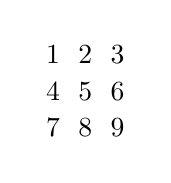
\begin{tikzpicture}
    \matrix [matrix of nodes]
    {
        1 & 2 & 3 \\
        4 & 5 & 6 \\
        7 & 8 & 9\\
    };
    \end{tikzpicture}
\end{figure}
\par
\textbf{Output}: $[1,2,3,6,9,8,7,4,5]$
\end{flushleft}
\paragraph{Example 2:}
\begin{flushleft}
\textbf{Input}:
\par
\begin{figure}[H]
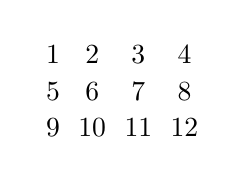
\begin{tikzpicture}
    \matrix [matrix of nodes]
    {
          1 & 2 & 3 & 4\\
          5 & 6 & 7 & 8\\
          9 & 10 & 11 & 12 \\
    };
\end{tikzpicture}
\end{figure}
\par
\textbf{Output}: $[1,2,3,4,8,12,11,10,9,5,6,7]$
\end{flushleft}

\subsection{Simulation}
Draw the path that the spiral makes. We know that the path should turn clockwise whenever it would go out of bounds or into a cell that was previously visited.
\par
Suppose the matrix $M$ have $R$ rows and $C$ columns. $\nu[r][c]$ is a $0/1$ auxiliary matrix denotes that the cell on the $r$-th row and $c$-th column was previously visited. Our current position is $(r_0, c_0)$, facing direction $\theta$, and we want to visit $R\times C$ total cells.
\par
As we move through the matrix, our candidate next position is $(r_1, c_1)$. If the candidate is in the bounds of the matrix and not seen before, i.e. not in $\nu$, then it becomes our next position; otherwise, our next position is the one after performing a clockwise turn.

The input parameter includes the matrix $A$, number of rows $R$ and number of columns $C$. The return value is array $\phi$, the elements that visited through spiral order.


\setcounter{lstlisting}{0}
\begin{lstlisting}[style=customc, caption={Simulation}]
vector<int> spiralOrder( vector<vector<int>>& matrix )
{
    if( matrix.empty() || matrix[0].empty() )
    {
        return {};
    }

    vector<vector<unsigned char>> seen( matrix.size(), vector<unsigned char>( matrix[0].size(), 0 ) );

    //the sequence cannot be
    //changed.
    int dr[] = {0, 1, 0, -1};
    int dc[] = {1, 0, -1, 0};

    vector<int> ans;

    int r = 0;
    int c = 0;
    //direction
    int d = 0;

    int rows = static_cast<int>( matrix.size() );
    int cols = static_cast<int>( matrix[0].size() );
    int total = static_cast<int>( rows * cols );

    ans.reserve( total );

    for( int i = 0; i < total; ++i )
    {
        ans.push_back( matrix[r][c] );
        seen[r][c] = 1;

        int nr = r + dr[d];
        int nc = c + dc[d];

        if( ( nr >= 0 ) && ( nr < rows ) && ( nc >= 0 ) && ( nc < cols ) && ( !seen[nr][nc] ) )
        {
            //(nr,nc) is inside range
            //and (nr,nc) has not seen
            r = nr;
            c = nc;
        }
        else
        {
            //change the direction
            d = ( ( d + 1 ) % 4 );
            r += dr[d];
            c += dc[d];
        }
    }

    return ans;
}
\end{lstlisting}

%\section{55 --- Jump Game}
Given an array of non-negative integers, $A$, you are initially positioned at the first index of the array.

Each element in the array represents your maximum jump length at that position.

Determine if you are able to reach the last index.

\paragraph{Example 1:}

\begin{flushleft}
\textbf{Input}: $[2,3,1,1,4]$

\textbf{Output}: \texttt{true}

\textbf{Explanation}: Jump 1 step from index 0 to 1, then 3 steps to the last index.

\end{flushleft}

\paragraph{Example 2:}

\begin{flushleft}
\textbf{Input}: $[3,2,1,0,4]$

\textbf{Output}: \texttt{false}

\textbf{Explanation}: 

You will always arrive at index 3 no matter what. Its maximum jump length is 0, which makes it impossible to reach the last index.
\end{flushleft}


\subsection{Graphic Level Equivalent}
和45题Jump Game II解法基本一致,同样将其看作是多个level的图, $\alpha_0$表示当前level的ending position,$\alpha_1$为下个level的ending position。遍历当前level中的each position,更新下个level的ending position。一旦当前位置到达$\alpha_0$,即表示进入下一个level了,那么$\alpha_0$更新为$\alpha_1$

\setcounter{lstlisting}{0}
\begin{lstlisting}[style=customc, caption={Graphic Approach}]
bool canJump( vector<int>& nums )
{
    //current level end position
    int cur_end = 0;
    //next level end position
    int next_end = 0;

    int p = 0;

    int L = static_cast<int>( nums.size() );

    while( p <= cur_end )
    {
        //update next level end position
        next_end = ( max )( next_end, p + nums[p] );

        if( next_end >= L - 1 )
        {
            return true;
        }

        if( p == cur_end )
        {
            cur_end = next_end;
        }

        ++p;
    }

    return false;
}
\end{lstlisting}

\subsection{Dynamic Programming Top-down}
Top-down Dynamic Programming can be thought of as optimized backtracking. It relies on the observation that once we determine that a certain index is good / bad, this result will never change. This means that we can store the result and not need to recompute it every time.

Therefore, for each position in the array, we store whether the index is good or bad into an array, say $M$ and let its values be either one of: \texttt{GOOD}, \texttt{BAD} or \texttt{UNKNOWN}.

Then, the steps of the algorithm are 
\begin{enumerate}
\item Initially, all elements of the memo table are \texttt{UNKNOWN}, except for the last one, which is \texttt{GOOD} (it can reach itself)
\item First checks if a index $i$ is known (\texttt{GOOD} / \texttt{BAD})
\begin{itemize}
\item If it is known then return the stored result.
\item Otherwise perform the DFS and backtracking steps.
\end{itemize}
\item Once we determine the value of the current index, we store it in the $M$
\end{enumerate}

However, this approach will cause \textbf{TLE}.

\begin{lstlisting}[style=customc, caption={Top Down Dynamic Programming}]
//This will cause TLE
//only for reference
bool canJump( vector<int>& nums )
{

    if( nums.empty() || ( nums.size() == 1 ) )
    {
        return true;
    }

    vector<unsigned char> memo( nums.size(), 0 );

    memo.back() = 2; //Good

    return dfs( nums, 0, memo );
}
//recursive helper function
bool dfs( vector<int>& A, size_t start, vector<unsigned char>& memo )
{
    if( memo[start] > 0 )
    {
        return memo[start] == 2;
    }

    //next_jump is the maximum index from start can reach.
    auto next_jump = ( min )( A.size() - 1, start + A[start] );
    for( size_t i = start + 1; i <= next_jump; ++i )
    {
        if( dfs( A, i, memo ) )
        {
            memo[start] = 2;
            return true;
        }
    }

    memo[start] = 1;
    return false;
}
\end{lstlisting}

\subsection{Bottom Up Dynamic Programming}
We know that we only ever jump to the right. This means that if we start from the \textbf{right} of the array, every time we will query a position to our right, that position has already be determined as being \texttt{GOOD} or \texttt{BAD}. This means we don't need to recurse anymore, as we will always hit the memo table.

\setcounter{lstlisting}{0}
\begin{lstlisting}[style=customc, caption={Bottom Up Dynamic Programming}]
bool canJump( vector<int>& nums )
{
    vector<unsigned char> memo( nums.size(), 0 );

    memo.back() = 2; //Good

    int L = static_cast<int>( nums.size() );

    //process from right
    for( int i = L - 2; i >= 0; --i )
    {
        //the maximum index that from index i can reach
        int end_pos = ( min )( L - 1, i + nums[i] );

        for( int j = i + 1; j <= end_pos; ++j )
        {
            if( memo[j] == 2 )
            {
                //can jump
                memo[i] = 2;
                break;
            }
        }
    }

    return memo[0] == 2;
}
\end{lstlisting}
%\section{56 --- Merge Intervals}
Given a collection of intervals, merge all overlapping intervals.

\paragraph{Example 1:}

\begin{flushleft}
\textbf{Input}: $[[1,3],[2,6],[8,10],[15,18]]$

\textbf{Output}: $[[1,6],[8,10],[15,18]]$

\textbf{Explanation}: Since intervals $ [1,3] $ and $ [2,6] $ overlaps, merge them into $ [1,6] $.
\end{flushleft}

\paragraph{Example 2:}

\begin{flushleft}
\textbf{Input}: $ [[1,4],[4,5]] $

\textbf{Output}:$  [[1,5]] $

\textbf{Explanation}: Intervals $ [1,4] $ and $ [4,5] $ are considered overlapping.
\end{flushleft}

\subsection{Sorting}
\begin{itemize}
\item If we sort the intervals by their start value, then each set of intervals that can be merged by scanning the list.
\item First, we sort the list as described. Then, we insert the first interval into the merged list and continue considering each interval in turn as follows: If the current interval begins after the previous interval ends, then they do not overlap and we can append the current interval to merged. Otherwise, they do overlap, and we merge them by updating the end of the previous interval if it is less than the end of the current interval.
\end{itemize}

\setcounter{lstlisting}{0}
\begin{lstlisting}[style=customc, caption={Sort}]
vector<vector<int>> merge( vector<vector<int>>& intervals )
{
    if( intervals.empty() )
    {
        return {};
    }

    //we sort per begin of each interval
    //This is differenct from the problem where we count how many overlapped ranges
    //where we sort per the end of each interval
    sort( intervals.begin(), intervals.end(), []( const vector<int>& i, const vector<int>& j )
    {
        if( i[0] < j[0] )
        {
            return true;
        }

        if( i[0] == j[0] )
        {
            return i[1] < j[1];
        }

        return false;
    } );

    vector<vector<int>> ans;

    ans.emplace_back( intervals[0].begin(), intervals[0].end() );

    for( size_t i = 1; i < intervals.size(); ++i )
    {
        auto& last = ans.back();
        //current interval begin is less than
        //last interval's end
        if( intervals[i][0] <= last[1] )
        {
            //can merge
            last[1] = ( max )( last[1], intervals[i][1] );
        }
        else
        {
            //no overlap
            ans.emplace_back( intervals[i].begin(), intervals[i].end() );
        }
    }

    return ans;
}
\end{lstlisting}
%\section{57 --- Insert Interval}
Given a set of non-overlapping intervals $I$, insert a new interval $\mu$ into the intervals (merge if necessary).
\par
You may assume that the intervals were initially sorted according to their start times.
\paragraph{Example 1:}
\begin{flushleft}
\textbf{Input}:
\par
$ I = [[1,3],[6,9]]$, $\mu = [2,5]$
\par
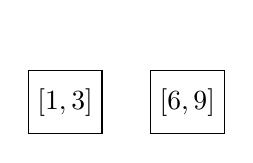
\begin{tikzpicture}
\node(0) {};
\node(1)[draw, rectangle, minimum size=8mm, below = 3mm of 0] {$[1,3]$};
\node(2)[draw, rectangle, minimum size=8mm, right= 6mm of 1.east, anchor=west] {$[6, 9]$};
\end{tikzpicture}
\par
\textbf{Output}:
\par
$[[1,5],[6,9]]$
\end{flushleft}
\paragraph{Example 2:}
\begin{flushleft}
\textbf{Input}:
\par
$I= [[1,2],[3,5],[6,7],[8,10],[12,16]]$, $\mu= [4,8]$
\par
\textbf{Output}: $[[1,2],[3,10],[12,16]]$
\par
\textbf{Explanation}:
\par
Because the new interval $[4,8]$ overlaps with $[3,5],[6,7],[8,10]$.
\end{flushleft} 

\subsection{Binary Search}
由于题目给出的interval都是按照起始位置按大小排序的,因为这些inteval都是不overlapp的,所以这些interval的end也是顺序排序的。所以自然而然就会用binary search。Denote $I$ 的长度为 $N$。
\par
首先找到一个interval $I[s]$,其起点$\alpha$是第一个大于或者等于$\mu$的起点 $\mu_{\alpha}$,即$I[s]_{\alpha} \geq \mu_{\alpha}$。如果$s=0$,意味着$I$中所有的interval的起点都不小于$\mu_{\alpha}$,很显然merge之后的interval的起点$\alpha$也就是$\mu_{\alpha}$。如果$s\neq 0$,那么我们需要比较$\mu_{\alpha}$与$I[s-1]$的end也就是$I[s-1]_{\beta}$。
\begin{itemize}
    \item If $\mu_{\alpha} \leq I[s-1]_{\beta}$,那么$I[s-1]$可以被merge,merge之后的interval的起始点$\alpha = I[s-1]_{\alpha}$。这种情况可以从下面的示图分析得出
    \begin{figure}[H]
        \centering
            \begin{tikzpicture}
            \node(0) {};
            \node (1) at (5, 0)  [draw, minimum width=4cm, minimum height=0.7cm, label = $\mu$, label=right:$\beta$, label=left:$\alpha$, anchor = south west] {};
            \node(2) at (3, 1.3cm) [draw, minimum width=3cm, minimum height=0.7cm, label = $I(s-1)$,label=right:$\beta$, label=left:$\alpha$, anchor = south west] {};
            \node(3) at (8, 1.3cm) [draw, minimum width=3cm, minimum height=0.7cm, label = $I(s)$, label=right:$\beta$, label=left:$\alpha$, anchor = south west] {};
            \end{tikzpicture}
        \caption{Previous Interval $I[s-1]$ is overlapped with $\mu$}
    \end{figure}
    \item If $\mu_{\alpha} > I[s-1]_{\beta}$,那么$I[s-1]$,merge之后的interval的起始点$\alpha$仍然是 $\mu_{\alpha}$。
        \begin{figure}[H]
        \centering
            \begin{tikzpicture}
            \node(0) {};
            \node (1) at (5, 0)  [draw, minimum width=4cm, minimum height=0.7cm, label = $\mu$, label=right:$\beta$, label=left:$\alpha$, anchor = south west] {};
            \node(2) at (1, 1.3cm) [draw, minimum width=3cm, minimum height=0.7cm, label = $I(s-1)$,label=right:$\beta$, label=left:$\alpha$, anchor = south west] {};
            \node(3) at (8, 1.3cm) [draw, minimum width=3cm, minimum height=0.7cm, label = $I(s)$, label=right:$\beta$, label=left:$\alpha$, anchor = south west] {};
            \end{tikzpicture}
        \caption{Previous Interval $I[s-1]$ Is Not Overlap With $\mu$}
    \end{figure}
\end{itemize}
接下来寻找$I[e]$,其end $I[e]_{\beta}$是第一个大于或者等于$\mu$的end $\mu_{\beta}$。如果$e = N$,就是说$I$中所有的interval的end都不大于$\mu_{\beta}$,显然merge之后interval的end就是$\mu_{\beta}$。如果$e < N$,则需要比较$I[e]$的起点即$I[e]_{\alpha}$与$\mu_{\beta}$的关系。
\begin{itemize}
    \item If $I[e]_{\alpha} \leq \mu_{\beta}$,那么$I[e]$就要被merge,merge之后的end 即为$I[e]_{\beta}$。
           \begin{figure}[H]
        \centering
            \begin{tikzpicture}
            \node(0) {};
            \node (1) at (3, 0)  [draw, minimum width=4cm, minimum height=0.7cm, label = $\mu$, label=right:$\beta$, label=left:$\alpha$, anchor = south west] {};
            \node(3) at (6, 1.3cm) [draw, minimum width=3cm, minimum height=0.7cm, label = $I(e)$, label=right:$\beta$, label=left:$\alpha$, anchor = south west] {};
            \end{tikzpicture}
        \caption{The Interval $I[e]$ Is Overlap With $\mu$}
    \end{figure}
    \item If $I[e]_{\alpha} > \mu_{\beta}$,两个interval没有overlap,$I[e]$不会被merge,这时merge之后的interval的end即为$\mu_{\beta}$
        \begin{figure}[H]
        \centering
            \begin{tikzpicture}
            \node(0) {};
            \node (1) at (3, 0)  [draw, minimum width=4cm, minimum height=0.7cm, label = $\mu$, label=right:$\beta$, label=left:$\alpha$, anchor = south west] {};
            \node(3) at (8, 1.3cm) [draw, minimum width=3cm, minimum height=0.7cm, label = $I(e)$, label=right:$\beta$, label=left:$\alpha$, anchor = south west] {};
            \end{tikzpicture}
        \caption{The Interval $I[e]$ Is Not Overlap With $\mu$}
    \end{figure}
\end{itemize}
这样$I[s\ldots e]$就是要被merge的intervals,不过有几个边界情况需要考虑:
\begin{itemize}
    \item $s = N$,这意味着新的interval $\mu$位于$I$中最后一个interval的右边,所以最后的结果就是将$\mu$放在$I$的末尾,i.e. $I \gets I + \mu$。
    \item $e = 0$,这表示$\mu$位于$I$中第一个interval的左边,所以最后的结果就是将$\mu$插入到$I$的第一个位置,i.e. $I \gets \mu + I$
    \item $s = e$,这表示$\mu$没有和$I$中任何一个interval overlap,但是由于$I[s-1]$位于$\mu$的左侧,$I[s]$肯定不会在$\mu$的左侧,所以需要把$\mu$插入到$I[s-1]$和$I[s]$中间,i.e. $I \gets I[0\ldots s-1] + \mu + I[s\ldots N-1]$
\end{itemize}

\setcounter{lstlisting}{0}
\begin{lstlisting}[style=customc, caption={Binary Search}]
vector<vector<int>> insert( vector<vector<int>>& intervals, vector<int>& newInterval )
{

    //find the first interval whose start is no less than newInterval's start

    int L = static_cast<int>( intervals.size() );

    int s = bs( intervals, newInterval[0], 0 );

    int merge_l = newInterval[0];

    if( s > 0 )
    {
        //compare end of intervals[s-1]
        //against start of newInterval
        if( intervals[s - 1][1] >= newInterval[0] )
        {
            //newInterval will cover intervals[s-1]
            //update the merged interval's left boundary
            merge_l = intervals[s - 1][0];

            s = s - 1; //the start index of intervals to be merged
        }
    }

    int merge_r = newInterval[1];

    //find the first interval whose end is no less than newInterval's end
    int e = bs( intervals, newInterval[1], 1 );

    if( e < L )
    {
        //compare start of intervals[e]
        //against end of newInterval
        if( intervals[e][0] <= newInterval[1] )
        {
            //intervals[e] can be merged with newInterval
            //update the merged interval's right boundary
            merge_r = intervals[e][1];
            e = e + 1;
        }
    }


    vector<vector<int>> ans;

    //remove intervals in range [s...e]
    for( int i = 0; i < s; ++i )
    {
        ans.emplace_back( intervals[i].begin(), intervals[i].end() );
    }

    ans.push_back( vector<int> {merge_l, merge_r} );

    for( int i = e; i < L; ++i )
    {
        ans.emplace_back( intervals[i].begin(), intervals[i].end() );
    }

    return ans;
}

//leftmost binary search
int bs( vector<vector<int>>& A, int T, int index )
{
    int l = 0;

    int r = static_cast<int>( A.size() );


    while( l < r )
    {
        int mid = ( l + r ) / 2;

        if( A[mid][index] < T )
        {
            l = mid + 1;
        }
        else
        {
            r = mid;
        }
    }

    return l;
}
\end{lstlisting}
%\section{58 --- Length of Last Word}
Given a string s consists of upper/lower-case alphabets and empty space characters `\textvisiblespace', return the length of last word in the string.
\par
If the last word does not exist, return 0.
\par
\textbf{Note}: A word is defined as a character sequence consists of non-space characters only.
\paragraph{Example:}
\begin{flushleft}
\textbf{Input}: \texttt{Hello World}
\par
\textbf{Output}: 5
\end{flushleft}
Easy question, starting from the end of the string to find.
%\section{59 --- Spiral Matrix II}
Given a positive integer $n$, generate a square matrix filled with elements from 1 to $n^2$ in spiral order.
\paragraph{Example:}
\begin{flushleft}
\textbf{Input}: 3
\par
\textbf{Output}:
\begin{figure}[H]
    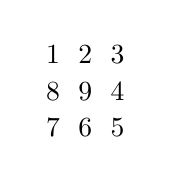
\begin{tikzpicture}
    \matrix (m) [matrix of nodes]
    {
        1 & 2 & 3 \\
        8 & 9 & 4 \\
        7 & 6 & 5 \\
    };
    \end{tikzpicture}
\end{figure}
\end{flushleft}
\subsection{Simulation}
和54题一模一样的方法,同样通过利用访问数组,不过因为这道题本身就是填充数组,所以我们可以用当前$M[r][c]$是否被填充了数来确定该元素是否已经访问过。避免了使用额外的访问数组。同时方向的安排需要按照spiral的顺序来定义,即$(0,1)\to(1,0)\to(0,-1)\to(-1,0)$
%\section{60 --- Permutation Sequence}
The set $[1,2,3,...,n]$ contains a total of $n!$ unique permutations.
\par
By listing and labeling all of the permutations in order, we get the following sequence for $n = 3$:
\[
123, 132, 213, 231, 312, 321
\]
\par
Given $n$ and $k$, return the $k$th permutation sequence.
\par
\textbf{Note}:
\par
Given $n$ will be between 1 and 9 inclusive.
\par
Given $k$ will be between 1 and n! inclusive.
\paragraph{Example 1:}
\begin{flushleft}
\textbf{Input}: $n = 3, k = 3$
\par
\textbf{Output}: $213$
\end{flushleft}
\paragraph{Example 2:}
\begin{flushleft}
\textbf{Input}: $n = 4, k = 9$
\par
\textbf{Output}: $2314$
\end{flushleft}
\subsection{Find the N-th permutation (Using factorial number system)} 
In this section, we are talking about the background of how to find $n$th permutation of a string. 
\subsection{Factorial Number System}
Instead of finding all permutations and looking up the $n$th, we can directly calculate the $n$th permutation. We need to first understand the \textbf{Factorial Number System.} A factorial number system uses \textbf{factorial} values instead of powers of numbers (binary system uses powers of 2, decimal uses powers of 10) to denote place-values (or base). The place values (base) are:
\[
0!=1, 1!=1, 2!=2, 3!=6, 4!=24, 5!=120, \ldots
\]
The digit in the zeroth place is always 0. The digit in the 1st place (with base = 1!) can be 0 or 1. The digit in the 2nd place (with base 2!) can be 0, 1 or 2 and so on. Generally speaking, the digit at $n$th place can take any value between $0\to n$.
\par
First few numbers represented as factoradics
\begin{align*}
    0 & \implies 0 = 0\times 0! \\
    1 & \implies 10 = 1*1! + 0*0! \\
    2 & \implies 100 = 1*2! + 0*1! + 0*0! \\
    3 & \implies 110 = 1\times 2! + 1\times 1! + 0\times 0! \\
    4 & \implies 200 = 2\times 2! + 0\times 1! + 0\times 0! \\
    5 & \implies 210 = 2\times 2! + 1\times 1! + 0\times 0! \\
    6 & \implies 1000 = 1\times 3! + 0\times 2! + 0\times 1! + 0\times 0! \\
    7 & \implies 1010 = 1\times 3! + 0\times 2! + 1\times 1! + 0\times 0! \\
    8 & \implies 1100 = 1\times 3! + 1\times 2! + 0\times 1! + 0\times 0! \\
    9 & \implies 1110 \\
    10& \implies 1200
\end{align*}
\par
There is a direct relationship between $n$th lexicographical permutation of a string and its factoradic representation.
\par
For example, here are the permutations of the string \textit{abcd}.
\begin{figure} [H]
    \centering
    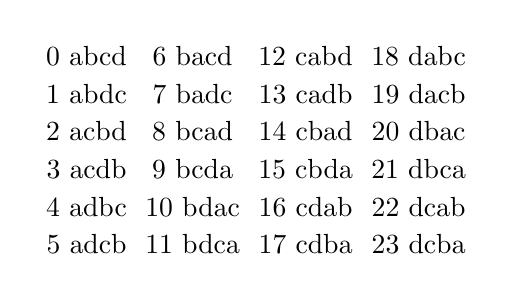
\begin{tikzpicture}
    \matrix (p) [matrix of nodes]
    {
    0  abcd & 6  bacd &  12  cabd & 18  dabc \\
    1  abdc & 7  badc &  13  cadb & 19  dacb \\
    2  acbd & 8  bcad &  14  cbad & 20  dbac \\
    3  acdb & 9  bcda &  15  cbda & 21  dbca \\
    4  adbc & 10  bdac & 16  cdab & 22  dcab \\
    5  adcb & 11  bdca & 17  cdba & 23  dcba \\
    };    
    \end{tikzpicture}
\end{figure}
\par
We can see a pattern here, if observed carefully. The first letter changes after every 6th ($3!$) permutation. The second letter changes after 2($2!$) permutation. The third letter changed after every ($1!$) permutation and the fourth letter changes after every ($0!$) permutation. We can use this relation to directly find the nth permutation.
\subsection{Algorithm}
Once we represent $n$ in factoradic representation, we consider each digit in it and add a character from the given string to the output. If we need to find the 14th permutation of \textbf{ABCD}. 14 in \textbf{factoradics} is 2100.
\begin{itemize}
    \item Start with the first digit \textbf{2}. Take the element at position 2 from \textbf{ABCD} which is \textbf{C}, and add it to the Output. Therefore, the output now is \textbf{C} and The previous string becomes \textbf{ABD}
    \item The next digit is \textbf{1}.String is now \textbf{ABCD}. Again, get the character at position 1 which is \textbf{B} and add it to the Output. Now, the output is \textbf{CB} and the previous string is \textbf{AD}
    \item Next digit is \textbf{0}. String is \textbf{AD}. Add the character at position 0 to the Output, we get output \textbf{CBA}. The previous string reduces to \textbf{D}
    \item Next digit is \textbf{0}. String is \textbf{D}. Add the character at position 0 to the Output, we get output \textbf{CBAD} and we consumed all characters from previous string.
\end{itemize}
In summary, we get the following process
\begin{figure}[H]
\centering
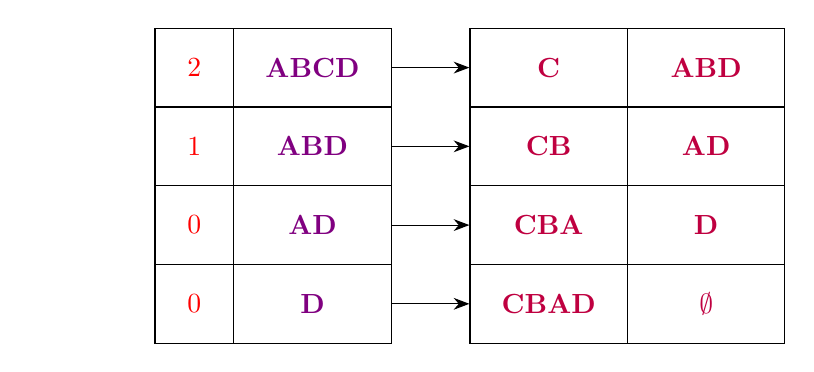
\begin{tikzpicture}
\node(0) {};
\node(2) at (2,0) [text=red, draw, minimum width=1cm, minimum height=1cm] {2};
\node(a) at (3.5,0) [text=violet, draw, minimum width=2cm, minimum height=1cm] {\textbf{ABCD}};
\node(c) at (6.5,0) [text=purple, draw, minimum width=2cm, minimum height=1cm] {\textbf{C}};
\node(d) at (8.5,0) [text=purple, draw, minimum width=2cm, minimum height=1cm] {\textbf{ABD}};
\draw[-{Stealth[length=2mm]}] (a) -- (c);
\node(1) at (2,-1) [text=red, draw, minimum width=1cm, minimum height=1cm] {1};
\node(a1) at (3.5,-1) [text=violet, draw, minimum width=2cm, minimum height=1cm] {\textbf{ABD}};
\node(c1) at (6.5,-1) [text=purple, draw, minimum width=2cm, minimum height=1cm] {\textbf{CB}};
\node(d1) at (8.5,-1) [text=purple, draw, minimum width=2cm, minimum height=1cm] {\textbf{AD}};
\draw[-{Stealth[length=2mm]}] (a1) -- (c1);
\node(0) at (2,-2) [text=red, draw, minimum width=1cm, minimum height=1cm] {0};
\node(a2) at (3.5,-2) [text=violet, draw, minimum width=2cm, minimum height=1cm] {\textbf{AD}};
\node(c2) at (6.5,-2) [text=purple, draw, minimum width=2cm, minimum height=1cm] {\textbf{CBA}};
\node(d2) at (8.5,-2) [text=purple, draw, minimum width=2cm, minimum height=1cm] {\textbf{D}};
\draw[-{Stealth[length=2mm]}] (a2) -- (c2);
\node at (2,-3) [text=red, draw, minimum width=1cm, minimum height=1cm] {0};
\node(a3) at (3.5,-3) [text=violet, draw, minimum width=2cm, minimum height=1cm] {\textbf{D}};
\node(c3) at (6.5,-3) [text=purple, draw, minimum width=2cm, minimum height=1cm] {\textbf{CBAD}};
\node at (8.5,-3) [text=purple, draw, minimum width=2cm, minimum height=1cm] {$\emptyset$};
\draw[-{Stealth[length=2mm]}] (a3) -- (c3);
\end{tikzpicture}
\end{figure}
\subsection{Convert To Factorial Number}
To convert a given number to Factorial Number System,successively divide the number by $1,2,3,4,5,6$ and so on until the quotient becomes zero. The reminders at each step forms the factoradic representation.
\par
For example, to convert $349$ to factoradic, we have the following process
\begin{itemize}
    \item $\dfrac{349}{1} = 349$, we have remainders $r = 0$ and quotient $q = 349$, the generated factoradic number $\digamma = 0$
    \item $\dfrac{349}{2} = 174$, $r = 1, q = 174,\; \digamma = 10$
    \item $\dfrac{174}{3} = 58$, $r = 0, q = 58,\; \digamma = 010$
    \item $\dfrac{58}{4} = 14$, $r = 2, q = 14,\; \digamma = 2010$
    \item $\dfrac{14}{5} = 2$, $r = 4, q = 2,\; \digamma = 42010$
    \item $\dfrac{2}{6} = 0$, $r = 2, q = 0,\; \digamma = 242010$
\end{itemize}
Hence, Factoradic representation of 349 is \textbf{242010}. \textbf{Note}: The length of factoradic representation should be equal to the length of the character array. Prepend zeros to ensure the length is same.

\setcounter{lstlisting}{0}
\begin{lstlisting}[style=customc, caption={Factorial Number System}]
string getPermutation( int n, int k )
{
    vector<int> factors( n, 0 );

    int factor = 1;

    //k is in [0, n!-1]
    --k;

    //fill the coefficients of factorial number
    while( k )
    {
        int q = k / factor;
        int r = k - q * factor;

        factors[factor - 1] = r;

        k = q;
        ++factor;
    }

    string s;
    for( int i = 1; i <= n; ++i )
    {
        s.push_back( i + '0' );
    }

    string ans;

    //generate the k-th permutation
    //based on factors array
    for( size_t i = 0; i < factors.size(); ++i )
    {

        auto j = factors.size() - i - 1;

        int sel = factors[j];
        ans.push_back( s[sel] );

        s = s.substr( 0, sel ) + s.substr( sel + 1 );
    }

    return ans;
}
\end{lstlisting}
\section{61 --- Rotate List}
Given a linked list $\eta_0$, rotate the list to the right by $k$ places, where $k$ is non-negative.
\paragraph{Example 1:}
\begin{flushleft}
\textbf{Input:}
\\
\begin{figure}[H]
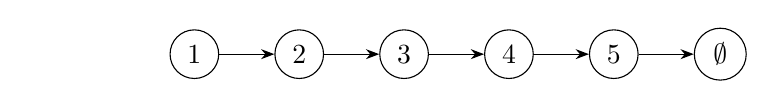
\begin{tikzpicture}
\node{};
\node(1) at (2,0)[draw, circle] {1};
\node(2) [draw, circle, right = 0.7cm of 1] {2};
\node(3) [draw, circle, right = 0.7cm of 2] {3};
\node(4) [draw, circle, right = 0.7cm of 3] {4};
\node(5) [draw, circle, right = 0.7cm of 4] {5};
\node(6) [draw, circle, right = 0.7cm of 5] {$\emptyset$};
\draw[-{Stealth}] (1) -- (2);
\draw[-{Stealth}] (2) -- (3);
\draw[-{Stealth}] (3) -- (4);
\draw[-{Stealth}] (4) -- (5);
\draw[-{Stealth}] (5) -- (6);
\end{tikzpicture}
\end{figure}
$k=2$
\\
\textbf{Output:}
\\
\begin{figure}[H]
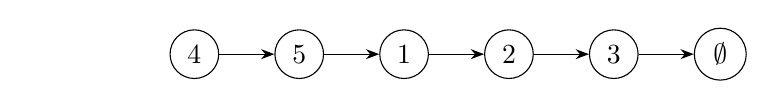
\begin{tikzpicture}
\node{};
\node(1) at (2,0)[draw, circle] {4};
\node(2) [draw, circle, right = 0.7cm of 1] {5};
\node(3) [draw, circle, right = 0.7cm of 2] {1};
\node(4) [draw, circle, right = 0.7cm of 3] {2};
\node(5) [draw, circle, right = 0.7cm of 4] {3};
\node(6) [draw, circle, right = 0.7cm of 5] {$\emptyset$};
\draw[-{Stealth}] (1) -- (2);
\draw[-{Stealth}] (2) -- (3);
\draw[-{Stealth}] (3) -- (4);
\draw[-{Stealth}] (4) -- (5);
\draw[-{Stealth}] (5) -- (6);
\end{tikzpicture}
\end{figure}
\textbf{Explanation}:
\par
rotate 1 steps to the right:
\\
\begin{figure}[H]
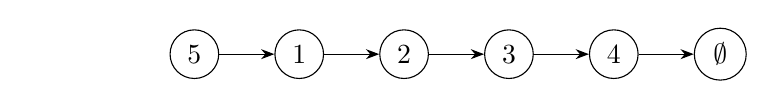
\begin{tikzpicture}
\node{};
\node(1) at (2,0)[draw, circle] {5};
\node(2) [draw, circle, right = 0.7cm of 1] {1};
\node(3) [draw, circle, right = 0.7cm of 2] {2};
\node(4) [draw, circle, right = 0.7cm of 3] {3};
\node(5) [draw, circle, right = 0.7cm of 4] {4};
\node(6) [draw, circle, right = 0.7cm of 5] {$\emptyset$};
\draw[-{Stealth}] (1) -- (2);
\draw[-{Stealth}] (2) -- (3);
\draw[-{Stealth}] (3) -- (4);
\draw[-{Stealth}] (4) -- (5);
\draw[-{Stealth}] (5) -- (6);
\end{tikzpicture}
\end{figure}
rotate 2 steps to the right:
\\
\begin{figure}[H]
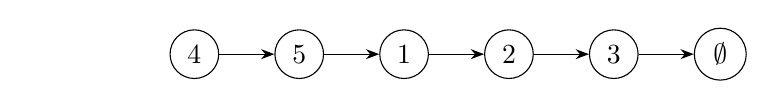
\begin{tikzpicture}
\node{};
\node(1) at (2,0)[draw, circle] {4};
\node(2) [draw, circle, right = 0.7cm of 1] {5};
\node(3) [draw, circle, right = 0.7cm of 2] {1};
\node(4) [draw, circle, right = 0.7cm of 3] {2};
\node(5) [draw, circle, right = 0.7cm of 4] {3};
\node(6) [draw, circle, right = 0.7cm of 5] {$\emptyset$};
\draw[-{Stealth}] (1) -- (2);
\draw[-{Stealth}] (2) -- (3);
\draw[-{Stealth}] (3) -- (4);
\draw[-{Stealth}] (4) -- (5);
\draw[-{Stealth}] (5) -- (6);
\end{tikzpicture}
\end{figure}
\end{flushleft}
\paragraph{Example 2:}
\begin{flushleft}
\textbf{Input}:
\\
\begin{figure}[H]
\begin{tikzpicture}
\node{};
\node(1) at (2,0)[draw, circle] {0};
\node(2) [draw, circle, right = 0.7cm of 1] {1};
\node(3) [draw, circle, right = 0.7cm of 2] {2};
\node(4) [draw, circle, right = 0.7cm of 3] {$\emptyset$};
\draw[-{Stealth}] (1) -- (2);
\draw[-{Stealth}] (2) -- (3);
\draw[-{Stealth}] (3) -- (4);
\end{tikzpicture}
\end{figure}
$k = 4$
\\
\textbf{Output:}
\\
\begin{figure}[H]
\begin{tikzpicture}
\node{};
\node(1) at (2,0)[draw, circle] {2};
\node(2) [draw, circle, right = 0.7cm of 1] {0};
\node(3) [draw, circle, right = 0.7cm of 2] {1};
\node(4) [draw, circle, right = 0.7cm of 3] {$\emptyset$};
\draw[-{Stealth}] (1) -- (2);
\draw[-{Stealth}] (2) -- (3);
\draw[-{Stealth}] (3) -- (4);
\end{tikzpicture}
\end{figure}
\textbf{Explanation}:
\\
rotate 1 steps to the right:
\\
\begin{figure}[H]
\begin{tikzpicture}
\node{};
\node(1) at (2,0)[draw, circle] {2};
\node(2) [draw, circle, right = 0.7cm of 1] {0};
\node(3) [draw, circle, right = 0.7cm of 2] {1};
\node(4) [draw, circle, right = 0.7cm of 3] {$\emptyset$};
\draw[-{Stealth}] (1) -- (2);
\draw[-{Stealth}] (2) -- (3);
\draw[-{Stealth}] (3) -- (4);
\end{tikzpicture}
\end{figure}
rotate 2 steps to the right: 
\\
\begin{figure}[H]
\begin{tikzpicture}
\node{};
\node(1) at (2,0)[draw, circle] {1};
\node(2) [draw, circle, right = 0.7cm of 1] {2};
\node(3) [draw, circle, right = 0.7cm of 2] {0};
\node(4) [draw, circle, right = 0.7cm of 3] {$\emptyset$};
\draw[-{Stealth}] (1) -- (2);
\draw[-{Stealth}] (2) -- (3);
\draw[-{Stealth}] (3) -- (4);
\end{tikzpicture}
\end{figure}
rotate 3 steps to the right:
\\
\begin{figure}[H]
\begin{tikzpicture}
\node{};
\node(1) at (2,0)[draw, circle] {0};
\node(2) [draw, circle, right = 0.7cm of 1] {1};
\node(3) [draw, circle, right = 0.7cm of 2] {2};
\node(4) [draw, circle, right = 0.7cm of 3] {$\emptyset$};
\draw[-{Stealth}] (1) -- (2);
\draw[-{Stealth}] (2) -- (3);
\draw[-{Stealth}] (3) -- (4);
\end{tikzpicture}
\end{figure}
rotate 4 steps to the right:
\\
\begin{figure}[H]
\begin{tikzpicture}
\node{};
\node(1) at (2,0)[draw, circle] {2};
\node(2) [draw, circle, right = 0.7cm of 1] {0};
\node(3) [draw, circle, right = 0.7cm of 2] {1};
\node(4) [draw, circle, right = 0.7cm of 3] {$\emptyset$};
\draw[-{Stealth}] (1) -- (2);
\draw[-{Stealth}] (2) -- (3);
\draw[-{Stealth}] (3) -- (4);
\end{tikzpicture}
\end{figure}
\end{flushleft}

\subsection{Analysis}
The nodes in the list are already linked, and hence the rotation basically means

\begin{itemize}
\item To close the linked list into the ring.
\item To break the ring after the new tail and just in front of the new head
\end{itemize}

Suppose $k=2$ and the list is shown as below:

\begin{figure}[H]
\begin{tikzpicture}
[start chain, 
every node/.style={draw, circle,
 minimum size=6mm, fill=gray!20!, on chain},
  node distance=8mm, 
  every join/.style={>=stealth,->},
  every on chain/.style={join=by ->},
 thick
]
\node{1};
\node{2};
\node{3};
\node{4};
\node{5};
\node{};
\end{tikzpicture}
\end{figure}

The steps to rotate the list by $k=2$ places are shown as below:

\begin{enumerate}
\item Link the head and the tail
\begin{figure}[H]
\begin{tikzpicture}
[start chain, 
every node/.style={draw, circle,
 minimum size=6mm, fill=gray!20!, on chain},
  node distance=8mm, 
  every join/.style={>=stealth,->},
  every on chain/.style={join=by ->},
 thick
]
\node(1){1};
\node(2){2};
\node(3){3};
\node(4){4};
\node(5){5};
\draw[very thick, red, >=stealth, ->] (5.south) -- ++(0, -10mm) -| (1.south);
\end{tikzpicture}
\end{figure}
\item Break 3 and 4, and set node 3 as the final non-empty node.
\begin{figure}[H]
\begin{tikzpicture}
[every node/.style={draw, circle,
 minimum size=6mm, fill=gray!20!, on chain},
  node distance=8mm, 
  every join/.style={>=stealth,->},
 thick
]
\node(1){1};
\node(2)[join]{2};
\node(3)[join]{3};
\node[join]{};
\node(4){4};
\node(5)[join]{5};
\draw[very thick, red, >=stealth, ->] (5.south) -- ++(0, -10mm) -| (1.south);
\end{tikzpicture}
\end{figure}
\item The new head is in the position $n-k$, where $n$ is a number of nodes in the list. The new tail is just before the new head, which is in the position $n - k - 1$.
\item When $k\geq n$, just use $k\bmod n$ to change $k$ to less than $n$.
\end{enumerate}

Thus, the algorithm is quite straightforward :

\begin{itemize}
\item Find the old tail and connect it with the head to form a close ring. Compute the length of the list n at the same time.

\item Find the new tail, which is $(n - (k\bmod n) - 1)$th node from the head, and the new head, which is $(n - (k\bmod n))$th node.

\item Break the ring by set the new tail's next node as empty node, and the new head.
\end{itemize}

\setcounter{lstlisting}{0}
\begin{lstlisting}[style=customc, caption={Direct Way}]
ListNode* rotateRight( ListNode* head, int k )
{
    if( !head )
    {
        return head;
    }

    auto node = head;

    int n = 1;

    while( node->next )
    {
        ++n;
        node = node->next;
    }

    //close the ring
    node->next = head;

    //the new tail's position
    auto new_tail = head;

    int pos = n - ( k % n ) - 1;
    for( int i = 0; i < pos; ++i )
    {
        new_tail = new_tail->next;
    }

    auto new_head = new_tail->next;
    new_tail->next = nullptr;

    return new_head;
}
\end{lstlisting}
\section{62 --- Unique Paths}
A robot is located at the top-left corner of a $m \times n$ grid.
\par
The robot can only move either down or right at any point in time. The robot is trying to reach the bottom-right corner of the grid.
\begin{figure}[H]
\begin{tikzpicture}
\draw[step=1.5cm, help lines, thick] (0,0) grid ++(10.5,4.5);
\node[bob, minimum size=1cm] at (0.75, 3.75) {};
\node[star, fill=green!40, star points = 5, draw, star point height=0.2cm, minimum size=1cm] at(9.75, 0.75) {};
\end{tikzpicture}
\end{figure}
How many possible unique paths are there?
\\
\paragraph{Note:}
\begin{itemize}
\item $m$ and $n$ will be at most 100.
\end{itemize}
\paragraph{Example 1:}
\begin{flushleft}
\textbf{Input}: $m = 3, n = 2$
\\
\textbf{Output}: 3
\\
\textbf{Explanation}:
\\
From the top-left corner, there are a total of 3 ways to reach the bottom-right corner:
\begin{enumerate}
\item Right $\to$ Right $\to$ Down
\item Right $\to$ Down $\to$ Right
\item Down $\to$ Right $\to$ Right
\end{enumerate}
\end{flushleft}

\paragraph{Example 2:}
\begin{flushleft}
\textbf{Input}: $m = 7, n = 3$
\\
\textbf{Output}: 28
\end{flushleft}

\subsection{Dynamic Programming}
Suppose $F[i][j]$ is the number of unique paths from $(0,0)$ to $(i,j)$. 

由于robot只能向右或者向下走,所以,move 到 $(i,j)$ 必须首先 move 到 $(i-1, j)$ 或者 $(i, j-1)$,因此 recursive function $F[i][j] = F[i-1][j] + F[i][j-1]$。对于第一行或者第一列的每个位置,很显然到这些位置的unique path 只有一个。

\setcounter{lstlisting}{0}
\begin{lstlisting}[style=customc, caption={Two Dimensional DP}]
int uniquePaths( int m, int n )
{
    vector<vector<int>> F( m, vector<int>( n, 0 ) );

    F[0][0] = 1;

    //since the only move direction is down or right
    //the first row and column will be 1
    for( int i = 1; i < m; ++i )
    {
        F[i][0] = 1;
    }

    for( int j = 1; j < n; ++j )
    {
        F[0][j] = 1;
    }

    for( int i = 1; i < m; ++i )
    {
        for( int j = 1; j < n; ++j )
        {
            F[i][j] = F[i - 1][j] + F[i][j - 1];
        }
    }

    return F[m - 1][n - 1];

}
\end{lstlisting}

Notice that each time when we update $F[i][j]$, we only need $F[i - 1][j]$ (at the previous row) and $F[i][j - 1]$ (at the current row). So we can reduce the memory usage to just two rows.

\begin{lstlisting}[style=customc, caption={Two One Dimension DP Array}]
int uniquePaths( int m, int n )
{
    vector<int> pre_row( n, 1 );
    vector<int> cur_row( n, 1 );

    for( int i = 1; i < m; ++i )
    {
        for( int j = 1; j < n; ++j )
        {
            cur_row[j] = pre_row[j] + cur_row[j - 1];
        }

        swap( cur_row, pre_row );
    }

    //last time, cur_row is swapped to pre_row
    //therefore, the answer is in pre_row
    return pre_row[n - 1];
}
\end{lstlisting}

We can see only one dimension array is required 

\begin{lstlisting}[style=customc, caption={One Dimension DP Array}]
int uniquePaths( int m, int n )
{
    vector<int> cur_row( n, 1 );

    for( int i = 1; i < m; ++i )
    {
        for( int j = 1; j < n; ++j )
        {
            //update current row directly
            cur_row[j] += cur_row[j - 1];
        }
    }

    return cur_row[n - 1];
}
\end{lstlisting}
\section{63 --- Unique Paths II}
A robot is located at the top-left corner of a $m \times n$ grid (marked \textbf{Start} in the diagram below).
\par
The robot can only move either down or right at any point in time. The robot is trying to reach the bottom-right corner of the grid (marked \textbf{Finish} in the diagram below)
\par
Now consider if some obstacles are added to the grids. How many unique paths would there be?
\par
An obstacle and empty space is marked as 1 and 0 respectively in the grid.

\paragraph{Note:}
\begin{itemize}
\item $m$ and $n$ will be at most 100.
\end{itemize}

\subsection{Dynamic Programming}
Same as Problem 62. The only difference is that for the obstacle, $F[i][j]=0$

\paragraph{Example 1:}
\begin{flushleft}
\textbf{Input}:
\begin{figure}[H]
\begin{tikzpicture}
\matrix [matrix of nodes]
{
	0 & 0 & 0 \\
	0 & 1 & 0 \\
	0 & 0 & 0 \\
};
\end{tikzpicture}
\end{figure}
\textbf{Output}: 2
\\
\textbf{Explanation}:
\\
There is one obstacle in the middle of the $3\times 3$ grid above.
There are two ways to reach the bottom-right corner
\begin{enumerate}
\item Right$\to$Right$\to$Down$\to$Down
\item Down$\to$Down$\to$Right$\to$Right
\end{enumerate}
\end{flushleft}
%\section{64 --- Minimum Path Sum}
Given a $m \times n$ grid filled with non-negative numbers, find a path from top left to bottom right which minimizes the sum of all numbers along its path.

Note: You can only move either down or right at any point in time.

\paragraph{Example:}
\begin{flushleft}


\textbf{Input}:
\[
\begin{bmatrix}
1 & 3 & 1\\
1 & 5 & 1\\
4 & 2 & 1
\end{bmatrix}
\]

\textbf{Output}: 7

\textbf{Explanation}: Because the path $1\to 3 \to 1 \to 1 \to 1$ minimizes the sum.


\end{flushleft}

\subsection{Dynamic Programming 2D}
Suppose $F[i][j]$ is the minimum sum of the path from the index $(i,j)$ to the bottom rightmost element. 

We start by initializing the bottom rightmost element of $F$ as the last element of the given matrix. Then for each element starting from the bottom right, we traverse backwards and fill in the matrix with the required minimum sums. 

Now, we need to note that at every element, we can move either rightwards or downwards. Therefore, for filling in the minimum sum, we use the equation: $F[i][j] = G[i][j] + \min(F[i+1][j], F[i][j+1])$.

\setcounter{lstlisting}{0}
\begin{lstlisting}[style=customc, caption={2D DP}]
int minPathSum( vector<vector<int>>& grid )
{
    auto M = grid.size();
    auto N = grid[0].size();

    vector<vector<int>> F( M, vector<int>( N, 0 ) );

    F[M - 1][N - 1] = grid[M - 1][N - 1];
    //fill the right column
    for( size_t r = M - 1; r >= 1; --r )
    {
        F[r - 1][N - 1] = F[r][N - 1] + grid[r - 1][N - 1];
    }
    //fill the last row
    for( size_t c = N - 1; c >= 1; --c )
    {
        F[M - 1][c - 1] = F[M - 1][c] + grid[M - 1][c - 1];
    }
    //Fill DP from bottom right to to left
    for( size_t r = M - 1; r >= 1; --r )
    {
        for( size_t c = N - 1; c >= 1; --c )
        {
            //current value plus minimum of
            //its right and down neighbors
            F[r - 1][c - 1] = grid[r - 1][c - 1] + ( min )( F[r][c - 1], F[r - 1][c] );
        }
    }

    return F[0][0];
}
\end{lstlisting}
%\section{65 --- Valid Number}
Validate if a given string can be interpreted as a decimal number.

\paragraph{Some examples:}

\begin{flushleft}


\fcc{"0" => true}

\fcc{" 0.1 " => true}

\fcc{"abc" => false}

\fcc{"1 a" => false}

\fcc{"2e10" => true}

\fcc{" -90e3   " => true}

\fcc{" 1e" => false}

\fcc{"e3" => false}

\fcc{" 6e-1" => true}

\fcc{" 99e2.5 " => false}

\fcc{"53.5e93" => true}

\fcc{" --6 " => false}

\fcc{"-+3" => false}

\fcc{"95a54e53" => false}

\end{flushleft}

\paragraph{Note:} 

It is intended for the problem statement to be ambiguous. You should gather all requirements up front before implementing one. However, here is a list of characters that can be in a valid decimal number:

\begin{itemize}
\item Numbers 0-9
\item Exponent - \fcc{"e"}
\item Positive/negative sign \fcc{- "+"/"-"}
\item Decimal point - \fcc{"."}
\end{itemize}
%\section{66 --- Plus One}
Given a non-empty array of digits representing a non-negative integer, plus one to the integer.

The digits are stored such that the most significant digit is at the head of the list, and each element in the array contain a single digit.

You may assume the integer does not contain any leading zero, except the number 0 itself.

\paragraph{Example 1:}

\begin{flushleft}
\textbf{Input}: \fcj{[1,2,3]}

\textbf{Output}: \fcj{[1,2,4]}

\textbf{Explanation}: The array represents the integer 123.
\end{flushleft}

\paragraph{Example 2:}

\begin{flushleft}
\textbf{Input}: \fcj{[4,3,2,1]}

\textbf{Output}: \fcj{[4,3,2,2]}

\textbf{Explanation}: The array represents the integer 4321.
\end{flushleft}
%\section{67 --- Add Binary}
Given two binary strings, return their sum (also a binary string).

The input strings are both \textbf{non-empty} and contains only characters 1 or 0.

\paragraph{Example 1:}

\begin{flushleft}
\textbf{Input}: \fcj{a = "11"}, \fcj{b = "1"}

\textbf{Output}: \fcj{"100"}
\end{flushleft}

\paragraph{Example 2:}

\begin{flushleft}
\textbf{Input}: \fcj{a = "1010"}, \fcj{b = "1011"}

\textbf{Output}: \fcj{"10101"}
\end{flushleft}
%\section{68 --- Text Justification}
Given an array of words and a width \fcj{maxWidth}, format the text such that each line has exactly \fcj{maxWidth} characters and is fully (left and right) justified.

You should pack your words in a greedy approach; that is, pack as many words as you can in each line. Pad extra spaces \fcj{' '} when necessary so that each line has exactly \fcj{maxWidth} characters.

Extra spaces between words should be distributed as evenly as possible. If the number of spaces on a line do not divide evenly between words, the empty slots on the left will be assigned more spaces than the slots on the right.

For the last line of text, it should be left justified and no extra space is inserted between words.

\paragraph{Note:}

\begin{itemize}
\item A word is defined as a character sequence consisting of non-space characters only.

\item Each word's length is guaranteed to be greater than 0 and not exceed \fcj{maxWidth}.

\item The input array \fcj{words} contains at least one word.

\end{itemize}

\paragraph{Example 1:}
\begin{flushleft}


\textbf{Input}:

\fcj{words = ["This", "is", "an", "example", "of", "text", "justification."]}

\fcj{maxWidth = 16}

\textbf{Output}:

\begin{lstlisting}[style=customc]
[
   "This    is    an",
   "example  of text",
   "justification.  "
]
\end{lstlisting}
\end{flushleft}

\paragraph{Example 2:}
\begin{flushleft}

\textbf{Input}:

\fcj{words = ["What","must","be","acknowledgment","shall","be"]}

\fcj{maxWidth = 16}

\textbf{Output}:
\begin{lstlisting}[style=customc]
[
  "What   must   be",
  "acknowledgment  ",
  "shall be        "
]
\end{lstlisting}

\textbf{Explanation}: 

Note that the last line is \fcj{"shall be    "} instead of \fcj{"shall     be"},

because the last line must be left-justified instead of fully-justified.

Note that the second line is also left-justified becase it contains only one word.

\end{flushleft}

\paragraph{Example 3:}
\begin{flushleft}


\textbf{Input}:
\begin{lstlisting}[style=customc]
words = ["Science","is","what","we","understand","well","enough","to",
"explain", "to","a","computer.",
"Art","is","everything","else","we","do"]
\end{lstlisting}

\fcj{maxWidth = 20}

\textbf{Output}:
\begin{lstlisting}[style=customc]
[
  "Science  is  what we",
  "understand      well",
  "enough to explain to",
  "a  computer.  Art is",
  "everything  else  we",
  "do                  "
]
\end{lstlisting}
\end{flushleft}

\subsection{Greedy}
The algorithm can be divided into three steps:
\begin{enumerate}
\item Check if current word can be added into current line
\item Determine how many spaces we need to insert
\item Process the last line.
\end{enumerate}

We make use of an array $T$ to record added words.

To check if current word can be added to $T$
\begin{itemize}
\item Get total characters $x$ By assuming insert only one space between words in $T$ and current word.
\item If $x < L$ ($L$ is \fcj{maxWidth}), we add current word into $T$. Otherwise, we pad all the words in $T$ with spaces.
\end{itemize}

To pad the words in $T$, 
\begin{enumerate}
\item Get total length of all words, say $\ell$, in $T$.
\item Get number of words in $T$, say $y$.
\item The average number of spaces, say, $z$, inserted between two consecutive words are $\ell/(y-1)$.
\item The extra spaces, say $r$, will be $\bmod(\ell, y-1)$.
\item To greedily used extra spaces, for the first $r+1$ words, the inserted spaces between two consecutive ones are $ z + 1$
\end{enumerate}

If there is only word in $T$, we just print the word and pad with required spaces.

\setcounter{lstlisting}{0}
\begin{lstlisting}[style=customc, caption={Greedy}]
vector<string> fullJustify( vector<string>& words, int maxWidth )
{
    size_t L = static_cast< size_t >( maxWidth );
    //record selected word in current line
    vector<string_view> text;
    //total length of selected word in current line
    size_t text_len = 0;

    vector<string> ans;

    for( const auto& word : words )
    {
        //assume we put only one space between already selected words
        //and this word, we may need <text.size() - 1 + 1 = text.size()> spaces
        auto spaces = text.size();
        //check if we can select <word>
        if( text_len + spaces + word.size() <= L )
        {
            //add <word> into current line <text>
            text.emplace_back( word.c_str(), word.size() );
            //update <text_len>
            text_len += word.size();
        }
        else
        {
            //we will arrange current line <text>
            string line = gen_line( text, text_len, L );
            ans.push_back( "" );
            ans.back().swap( line );

            //remove all current words in the <text>
            text.clear();
            //add current word
            text.emplace_back( word.c_str(), word.size() );
            //reset total length of selected words
            text_len = word.size();
        }
    }//end for(word)

    //add final line
    string line;
    line.reserve( L );

    //we add each word plus one space
    auto spaces = L - text_len;

    for( size_t i = 0; i < text.size() - 1; ++i )
    {
        line += text[i];
        line.append( 1, ' ' );
        --spaces;
    }
    //add last word
    line += text.back();
    if( spaces )
    {
        //pad spaces
        line.append( spaces, ' ' );
    }

    ans.emplace_back( line );
    return ans;
}
//helper function to generate left justified line
string gen_line( vector<string_view>& text, size_t text_len, size_t L )
{
    //the required spaces to be inserted
    auto spaces = L - text_len;

    string line;
    line.reserve( L );

    if( text.size() == 1 )
    {
        //we only have one word in this line
        //just add the word and required spaces
        line += text[0];
        line.append( spaces, ' ' );

        return line;
    }
    //the number of spaces between two words
    auto sep_spaces = spaces / ( text.size() - 1 );
    //the number of extra spaces will put in the front of line
    auto extra_spaces = spaces - sep_spaces * ( text.size() - 1 );

    for( size_t i = 0; i < text.size() - 1; ++i )
    {
        line += text[i];
        auto insert_spaces = sep_spaces;
        if( extra_spaces )
        {
            //we insert one more space
            //to consume extra spaces
            ++insert_spaces;
            --extra_spaces;
        }
        line.append( insert_spaces, ' ' );
    }

    //add final word
    line += text.back();

    return line;
}
\end{lstlisting}
%\section{69 --- Sqrt(x)}
Implement \fcc{int sqrt(int x)}.

Compute and return the square root of $x$, where $x$ is guaranteed to be a non-negative integer.

Since the return type is an integer, the decimal digits are truncated and only the integer part of the result is returned.

\paragraph{Example 1:}

\begin{flushleft}
\textbf{Input}: 4

\textbf{Output}: 2
\end{flushleft}

\paragraph{Example 2:}

\begin{flushleft}
\textbf{Input}: 8

\textbf{Output}: 2

\textbf{Explanation}: 

The square root of 8 is $2.82842\ldots$, and since the decimal part is truncated, 2 is returned.
\end{flushleft}

\subsection{Binary Search}
For $x \ge 2$, the square root is always smaller than $x / 2$ and larger than 0: $0 < a < x / 2$.

Since $a$ is an integer, the problem goes down to the iteration over the sorted set of integer numbers. Here the binary search enters the scene.

We can use a leftmost binary search to find the square root

\setcounter{lstlisting}{0}
\begin{lstlisting}[style=customc, caption={Binary Search}]
int mySqrt( int x )
{
    if( x < 2 )
    {
        return x;
    }
    //the square root
    //is in [2, x/2]
    int l = 2;
    int r = x / 2 + 1;
    //leftmost binary search
    while( l < r )
    {
        auto mid = static_cast<long long>( ( l + r ) / 2 );

        if( mid * mid < x )
        {
            l = mid + 1;
        }
        else
        {
            r = mid;
        }
    }
    //check if l*l=x
    auto y = static_cast<long long>( l );
    if( y * y == x )
    {
        return l;
    }
    //return the previous one
    return l - 1;
}
\end{lstlisting}
% \section{78 --- Subsets}
Given a set of distinct integers, $A$, return all possible subsets (the power set).
\par
Note: The solution set must not contain duplicate subsets.
\paragraph{Example:}
\begin{flushleft}
\textbf{Input}: $A = [1,2,3]$
\\
\textbf{Output}:
$(3), (1), (2), (1,2,3), (1,3),  (2,3),  (1,2), () $
\end{flushleft}
\subsection{Backtracking}
原来的set中每一个element在subset中有两种状态:要么存在、要么不存在。这样构造subset的过程中每个element有两种选择方法:选择、不选择,因此可以构造一颗二叉树,例如给出的例子$A=[1,2,3]$,构造的二叉树如下(左子树表示选择该层处理的元素,右子树不选择),最后得到的叶子节点就是子集:
\begin{figure}[H]
\begin{tikzpicture}
[mynode/.style={draw, minimum size=1cm, fill=gray!20!}]
\node(){};
\node[mynode](rt){};
\node[mynode](l1) [below = 8mm of rt, xshift=-3.8cm] {$(1)$};
\node[mynode](r1) [below = 8mm of rt, xshift=3.8cm] {};
\node[mynode](ll) [below = 8mm of l1, xshift=-2cm] {$(1,2)$};
\node[mynode](lr) [below = 8mm of l1, xshift=2cm] {$(1)$};
\node[mynode](rl) [below = 8mm of r1, xshift=-2cm] {$(2)$};
\node[mynode](rr) [below = 8mm of r1, xshift=2cm] {};
\node[mynode](lll) [below = 8mm of ll, xshift=-1cm] {$(1,2,3)$};
\node[mynode](llr) [below = 8mm of ll, xshift=1cm] {$(1,2)$};
\node[mynode](lrl) [below = 8mm of lr, xshift=-1cm] {$(1,3)$};
\node[mynode](lrr) [below = 8mm of lr, xshift=1cm] {$(1)$};
\node[mynode](rll) [below = 8mm of rl, xshift=-1cm] {$(2,3)$};
\node[mynode](rlr) [below = 8mm of rl, xshift=1cm] {$(2)$};
\node[mynode](rrl) [below = 8mm of rr, xshift=-1cm] {$(3)$};
\node[mynode](rrr) [below = 8mm of rr, xshift=1cm] {};
\draw[>=stealth,->] (rt) -- (l1.north east);
\draw[>=stealth,->] (rt) -- (r1.north west);
\draw[>=stealth,->] (l1) -- (ll);
\draw[>=stealth,->] (l1) -- (lr);
\draw[>=stealth,->] (ll) -- (lll);
\draw[>=stealth,->] (ll) -- (llr);
\draw[>=stealth,->] (lr) -- (lrl);
\draw[>=stealth,->] (lr) -- (lrr);
\draw[>=stealth,->] (r1) -- (rl);
\draw[>=stealth,->] (r1) -- (rr);
\draw[>=stealth,->] (rl) -- (rll);
\draw[>=stealth,->] (rl) -- (rlr);
\draw[>=stealth,->] (rr) -- (rrl);
\draw[>=stealth,->] (rr) -- (rrr);
\end{tikzpicture}
\end{figure}
根据上述二叉树,递归函数中需要从某个位置开始,向当前level的数组中加入该位置的数字,然后继续递归,结束后,把这个数字移除出数组。类似的题目都有类似这样的递归结构。原来的题目中还有个要求是subset中的数字必须是非递减序列,因此首先需要对数组进行排序。
\subsubsection{Code}
\setcounter{algorithm}{0}
\begin{algorithm}[H]
\caption{Depth First Search}
\begin{algorithmic}[1]
\Procedure{Subsets}{$A, L$}
\State $\texttt{sort}(A)$
\State $V:=\emptyset$ \Comment Empty array to hold current subset
\State $\texttt{ans}:=\emptyset$ \Comment The result subsets
\State $\texttt{DFS}(A, L, V, \texttt{ans}, 0)$ \Comment Call recursive function \texttt{DFS}
\State \Return \texttt{ans}
\EndProcedure
\end{algorithmic}
\end{algorithm}

\begin{algorithm}[H]
\caption{Recursive Function}
\begin{algorithmic}[1]
\Function{DFS}{$A, L, V, \texttt{ans}, \alpha$} \Comment $\alpha$ is the starting index
\State $\texttt{ans}\gets \texttt{ans} + V$ \Comment Add current subset to result subsets
\For{$i:=\alpha$ \textbf{to} $L-1$}
\State $V\gets V + A[i]$ \Comment Add to current subset
\State $\texttt{DFS}(A, L, V, \texttt{ans}, i+1)$ \Comment Recursive for next number
\State $V\gets V\setminus A[i]$ \Comment Remove $A[i]$ from current subset
\EndFor
\EndFunction
\end{algorithmic}
\end{algorithm}
% \section{80 --- Remove Duplicates from Sorted Array II}
Given a sorted array $A$, remove the duplicates in--place such that duplicates appeared at most twice and return the new length.
\par
Do not allocate extra space for another array, you must do this by modifying the input array in-place with $O(1)$ extra memory.
\paragraph{Example 1:}
\begin{flushleft}
Given $A = [1,1,1,2,2,3]$, Your function should return $5$, with the first five elements of nums being 1, 1, 2, 2 and 3 respectively. It does not matter what you leave beyond the returned length.
\end{flushleft}
\paragraph{Example 2:}
\begin{flushleft}
Given $A = [0,0,1,1,1,1,2,3,3]$, Your function should return 7, with the first seven elements of $A$ being modified to 0, 0, 1, 1, 2, 3 and 3 respectively. It does not matter what values are set beyond the returned length.
\end{flushleft}
\subsection{Swap And Linear Scanning}
\begin{CJK*}{UTF8}{gbsn}
这里需要一个counter来记录重复元素出现的次数。如果碰到不同的数字,把counter重新设为1。如果遇到重复的数字,需要首先检查这个counter,如果这个counter已经是2(如果进行推广,这里的2也可以换成任意指定的所允许的重复个数$k$), 我们就跳过这个数字, 否则仍然保留这个数字。这里需要两个index $\alpha$和$\beta$,前者用于指定拷贝元素的位置,而后者则是扫描数组用的。
\end{CJK*}
\subsubsection{Code}
Procedure \texttt{RemoveDuplicates} only keep $k$ duplicates for each unique number and remove others from input array $A$ with length $L$
\setcounter{algorithm}{0}
\begin{algorithm}[H]
\caption{Linear Scanning}
\begin{algorithmic}[1]
\Procedure{RemoveDuplicates}{$A, L, k$}
\State $\alpha:=1, \beta:=1$ 
\State $\delta:=1$ \Comment The counter
\While{$\beta < L$}
\If{$A[\beta-1]\neq A[\beta]$} \Comment Found different number
\State $\delta \gets 1$ \Comment Reset counter to 1
\State $A[\alpha] \gets A[\beta]$ \Comment Copy to index $\alpha$
\State $\alpha \gets \alpha +1$ \Comment Increments the copy index $\alpha$
\Else
\If{$\delta < k$} \Comment Has not yet reach the threshold $k$
\State $\delta\gets \delta +1$
\State $A[\alpha] \gets A[\beta]$ \Comment Copy to index $\alpha$
\State $\alpha \gets \alpha +1$ \Comment Increments the copy index $\alpha$
\EndIf
\EndIf
\State $\beta\gets \beta+1$
\EndWhile
\State \Return $\alpha$
\EndProcedure
\end{algorithmic}
\end{algorithm}

% \section{81 -- Search in Rotated Sorted Array II}
Suppose an array $A$ sorted in ascending order is rotated at some pivot unknown to you beforehand. (i.e., $(0,0,1,2,2,5,6)$ might become $(2,5,6,0,0,1,2)$).
\par
You are given a target value $T$ to search. If found in the array return 1, otherwise return 0.
\paragraph{Example 1:}
\begin{flushleft}
\textbf{Input}: $A = [2,5,6,0,0,1,2]$, $T = 0$
\\
\textbf{Output}: 1
\end{flushleft}
\paragraph{Example 2:}
\begin{flushleft}
\textbf{Input}: $A = [2,5,6,0,0,1,2]$, $T = 3$
\\
\textbf{Output}: 0
\end{flushleft}
\paragraph{Follow up:}
\begin{itemize}
    \item This is a follow up problem to Search in Rotated Sorted Array, where $A$ may contain duplicates. Would this affect the run-time complexity? How and why?
\end{itemize}
\subsection{Binary Search And Linear Search}
这道是之前那道 \textbf{Search in Rotated Sorted Array} 的延伸,现在数组中允许出现重复数字,这个也会影响我们选择哪半边继续搜索,由于之前那道题不存在相同值,我们在比较中间值和最右值时就完全符合之前所说的规律:

如果中间的数小于最右边的数,则搜寻右半段,若中间数大于最右边数,则搜寻左半段。

而如果可以有重复值,就会出现下面两种情况,\fcj{[3 1 1]} 和 \fcj{[1 1 3 1]},对于这两种情况中间值等于最右值时,目标值3既可以在左边又可以在右边,对于这种情况其实处理非常简单,只要把最右值向左一位即可继续循环,如果还相同则继续移,直到移到不同值为止,然后其他部分还采用 \textbf{Search in Rotated Sorted Array} 中的方法。


\setcounter{lstlisting}{0}
\begin{lstlisting}[style=customc, caption={Binary Search}]
bool search( vector<int>& nums, int target )
{
    int n = static_cast< int >( nums.size() );
    int l = 0;
    int r = n - 1;
    while( l <= r )
    {
        auto mid = ( l + r ) / 2;
        int vm = nums[mid];
        if( vm == target )
        {
            return true;
        }
        if( vm < nums[r] )
        {
            //check in the right half
            if( ( vm < target ) && ( nums[r] >= target ) )
            {
                //target in the [mid+1,r]
                l = mid + 1;
            }
            else
            {
                //target in the [l,mid-1]
                r = mid - 1;
            }
        }
        else if( vm > nums[r] )
        {
            //check in the left half
            if( ( vm > target ) && ( nums[l] <= target ) )
            {
                //target in the [l,mid-1]
                r = mid - 1;
            }
            else
            {
                //target in the [mid+1,r]
                l = mid + 1;
            }
        }
        else
        {
            //duplicate number
            //move back right
            --r;
        }
    }
    return false;
}
\end{lstlisting}
% \section{82 -- Remove Duplicates from Sorted List II}
\tikzset
{
llstyle/.style={>=stealth',auto,node distance=7mm},
mynode/.style={circle, draw, minimum size=5mm, fill=gray!15}
}
Given a sorted linked list with head node $H$, delete all nodes that have duplicate numbers, leaving only distinct numbers from the original list.
\paragraph{Example 1:}
\begin{flushleft}
\textbf{Input}:
\begin{figure}[H]
\begin{tikzpicture}[llstyle]
\node(){};
\node[mynode](1){1};
\node[mynode, right=of 1](2){2};
\node[mynode, right=of 2](3){3};
\node[mynode, right=of 3](31){3};
\node[mynode, right=of 31](4){4};
\node[mynode, right=of 4](41){4};
\node[mynode, right=of 41](5){5};
\draw[->,>=stealth'] (1)--(2);
\draw[->,>=stealth'] (2)--(3);
\draw[->,>=stealth'] (3)--(31);
\draw[->,>=stealth'] (31)--(4);
\draw[->,>=stealth'] (4)--(41);
\draw[->,>=stealth'] (41)--(5);
\end{tikzpicture}
\end{figure}
\textbf{Output:}
\begin{figure}[H]
\begin{tikzpicture}[llstyle]
\node(){};
\node[mynode](1){1};
\node[mynode, right=7mm of 1](2){2};
\node[mynode, right=7mm of 2](5){5};
\draw[->,>=stealth'] (1)--(2);
\draw[->,>=stealth'] (2)--(5);
\end{tikzpicture}
\end{figure}
\end{flushleft}
\paragraph{Example 2:}
\begin{flushleft}
\textbf{Input}:
\begin{figure}[H]
\begin{tikzpicture}[llstyle]
\node(){};
\node[mynode](1){1};
\node[mynode, right=of 1](a1){1};
\node[mynode, right=of a1](b1){1};
\node[mynode, right=of b1](2){2};
\node[mynode, right=of 2](3){3};
\draw[->,>=stealth'] (1)--(a1);
\draw[->,>=stealth'] (a1)--(b1);
\draw[->,>=stealth'] (b1)--(2);
\draw[->,>=stealth'] (2)--(3);
\end{tikzpicture}
\end{figure}
\textbf{Output:}
\begin{figure}[H]
\begin{tikzpicture}[llstyle]
\node(){};
\node[mynode](2){2};
\node[mynode, right=of 2](3){3};
\draw[->,>=stealth'] (2)--(3);
\end{tikzpicture}
\end{figure}
\end{flushleft}
\subsection{Linear Scan}
Create a dummy node as the previous node of head. When iterating the list, skip duplicate nodes and correctly process \fcj{next} field of each node.

\setcounter{lstlisting}{0}
\begin{lstlisting}[style=customc, caption={Iterative}]
ListNode* deleteDuplicates( ListNode* head )
{
    //create a dummy node
    auto dummy = new ListNode( -1 );
    dummy->next = head;
    auto pre = dummy;
    while( pre->next )
    {
        auto cur = pre->next;
        //skip duplicate nodes
        while( cur->next && ( cur->next->val == cur->val ) )
        {
            cur = cur->next;
        }
        //change pre->next to the first
        //node with different value
        if( cur != pre->next )
        {
            pre->next = cur->next;
        }
        else
        {
            //no duplicate is found
            //move to next node of pre
            pre = pre->next;
        }
    }
    auto ans = dummy->next;
    dummy->next = nullptr;
    return ans;
}
\end{lstlisting}

\subsection{Recursive}
递归算法比较简洁。如果当前node以及其下一个node都不为\fcj{null},那么如果两个不是重复的,递归处理下一个node,然后将返回的头节点设置为当前节点的\fcj{next}。如果是重复的,就从下一个node开始找到第一个不是重复的节点,然后递归处理该节点,由于当前和下一个node是重复的,所以它们就被放弃掉,直接返回递归处理后的头节点。

\begin{lstlisting}[style=customc, caption={Recursive}]
ListNode* deleteDuplicates( ListNode* head )
{
    if( !head )
    {
        return head;
    }
    if( head->next && ( head->next->val == head->val ) )
    {
        //skip duplicate nodes
        while( head->next && ( head->next->val == head->val ) )
        {
            head = head->next;
        }
        //now head->next is different from head
        return deleteDuplicates( head->next );
    }
    //head and head->next are not equal
    //set head->next as the result of deleteDuplicates
    head->next = deleteDuplicates( head->next );
    return head;
}
\end{lstlisting}

% \section{84 -- Largest Rectangle in Histogram}
Given $n$ non-negative integers representing the histogram's bar height where the width of each bar is 1, find the area of largest rectangle in the histogram.
\begin{figure}[H]
\begin{tikzpicture}
\draw (0,0) rectangle ++(1,2);
\draw (1,0) rectangle ++(1,1);
\draw (2,0) rectangle ++(1,5);
\draw (3,0) rectangle ++(1,6);
\draw (4,0) rectangle ++(1,2);
\draw (5,0) rectangle ++(1,3);
\node at (0.5,2.3) {2};
\node at (1.5,1.3) {1};
\node at (2.5,5.3) {5};
\node at (3.5,6.3) {6};
\node at (4.5,2.3) {2};
\node at (5.5,3.3) {3};
\end{tikzpicture}
\end{figure}
Above is a histogram where width of each bar is 1, given height $H = (2,1,5,6,2,3)$.
\begin{figure}[H]
\begin{tikzpicture}

\draw (0,0) rectangle ++(1,2);
\draw (1,0) rectangle ++(1,1);
\fill[green!20!white] (2,0) rectangle ++(2,5);
\draw (2,0) rectangle ++(1,5);
\draw (3,0) rectangle ++(1,5);
\draw (3,0) rectangle ++(1,6);
\draw (4,0) rectangle ++(1,2);
\draw (5,0) rectangle ++(1,3);
\node at (0.5,2.3) {2};
\node at (1.5,1.3) {1};
\node at (2.5,5.3) {5};
\node at (3.5,6.3) {6};
\node at (4.5,2.3) {2};
\node at (5.5,3.3) {3};
\end{tikzpicture}
\end{figure}
The largest rectangle is shown in the light green area, which has area $A= 10$ unit.
\subsection{Stack Based Approach}
直方图中每个bar的宽度是1,对于每一个bar $x$, 需要计算出以$x$的高度作为最小高度所围起来的矩形的面积。那么如何计算出这样的面积呢?我们需要找到在$x$左边 找到第一个高度小于$x$高度的bar的index $\alpha$,同时在$x$右边找到第一个高度小于$x$高度的bar的index $\beta$。

从左到右遍历直方图高度数组 $H$,同时maintain一个ascending stack $S$。 Ascending means the bar at top index of the stack has maximum height so far.

When we are traversing at index $i$, and the bar at index $i$ is \textbf{shorter} than the bar at top of the stack, we will pop out each index in the stack. Apparently, the bar at index $i$ is the $\beta$ of each popped bar (i.e. $\beta=i$).

Each time we pop a bar index, we check current index at the top of the stack, say $t$. Now the bar at index $t$ will be the $\alpha$ of the popped bar (i.e., $\alpha=t$). 

we will calculate the area of the rectangle that is formed by the popped bar spanning from $\alpha+1$ to $\beta-1$ and update the maximum area so far.

There is a edge case: When we pop a bar index, if stack become empty, this means all the bar on the left side of the popped bar are all higher than 
that popped one (We can think of $\alpha=-1$)

\setcounter{lstlisting}{0}
\begin{lstlisting}[style=customc, caption={Stack}]
int largestRectangleArea( vector<int>& heights )
{
    int n = static_cast<int>( heights.size() );
    stack<int> stk;
    int ans = 0;
    for( int i = 0; i < n; ++i )
    {
        while( !stk.empty() && ( heights[stk.top()] >= heights[i] ) )
        {
            //beta is i
            int h = heights[stk.top()];
            stk.pop();
            //alpha will be current top of stk
            //or -1 if stk is empty
            int alpha = stk.empty() ? -1 : stk.top();
            //the rectange is spanning from (alpha+1) to (i-1)
            int w = ( i - 1 ) - ( alpha + 1 ) + 1;
            int area = h * w;
            //update maximum area so far
            ans = ( max )( area, ans );
        }
        stk.push( i );
    }
    //when traversing is completed
    //we may still have bars in the stack
    //because last bar is higher
    while( !stk.empty() )
    {
        //beta is n
        int h = heights[stk.top()];
        stk.pop();
        //alpha will be current top of stk
        //or -1 if stk is empty
        int alpha = stk.empty() ? -1 : stk.top();
        //the rectange is spanning from (alpha+1) to (n-1)
        int w = n - 1 - ( alpha + 1 ) + 1;
        int area = h * w;
        //update maximum area so far
        ans = ( max )( area, ans );
    }
    return ans;
}
\end{lstlisting}

% \section{85 -- Maximal Rectangle}
Given a 2D binary matrix $M$ filled with 0's and 1's, find the largest rectangle containing only 1's and return its area.
\paragraph{Example:}
\begin{flushleft}
\textbf{Input}:
\begin{table}[H]
\begin{tabular}{lllll}
1 & 0 & 1 & 0 & 0 \\
1 & 0 & {\color{red}1} & {\color{red}1} & {\color{red}1} \\
1 & 1 & {\color{red}1} & {\color{red}1} & {\color{red}1} \\
1 & 0 & 0 & 1 & 0
\end{tabular}
\end{table}
\textbf{Output}: 6
\end{flushleft}
\subsection{Extension Of Maximum Rectange In Histogram}
此题是之前那道的 Largest Rectangle in Histogram 直方图中最大的矩形 的扩展,这道题的二维矩阵每一层向上都可以看做一个直方图,输入矩阵有多少行,就可以形成多少个直方图,对每个直方图都调用 Largest Rectangle in Histogram 直方图中最大的矩形 中的方法,就可以得到最大的矩形面积。那么这道题唯一要做的就是将每一层构成直方图,由于题目限定了输入矩阵的字符只有 0 和 1 两种,所以处理起来也相对简单。方法是,对于每一个点,如果是0,高度reset为0,如果是 1,就increment height。
%Procedure \texttt{MaximalRectangle} gets the maximum area of all regions filled all with 1 from input matrix $M$ with dimension $R\times C$.
%\setcounter{algorithm}{0}
%\begin{algorithm}[H]
%\caption{Larget Histogram Approach}
%\begin{algorithmic}[1]
%\Procedure{MaximalRectangle}{$M, R, C$}
%\State $H$ as $H[0]=H[1]=\ldots=H[C-1] :=0$ \Comment The heights arrray
%\State $A:=0$ \Comment The maximum area
%\For{$r:=0$ \textbf{to} $R-1$}
%\For{$c:=0$ \textbf{to} $C-1$}
%\If{$M[r][c] = 1$}
%\State $H[c]\gets H[c] + 1$ \Comment Increment the height at column $c$
%\Else
%\State $H[c]\gets 0$  \Comment Reset to zero
%\EndIf
%\EndFor
%\State $\Bar{A}:=\texttt{LargestRectangleArea}(H, C)$ \Comment Call [\ref{84MainProc}] to get the current maximum area for $H$
%\State $A\gets \max(A, \Bar{A})$
%\EndFor
%\State \Return $A$
%\EndProcedure
%\end{algorithmic}
%\end{algorithm}
% \section{86 -- Partition List}
\tikzset
{
llstyle/.style={>=stealth',auto,node distance=7mm},
mynode/.style={circle, draw, minimum size=5mm, fill=gray!15}
}

Given a linked list $L$ and a value $x$, partition it such that all nodes less than x come before nodes greater than or equal to $x$.
\par
You should preserve the original relative order of the nodes in each of the two partitions.
\paragraph{Example:}
\begin{flushleft}
\textbf{Input}: $x=3$
\begin{figure}[H]
\begin{tikzpicture}[llstyle]
\node(){};
\node[mynode](1){1};
\node[mynode,right=of 1](4){4};
\node[mynode,right=of 4](3){3};
\node[mynode,right=of 3](2){2};
\node[mynode,right=of 2](5){5};
\node[mynode,right=of 5](2a){2};
\draw[->,>=stealth'] (1)--(4);
\draw[->,>=stealth'] (4)--(3);
\draw[->,>=stealth'] (3)--(2);
\draw[->,>=stealth'] (2)--(5);
\draw[->,>=stealth'] (5)--(2a);
\end{tikzpicture}
\end{figure}
\textbf{Output}:
\begin{figure}[H]
\begin{tikzpicture}[llstyle]
\node(){};
\node[mynode](1){1};
\node[mynode,right=of 1](2){2};
\node[mynode,right=of 2](2a){2};
\node[mynode,right=of 2a](4){4};
\node[mynode,right=of 4](3){3};
\node[mynode,right=of 3](5){5};
\draw[->,>=stealth'] (1)--(2);
\draw[->,>=stealth'] (2)--(2a);
\draw[->,>=stealth'] (2a)--(4);
\draw[->,>=stealth'] (4)--(3);
\draw[->,>=stealth'] (3)--(5);
\end{tikzpicture}
\end{figure}
\end{flushleft}
\subsection{Two Dummy Nodes Approach}
首先创建两个dummy node $\alpha$和$\beta$,其中一个是用于链接小于$x$的nodes, 另外一个用于链接大于$x$的nodes。然后遍历链表
When found a node's value is less than $x$, link to $\alpha$. Otherwise, link it to $\beta$.

\setcounter{lstlisting}{0}
\begin{lstlisting}[style=customc, caption={Two Dummy Nodes}]
ListNode* partition( ListNode* head, int x )
{
    if( !head )
    {
        return nullptr;
    }
    //create two headers
    //alpha is used to link nodes with values < x
    //beta is used to link nodes with values >= x
    auto alpha = new ListNode( -1 );
    auto beta = new ListNode( -2 );
    //we need keep headers
    //so use s and l to traverse alpha and beta
    auto s = sh;
    auto l = lh;
    //traverse from head
    auto node = head;
    while( node )
    {
        if( node->val < x )
        {
            //link to alpha
            s->next = node;
            //move s to next
            s = s->next;
        }
        else
        {
            //link to beta
            l->next = node;
            //move to next
            l = l->next;
        }
        //move node to next
        node = node->next;
    }
    //we will put alpha before beta
    //set last node in beta's next node as null
    l->next = nullptr;
    //link last node of alpha to beta
    s->next = lh->next;
    lh->next = nullptr;
    //return the next node of alpha
    auto ans = sh->next;
    sh->next = nullptr;
    return ans;
}
\end{lstlisting}
% \section{87 -- Scramble String}
Given a string $S_1$, we may represent it as a binary tree by partitioning it to two non-empty substrings recursively.
\par
Below is one possible representation of $S_1 = \texttt{great}$:
\begin{figure}[H]
\begin{tikzpicture}
[mynode/.style={circle, draw, minimum size=1.2cm, fill=gray!15}]
\node(){};
\node[mynode] (t1){\texttt{great}};
\node[mynode, below = 8mm of t1, xshift=-24mm] (t2) {\texttt{gr}};
\node[mynode, below = 8mm of t2, xshift=-8mm] (t4) {\texttt{g}};
\node[mynode, below = 8mm of t2, xshift=8mm] (t5) {\texttt{r}};
\node[mynode, below = 8mm of t1, xshift=24mm] (t3) {\texttt{eat}};
\node[mynode, below = 8mm of t3, xshift=-16mm] (t6) {\texttt{e}};
\node[mynode, below = 8mm of t3, xshift=16mm] (t7) {\texttt{at}};
\node[mynode, below = 8mm of t7, xshift=-8mm] (t8) {\texttt{a}};
\node[mynode, below = 8mm of t7, xshift=8mm] (t9) {\texttt{t}};
\draw[->,>=stealth'] (t1)--(t2);
\draw[->,>=stealth'] (t1)--(t3);
\draw[->,>=stealth'] (t2)--(t4);
\draw[->,>=stealth'] (t2)--(t5);
\draw[->,>=stealth'] (t3)--(t6);
\draw[->,>=stealth'] (t3)--(t7);
\draw[->,>=stealth'] (t7)--(t8);
\draw[->,>=stealth'] (t7)--(t9);
\end{tikzpicture}
\end{figure}
To scramble the string, we may choose any non-leaf node and swap its two children.
\par
For example, if we choose the node \texttt{gr} and swap its two children, it produces a scrambled string \texttt{rgeat}.
\begin{figure}[H]
\begin{tikzpicture}
[mynode/.style={circle, draw, minimum size=1.2cm, fill=gray!15}]
\node(){};
\node[mynode] (t1){\texttt{rgeat}};
\node[mynode, below = 8mm of t1, xshift=-24mm] (t2) {\texttt{rg}};
\node[mynode, below = 8mm of t2, xshift=-8mm] (t4) {\texttt{r}};
\node[mynode, below = 8mm of t2, xshift=8mm] (t5) {\texttt{g}};
\node[mynode, below = 8mm of t1, xshift=24mm] (t3) {\texttt{eat}};
\node[mynode, below = 8mm of t3, xshift=-16mm] (t6) {\texttt{e}};
\node[mynode, below = 8mm of t3, xshift=16mm] (t7) {\texttt{at}};
\node[mynode, below = 8mm of t7, xshift=-8mm] (t8) {\texttt{a}};
\node[mynode, below = 8mm of t7, xshift=8mm] (t9) {\texttt{t}};
\draw[->,>=stealth'] (t1)--(t2);
\draw[->,>=stealth'] (t1)--(t3);
\draw[->,>=stealth'] (t2)--(t4);
\draw[->,>=stealth'] (t2)--(t5);
\draw[->,>=stealth'] (t3)--(t6);
\draw[->,>=stealth'] (t3)--(t7);
\draw[->,>=stealth'] (t7)--(t8);
\draw[->,>=stealth'] (t7)--(t9);
\end{tikzpicture}
\end{figure}
We say that \texttt{rgeat} is a scrambled string of \texttt{great}.
\par
Similarly, if we continue to swap the children of nodes \texttt{eat} and \texttt{at}, it produces a scrambled string \texttt{rgtae}.
\begin{figure}[H]
\begin{tikzpicture}
[mynode/.style={circle, draw, minimum size=1.2cm, fill=gray!15}]
\node(){};
\node[mynode] (t1){\texttt{rgtae}};
\node[mynode, below = 8mm of t1, xshift=-24mm] (t2) {\texttt{rg}};
\node[mynode, below = 8mm of t2, xshift=-8mm] (t4) {\texttt{r}};
\node[mynode, below = 8mm of t2, xshift=8mm] (t5) {\texttt{g}};
\node[mynode, below = 8mm of t1, xshift=24mm] (t3) {\texttt{tae}};
\node[mynode, below = 8mm of t3, xshift=16mm] (t6) {\texttt{e}};
\node[mynode, below = 8mm of t3, xshift=-16mm] (t7) {\texttt{ta}};
\node[mynode, below = 8mm of t7, xshift=-8mm] (t8) {\texttt{t}};
\node[mynode, below = 8mm of t7, xshift=8mm] (t9) {\texttt{a}};
\draw[->,>=stealth'] (t1)--(t2);
\draw[->,>=stealth'] (t1)--(t3);
\draw[->,>=stealth'] (t2)--(t4);
\draw[->,>=stealth'] (t2)--(t5);
\draw[->,>=stealth'] (t3)--(t6);
\draw[->,>=stealth'] (t3)--(t7);
\draw[->,>=stealth'] (t7)--(t8);
\draw[->,>=stealth'] (t7)--(t9);
\end{tikzpicture}
\end{figure}
We say that \texttt{rgtae} is a scrambled string of \texttt{great}.
\par
Given two strings $S_1$ and $S_2$ of the same length, determine if $S_2$ is a scrambled string of $S_1$
\paragraph{Example 1:}
\begin{flushleft}
\textbf{Input}: $S_1 = \texttt{great}$, $S_2 = \texttt{rgeat}$
\\
\textbf{Output}: 1 (\texttt{true})
\end{flushleft}
\paragraph{Example 2:}
\begin{flushleft}
\textbf{Input}: $S_1 = \texttt{abcde}$, $S_2 = \texttt{caebd}$
\\
\textbf{Output}: 0 (\texttt{false})
\end{flushleft}
\subsection{Recrusive Approach}
\begin{CJK*}{UTF8}{gbsn}
基本思路是将$S_1$分为两个substring,长度分别为$\ell$和$L-\ell$。那么 $S_1$和$S_2$为scramble当且仅当
\begin{itemize}
\item $S_1[0\ldots\ell-1]$和$S_2[0\ldots \ell-1]$ 是scramble,同时$S_1[\ell\ldots L-1]$和$S_2[\ell\ldots L-1]$也是scramble. 或者
\item $S_1[0\ldots\ell-1]$和$S_2[\ell\ldots L-1]$ 是scramble,同时$S_1[L-\ell\ldots L-1]$和$S_2[0\ldots L-\ell-1]$也是scramble
\end{itemize} 
以 \texttt{rgeat} 和 \texttt{great} 为例,\texttt{rgeat} 可分成 \texttt{rg} 和 \texttt{eat} 两段, \texttt{great} 可分成 \texttt{gr} 和 \texttt{eat} 两段,\texttt{rg} 和 \texttt{gr} 是scrambled的, \texttt{eat} 和 \texttt{eat} 当然是scrambled。因此递归算法需要测试每个index进行上述判断。
\end{CJK*}
\subsubsection{Code}
Procedure $B$ check if two strings $S_1$ and $S_2$ are scramble string or not. The length of $S_1$ and $S_2$ are all $L$
\setcounter{algorithm}{0}
\begin{algorithm}[H]
\caption{Recursive Approach Main Procedure}
\begin{algorithmic}[1]
\Procedure{$B$}{$S_1, S_2, L$}
\State \Return $\Gamma(S_1, S_2, L, L)$
\EndProcedure
\end{algorithmic}
\end{algorithm}
Function $\Gamma$ recursively check if two strings $S_1$ with length $L_1$ and $S_2$ with length $L_2$ are scramble strings or not.
\begin{algorithm}[H]
\caption{Recursive Approach Function}
\begin{algorithmic}[1]
\Function{$\Gamma$}{$S_1, S_2$}
\If{$|S_1|\neq |S_2|$} \Comment The length of two strings are not equal
\State \Return 0 \Comment \texttt{false}
\EndIf
\State $\delta$ as $\delta[0]=\ldots=\delta[255]:=0$ The character counter array
\State $L := |S_1|$
\For{$i:=0$ to $L-1$}
\State $\delta[S_1[i]]\gets \delta[S_1[i]] + 1$
\State $\delta[S_2[i]]\gets \delta[S_2[i]] - 1$
\EndFor
\For{$j:=0$ \textbf{to} 255}
\If{$\delta[j]\neq 0$}
\State \Return 0 \Comment Found different character in $S_1$ and $S_2$
\EndIf
\EndFor
\For{$\ell:=0$ \textbf{to} $L$ }
\State $\alpha_1:=S_1[0,\ell-1], \alpha_2:=S_1[\ell, L-1]$
\State $\beta_1:=S_2[0,\ell-1], \beta_2:=S_2[\ell, L-1]$ \Comment Check $S_2$ from left to right
\If{$\Gamma(\alpha_1, \beta_1)=1$ \textbf{and} $\Gamma(\alpha_2, \beta_2)=1$} \Comment Recursively check $\alpha_1,\;\beta_1$ and $\alpha_2,\;\beta_2$
\State \Return 1 \Comment $S_1$ and $S_2$ are scramble
\EndIf
\algstore{87algo}
\end{algorithmic}
\end{algorithm}
\begin{algorithm}[H]
\begin{algorithmic}[1]
\algrestore{87algo}
\State $\beta_1:=S_2[0,L-\ell-1], \beta_2:=S_2[L-\ell, L-1]$ \Comment Check $S_2$ from right to left
\If{$\Gamma(\alpha_1, \beta_2)=1$ \textbf{and} $\Gamma(\alpha_2, \beta_1)=1$} \Comment Recursively check $\alpha_1,\;\beta_2$ and $\alpha_2,\;\beta_1$
\State \Return 1 \Comment $S_1$ and $S_2$ are scramble
\EndIf
\EndFor
\State \Return 0 \Comment $S_1$ and $S_2$ are not scramble
\EndFunction
\end{algorithmic}
\end{algorithm}
\subsection{Dynamic Programming Approach}
\begin{CJK*}{UTF8}{gbsn}
上面递归算法复杂度会达到指数级因为重复进行了很多次判断。如果用Dynamic Programming方法,这里的Recursive function $F$其实是一个三维数组。$F[i][j][\ell]$表示字符串$S_1[i, i+\ell-1]$和$S_2[j,j+\ell-1]$是否为scramble。
\par
接着就是建立recursive formula,也就是怎么根据历史信息来得到$F[i][j][\ell]$。首先是把当前$S_1[i, i+\ell-1]$字符串分成左右两部分,假设左半部分长度为$k$,即划分成$S_1[i, i+k-1]$ and $S_1[i+k, i+\ell-1]$。分两种情况进行比较:
\begin{enumerate}
    \item 分别比较$S_1[i,i+k-1]$ with $S_2[j, j+k-1]$, $S_1[i+k, i+\ell-1]$ with $S_2[j+k, j+\ell-1]$,即$S_1[i, i+\ell-1]$的前$k$个字符和$S_2[j, j+\ell-1]$的前$k$个字符进行比较,同时比较$S_1[i, i+\ell-1]$的后$\ell-k$个字符和$S_2[j, j+\ell-1]$的后$\ell-k$个字符
    \item 分别比较$S_1[i, i+k-1]$ with $S_2[j+\ell-k, j+\ell-1]$, $S_1[i+k, i+\ell-1]$ with $S_2[j, j+\ell-k-1]$,即$S_1[i, i+\ell-1]$的前$k$个字符和$S_2[j, j+\ell-1]$的后$k$个字符进行比较,同时比较$S_1[i, i+\ell-1]$的后$\ell-k$个字符和$S_2[j, j+\ell-1]$的前$\ell-k$个字符
\end{enumerate}
如果以上两种情况有一种成立,说明$S_1[i,i+\ell-1]$和$S_2[j, j+\ell-1]$是scramble的。
\par
而对于判断这些左右部分是不是scramble则是已经计算并保存在$F$中的,因为长度小于$\ell$的所有情况都在前面计算过了(也就是长度是最外层循环)。
\par
上面说的是在按照一个给定的长度把$S_1$分成两部分的情况,而对于$S_1[i\ldots i+\ell-1]$来说左边的长度可以从1到$\ell-1$,在这些划分中只要有一个满足上面两种情况任何一个,那么$S_1[i, i+\ell-1]$和$S_2[j, j+\ell-1]$就是scramble。
\par
注意到$S_1[i,i+k-1]$是否和$S_2[j, j+k-1]$为scramble string其实是$F[i][j][k]$,同理$S_1[i+k, i+\ell-1]$是否和$S_2[j+k, j+\ell-1]$为scramble string即为$F[i+k][j+k][\ell-k]$。
\par
而$S_1[i, i+k-1]$ with $S_2[j+\ell-k, j+\ell-1]$的比较结果存放在$F[i][j+\ell-k][k]$,而$S_1[i+k, i+\ell-1]$ with $S_2[j, j+\ell-k-1]$则存放在$F[i+k][j][\ell-k]$。
\par
因此总结起来Recursive Formula 如下
\[
F[i][j][\ell] = \bigcup_{k=1}^{\ell-1}\{(F[i][j][k]\land F[i+k][j+k][\ell-k])\lor(F[i][j+\ell-k][k]\land F[i+k][j][\ell-k])\}
\]
总时间复杂度因为是三维动态规划,需要三层循环,加上每一步需要线行时间求解递推式,所以是$O(n^4)$。虽然已经比较高了,但是至少不是指数量级的,动态规划还是有很大优势的,空间复杂度是$O(n^3)$。
\end{CJK*}
\subsubsection{Code}
\begin{algorithm}[H]
\caption{Dynamic Programming Approach}
\begin{algorithmic}[1]
\Procedure{IsScramble}{$S_1, S_2$}
\If{$|S_1|\neq |S_2|$} \Comment The lengths of $S_1$ and $S_2$ are not equal
\State \Return 0
\EndIf
\If{$S_1=S_2$} \Comment $S_1$ is same as $S_2$
\State \Return 1
\EndIf
\State $L:=|S_1|$
\State $F$ as $F[0][0][0]=\cdots=F[L-1][L-1][L]:=0$ \Comment The \texttt{DP} array
\For{$i:=0$ \textbf{to} $L-1$}
\For{$j:=0$ \textbf{to} $L-1$}
\If{$S_1[i]=S_2[j]$}
\State $F[i][j][1]\gets 1$ \Comment Fill the case when $\ell=1$
\EndIf
\EndFor
\EndFor
\For{$\ell:=2$ \textbf{to} $L-1$} \label{087loop1}
\For{$i:=0$ \textbf{to} $L-\ell$} \label{087loop2}
\For{$j:=0$ \textbf{to} $L-\ell$} \label{087loop3}
\For{$k:=1$ \textbf{to} $\ell-1$} \label{087loop4}
\If{$F[i][j][k]=1$ \textbf{and} $F[i+k][j+k][\ell-k]=1$}
\State $F[i][j][\ell]\gets 1$
\State \texttt{break} \Comment Exit loop [\ref{087loop4}]
\EndIf
\algstore{087algo}
\end{algorithmic}
\end{algorithm}
\begin{algorithm}[H]
\begin{algorithmic}[1]
\algrestore{087algo}
\If{$F[i][j+\ell-k][k]=1$ \textbf{and} $F[i+k][j][\ell-k]=1$}
\State $F[i][j][\ell]\gets 1$
\State \texttt{break} \Comment Exit loop [\ref{087loop4}]
\EndIf
\EndFor \Comment End [\ref{087loop4}]
\EndFor \Comment End [\ref{087loop3}]
\EndFor \Comment End [\ref{087loop2}]
\EndFor \Comment End [\ref{087loop1}]
\State \Return $F[0][0][L]$
\EndProcedure
\end{algorithmic}
\end{algorithm}
% \section{88 --- Merge Sorted Array}
Given two sorted integer arrays $A$ and $B$, merge $A$ into $B$ as one sorted array.
\paragraph{Note:}
\begin{itemize}
    \item The number of elements initialized in $A$ and $B$ are $m$ and $n$ respectively.
    \item You may assume that $A$ has enough space (size that is greater or equal to $m + n$) to hold additional elements from $B$.
\end{itemize}
\paragraph{Example:}
\begin{flushleft}
\textbf{Input}:
\\
$A = [1,2,3,0,0,0]$, $m = 3$
\\
$B = [2,5,6]$, $n = 3$
\\
\textbf{Output}: $[1,2,2,3,5,6]$
\end{flushleft}
\subsection{Two Pointers Copy From End}
由于合并后$A$数组的大小必定是$m+n$,所以从最后面开始往前赋值,先比较$A$和$B$中最后一个元素的大小,把较大的那个插入到$m+n-1$的位置上,再依次向前处理。如果当$A$循环结束,$B$中还有元素没加入$A$,则把$B$中剩下的数fill到$A$中剩下的位置。否则的话,意味着A中剩下的元素保持位置不变,不做任何处理。

\setcounter{lstlisting}{0}
\begin{lstlisting}[style=customc, caption={Two Pointers}]
void merge( vector<int>& nums1, int m, vector<int>& nums2, int n )
{
    //index to nums1
    int p1 = m - 1;
    //index to nums2
    int p2 = n - 1;
    //the positin to copy in nums1
    int p = m + n - 1;
    //copy from end
    while( ( p1 >= 0 ) && ( p2 >= 0 ) )
    {
        if( nums1[p1] < nums2[p2] )
        {
            //copy nums2[p2] to nums1[p]
            nums1[p] = nums2[p2];
            --p2;
        }
        else
        {
            //copy nums1[p1] to nums1[p]
            nums1[p] = nums1[p1];
            --p1;
        }
        --p;
    }
    //when nums2 has not completely
    //copied yet, copy remainings
    //we don't need to copy nums1 remainings
    //because they are already at their positions
    while( p2 >= 0 )
    {
        nums1[p] = nums2[p2];
        --p;
        --p2;
    }
}
\end{lstlisting}

% \section{89 --- Gray Code}
The gray code is a binary numeral system where two successive values differ in only one bit.
\par
Given a non-negative integer $n$ representing the total number of bits in the code, print the sequence of gray code. A gray code sequence must begin with 0.
\paragraph{Example 1:}
\begin{flushleft}
\textbf{Input}: 2
\\
\textbf{Output}: $[0,1,3,2]$
\\
\textbf{Explanation}:
\\
00 -- 0
\\
01 -- 1
\\
11 -- 3
\\
10 -- 2
\\
For a given $n$, a gray code sequence may not be uniquely defined. For example, $[0,2,3,1]$ is also a valid gray code sequence.
\\
00 -- 0
\\
10 -- 2
\\
11 -- 3
\\
01 -- 1
\end{flushleft}
\paragraph{Example 2:}
\begin{flushleft}
\textbf{Input}: 0
\\
\textbf{Output}: $[0]$
\\
\textbf{Explanation}: We define the gray code sequence to begin with 0. A gray code sequence of $n$ has size $= 2^n$, which for $n = 0$ the size is $2^0 = 1$. Therefore, for $n = 0$ the gray code sequence is $[0]$.
\end{flushleft}
\subsection{Analysis}
维基百科给出了gray code的转换代码
\setcounter{lstlisting}{0}
\begin{lstlisting}[style=customc, caption={}]
/*
 * This function converts an unsigned binary
 * number to reflected binary Gray code.
 *
 * The operator >> is shift right. The operator ^ is exclusive or.
 */
unsigned int BinaryToGray(unsigned int num)
{
    return num ^ (num >> 1);
}
\end{lstlisting}
只要从0到$2^n-1$用上述函数计算gray code放到输出数组中即可。

\setcounter{lstlisting}{0}
\begin{lstlisting}[style=customc, caption={Math}]
vector<int> grayCode( int n )
{
    int end = ( 1 << n ) - 1;
    vector<int> ans( end + 1, 0 );
    for( int i = 0; i <= end; ++i )
    {
        //apply the formula (x ^ (x >>1))
        ans[i] = ( i ^ ( i >> 1 ) );
    }
    return ans;
}
\end{lstlisting}

\subsection{Iterative}
We can generate the sequence iteratively. 

For example, when $n=2$, the sequence is \fcj{00, 01, 11, 10}.

To obtain sequence for $n=3$, the process is as following:

\fcj{00, 01, 11, 10 -> 000, 001, 011, 010} --- This is same as $n=2$

Then add 1 to the symmetric of the sequence of \fcj{00, 01, 11, 10}

\fcj{10, 11, 01, 10 -> 110, 111, 101, 100}

\begin{lstlisting}[style=customc, caption={Iteratively Generating}]
vector<int> grayCode( int n )
{
    int L = ( 1 << n );
    vector<int> ans;
    ans.reserve( L );
    //add first code into output
    ans.push_back( 0 );
    for( int i = 0; i < n; ++i )
    {
        //for each x in current ans
        //tranform to next code by x | (1<<i)
        transform( ans.rbegin(), ans.rend(), back_inserter( ans ), [i]( int x )
        {
            return x | ( 1 << i );
        } );
    }
    return ans;
}
\end{lstlisting}
% \section{90 --- Subsets II}
Given a collection of integers that might contain duplicates, $A$, return all possible subsets (the power set).
\par
Note: The solution set must not contain duplicate subsets.
\paragraph{Example:}
\begin{flushleft}
\textbf{Input}: [1,2,2]
\\
\textbf{Output}:
\\
$(2),(1),(1,2,2),(2,2), (1,2), ()$
\end{flushleft}

\subsection{Backtracking}
To avoid contain duplicate subsets, we will 
\begin{enumerate}
\item Sort the input array
\item For those duplicate numbers starting from index $i$, we first recursively generate subsets including these duplicate numbers, and then jump to the next number which is different from the number at $i$. For example, suppose $A=(1,2,2,2,4)$. There are three 2s in $A$ starting from index 1. We generate subsets containing these 2s. When backtracking, we jump to 4 by passing remaining 2s.
\end{enumerate}

\setcounter{lstlisting}{0}
\begin{lstlisting}[style=customc, caption={Backtracking}]
vector<vector<int>> subsetsWithDup( vector<int>& nums )
{
    //need to sort to remove duplicate subsets
    sort( begin( nums ), end( nums ) );
    vector<int> sel;
    vector<vector<int>> ans;
    backtrack( nums, 0, sel, ans );
    return ans;
}
//backtracking helper function
void backtrack( vector<int>& A, size_t start, vector<int>& sel, vector<vector<int>>& ans )
{
    //add current set to output
    ans.emplace_back( begin( sel ), end( sel ) );
    for( size_t i = start; i < A.size(); ++i )
    {
        //find next number that is different from A[i]
        auto j = i + 1;
        while( ( j < A.size() ) && ( A[j] == A[i] ) )
        {
            ++j;
        }
        //generate subset containing
        //same numbers as A[i]
        sel.push_back( A[i] );
        //generate subset containing
        //same numbers as A[i]
        backtrack( A, i + 1, sel, ans );
        //backtracking
        sel.pop_back();
        //jump to the next number that is different from A[i]
        //notice since for loop has ++i
        //we first decrement i
        i = j - 1;
    }
}
\end{lstlisting}
% \section{91 --- Decode Ways}
A message $S$ containing letters from A--Z is being encoded to numbers using the following mapping:
\par
$A\to 1, B\to 2, \cdots, Z\to 26$
\par
Given a non-empty string containing only digits, determine the total number of ways to decode it.
\paragraph{Example 1:}
\begin{flushleft}
\textbf{Input}: 12
\\
\textbf{Output}: 2
\\
\textbf{Explanation}: It could be decoded as \texttt{AB} (1 and 2) or \texttt{L} (12 itself).
\end{flushleft}
\paragraph{Example 2:}
\begin{flushleft}
\textbf{Input}: 226
\\
\textbf{Output}: 3
\\
\textbf{Explanation}: It could be decoded as \texttt{BZ} (2 and 26), \texttt{VF} (22 and 6), or \texttt{BBF} (2, 2 and 6).
\end{flushleft}
\subsection{Analysis}
\begin{CJK*}{UTF8}{gbsn}
与斐波那契数列很像,但是有限制条件,假设$F[i]$表示number of decode ways for $S[0\ldots i]$。初始化时为0,即$F[i] = 0$
\begin{itemize}
\item 如果$S[i]$不为0,则$F[i] \gets F[i] + F[i-1]$
\item 如果$S[i-1]$为1,或者$S[i-1]=2$ and $0\leq S[i]\leq 6$,则$F[i] \gets F[i] + F[i-2]$
\end{itemize}
由于$F[i]$仅仅取决于$F[i-1]$和$F[i-2]$,因此可以用两个变量$\alpha$ and $\beta$来分别代表$F[i-2]$ and $F[i-1]$,然后逐步更新。
\end{CJK*}
\subsubsection{Code}
\setcounter{algorithm}{0}
\begin{algorithm}[H]
\caption{Dynamic Programming Approach}
\begin{algorithmic}[1]
\Procedure{NumDecodings}{$S, L$}
\State $\alpha:=0, \beta:=0$ \Comment $F[i-2]$ and $F[i-1]$
\algstore{091algo}
\end{algorithmic}
\end{algorithm}
\begin{algorithm}[H]
\begin{algorithmic}[1]
\algrestore{091algo}
\If{$L = 0 $}
\State \Return 0 \Comment Empty string
\EndIf
\State $\pi_0:= S[0] - \texttt{char}(0)$ \Comment Save $S[0]$ as integer
\If{$\pi_0 \neq 0$}
\State $\alpha\gets 1$
\EndIf
\If{$L = 1$}
\State \Return $\alpha$ \Comment Only one character
\EndIf
\State $\pi_1:=S[1] - \texttt{char}(0)$ \Comment Save $S[1]$ as integer
\If{$\pi_1 \neq 0$}
\State $\beta \gets \beta + \alpha$
\EndIf
\If{$\pi_0=1$ \textbf{or} ($\pi_0 = 2$ \textbf{and} $0\leq \pi_1 \leq 6 $)}
\State $\beta\gets \beta +1$
\EndIf
\State $\pi_0\gets \pi_1$ \Comment Update $\pi_0$ as $\pi_1$
\For{$i:=2$ \textbf{to} $L-1$}
\State $\delta:=0$ \Comment $F[i]$
\State $\pi_1 \gets S[i] - \texttt{char}(0)$
\If{$\pi_1 > 0$}
\State $\delta \gets \delta + \beta$ \Comment $F[i] \gets F[i] + F[i-1]$
\EndIf
\If{$\pi_0=1$ \textbf{or} ($\pi_0 = 2$ \textbf{and} $0\leq \pi_1 \leq 6 $)}
\State $\delta\gets \delta + \alpha$ \Comment $F[i] \gets F[i] + F[i-2]$
\EndIf
\State $\pi_0\gets \pi_1$
\State $\alpha\gets \beta$ \Comment $F[i-2]\gets F[i-1]$
\State $\beta \gets \delta$ \Comment $F[i-1]\gets F[i]$
\EndFor
\State \Return $\beta$
\EndProcedure
\end{algorithmic}
\end{algorithm}
% \section{92 --- Reverse Linked List II}
Reverse a linked list $\ell$ from position $m$ to $n$. Do it in one-pass.
\par
Note: $1 \leq m \leq n \leq L$. $L$ is the length of $\ell$
\paragraph{Example:}
\begin{flushleft}
\textbf{Input}:
\end{flushleft}
\begin{figure}[H]
\begin{tikzpicture}
[mynode/.style={draw,circle,minimum size=5mm, fill=gray!20!}]
\node(){};
\node[mynode](1){$1$};
\node[mynode](2) [right=8mm of 1]{$2$};
\node[mynode](3) [right=8mm of 2]{$3$};
\node[mynode](4) [right=8mm of 3]{$4$};
\node[mynode](5) [right=8mm of 4]{$5$};
\node[mynode](e) [right=8mm of 5]{$\varnothing$};
\draw[>=stealth,->] (1) -- (2);
\draw[>=stealth,->] (2) -- (3);
\draw[>=stealth,->] (3) -- (4);
\draw[>=stealth,->] (4) -- (5);
\draw[>=stealth,->] (5) -- (e);
\end{tikzpicture}
\end{figure}
\begin{flushleft}
$m=2, n=4$
\\
\textbf{Output}:
\end{flushleft}
\begin{figure}[H]
\begin{tikzpicture}
[mynode/.style={draw,circle,minimum size=5mm, fill=gray!20!}]
\node(){};
\node[mynode](1){$1$};
\node[mynode](2) [right=8mm of 1]{$4$};
\node[mynode](3) [right=8mm of 2]{$3$};
\node[mynode](4) [right=8mm of 3]{$2$};
\node[mynode](5) [right=8mm of 4]{$5$};
\node[mynode](e) [right=8mm of 5]{$\varnothing$};
\draw[>=stealth,->] (1) -- (2);
\draw[>=stealth,->] (2) -- (3);
\draw[>=stealth,->] (3) -- (4);
\draw[>=stealth,->] (4) -- (5);
\draw[>=stealth,->] (5) -- (e);
\end{tikzpicture}
\end{figure}
\subsection{Analysis}
基本的思路有两点
\begin{enumerate}
\item 创建一个dummy node,然后其next指针指向head。然后用变量$\alpha$代表previous node,而变量$\beta$代表current node。在开始时,$\alpha$就是dummy node,而$\beta$就是head。设定counter $\delta$起始为1。然后移动$\alpha$和$\beta$直到$\delta=m$。
\item 这个时候,$\beta$指向reverse的起始node,reverse的过程就是把$\beta$的下一个node $n$ 移动到$\alpha$的下一个节点位置。同时increment $\delta$直到$\delta=n$。移动的过程中,$\alpha$和$\beta$保持不动,每次都会更新$n$为$\beta$的下一个节点。
\end{enumerate}

\setcounter{lstlisting}{0}
\begin{lstlisting}[style=customc, caption={Iteraitve}]
ListNode* reverseBetween( ListNode* head, int m, int n )
{
    auto dummy = make_unique<ListNode>( -1 );
    dummy->next = head;
    auto pre = dummy.get();
    auto cur = head;
    int count = 1;
    //get the start node
    while( count < m )
    {
        pre = pre->next;
        cur = cur->next;
        ++count;
    }
    //perform reverse
    //in this process, cur and pre are fixed
    while( count < n )
    {
        auto nx = cur->next;
        cur->next = nx->next;
        nx->next = pre->next;
        pre->next = nx;
        ++count;
    }
    //return the new head;
    auto new_head = dummy->next;
    dummy->next = nullptr;
    return new_head;
}
\end{lstlisting}

\subsection{Recursion}

% \section{93 --- Restore IP Addresses}
Given a string $S$ containing only digits, restore it by returning all possible valid IP address combinations.
\paragraph{Example:}
\begin{flushleft}
\textbf{Input}: 25525511135
\\
\textbf{Output}: $[255.255.11.135,\;255.255.111.35]$
\end{flushleft}
\subsection{Analysis}
IP地址由32位二进制数组成,为便于使用,常以XXX.XXX.XXX.XXX形式表现,每组XXX代表小于或等于255的10进制数。所以说IP地址总共有四段,每一段可能有一位,两位或者三位,范围是$[0,\;255]$,题目明确指出输入字符串只含有数字,所以当某段是三位时,我们要判断其是否越界($>255$),还有一点很重要的是,当只有一位时,0可以成某一段,如果有两位或三位时,像 $00, 01, 001, 011, 000$ 等都是不合法的。
\par
由于每段数字最多只能有三位,而且只能分为四段,所以情况并不是很多,我们可以使用暴力搜索的方法,每一段都循环1到3,然后当4段长度之和等于原字符串长度时,我们进一步判断每段数字是否不大于255,然后将这些数字转换为字符串加上中间分隔的dot,然后看生成的IP长度是否为$S$的长度加3,这样可以过滤掉那些包含0开头的两位或者三位段的IP。
%\subsubsection{Solution}
%\setcounter{algorithm}{0}
%\begin{algorithm}[H]
%\caption{Exhaust Searching}
%\begin{algorithmic}[1]
%\Procedure{RestoreIpAddresses}{$S, L$}
%\State $\texttt{ans}:=\emptyset$
%\For{$a:=1$ \textbf{to} 3}
%\For{$b:=1$ \textbf{to} 3}
%\For{$c:=1$ \textbf{to} 3}
%\For{$d:=1$ \textbf{to} 3}
%\If{$a+b+c+d=L$}
%\State $A:= \texttt{ToInt}(S[0\ldots a-1])$ \Comment Segment 1
%\State $B:= \texttt{ToInt}(S[a\ldots a+b-1])$ \Comment Segment 2
%\State $C:= \texttt{ToInt}(S[a+b\ldots a+b+c-1])$ \Comment Segment 3
%\State $D:= \texttt{ToInt}(S[a+b+c\ldots a+b+c+d-1])$ \Comment Segment 4
%\algstore{93algo}
%\end{algorithmic}
%\end{algorithm}
%\begin{algorithm}[H]
%\begin{algorithmic}[1]
%\algrestore{93algo}
%\State $\texttt{IP}:= \texttt{ToString}(A) + \texttt{ToString}(B) + \texttt{ToString}(C) + \texttt{ToString}(D)$
%\If{$|\texttt{IP}| = L+3$}
%\State $\texttt{ans} \gets \texttt{ans} + \texttt{IP}$ \Comment Add to result array
%\EndIf
%\EndIf
%\EndFor
%\EndFor
%\EndFor
%\EndFor
%\State \Return \texttt{ans}
%\EndProcedure
%\end{algorithmic}
%\end{algorithm}

% \section{94 --- Binary Tree Inorder Traversal}
Given a binary tree $T$, return the \textbf{inorder} traversal of its nodes' values.
\paragraph{Example:}
\begin{flushleft}
\textbf{Input}: 
\begin{figure}[H]
\begin{tikzpicture}
[mynode/.style={draw,circle,minimum size=5mm, fill=gray!20!}]
\node(){};
\node[mynode](1) {1};
\node[mynode](2)[below=8mm of 1, xshift=8mm] {2};
\node[mynode](3)[below=8mm of 2, xshift=-8mm] {3};
\draw[-] (1) -- (2);
\draw[-] (2) -- (3);
\end{tikzpicture}
\end{figure}
\textbf{Output}: $[1,3,2]$
\end{flushleft}
\paragraph{Follow up}
\begin{flushleft}
Recursive solution is trivial, could you do it iteratively?
\end{flushleft}
\subsection{Iterative Method Based On Stack}
从root开始,先将root压入栈,然后再将其所有left child nodes压入栈,然后取出栈顶node,保存节点值,再将当前指针移到其right child node上,若存在right child node,则在下次循环时又可将其所有left child nodes压入栈中。这样就保证了访问顺序为left--root--right。
%\setcounter{algorithm}{0}
%\begin{algorithm}[H]
%\caption{Iterative With Stack}
%\begin{algorithmic}[1]
%\Procedure{InorderTraversal}{$T$}
%\State $S:=\emptyset$ \Comment The stack
%\State $p:=T$ \Comment Start with root $T$
%\State $\texttt{ans}:=\emptyset$
%\While{$p\neq \texttt{NULL}$ \textbf{or} $S\neq \emptyset$}
%\While{$p\neq \texttt{NULL}$} \Comment Push all left child nodes $p$ to $S$
%\State $S\gets S + p$
%\State $p\gets \texttt{Left}(p)$
%\EndWhile
%\algstore{94algo}
%\end{algorithmic}
%\end{algorithm}
%\begin{algorithm}[H]
%\begin{algorithmic}[1]
%\algrestore{94algo}
%\State $p\gets \texttt{Top}(S)$
%\State $\texttt{Pop}(S)$
%\State $\texttt{ans}\gets \texttt{ans}+ \texttt{Val}(p)$ \Comment Visit $p$
%\State $p\gets \texttt{Right}(p)$
%\EndWhile
%\State \Return \texttt{ans}
%\EndProcedure
%\end{algorithmic}
%\end{algorithm}
% \section{95 --- Unique Binary Search Trees II}
Given an integer $n$, generate all structurally unique BST's (binary search trees) that store values $1 \ldots n$.
\paragraph{Example:}
\begin{flushleft}
\textbf{Input}: 3
\\
\textbf{Output}:
\begin{table}[H]
\begin{tabular}{|l|}
\hline
1,$\varnothing$,3,2      \\ \hline
3,2,$\varnothing$,1      \\ \hline
3,1,$\varnothing$,$\varnothing$,2 \\ \hline
2,1,3           \\ \hline
1,$\varnothing$,2,$\varnothing$,3 \\ \hline
\end{tabular}
\end{table}
\textbf{Explanation}:
\\
The above output corresponds to the 5 unique BST's shown below:
\begin{figure}[H]
\begin{tikzpicture}
[mynode/.style={draw,circle,minimum size=5mm, fill=gray!20!}]
\node(){};
\node[mynode](1) {1};
\node[mynode](3)[below = 8mm of 1, xshift=5mm] {3};
\node[mynode](2)[below = 8mm of 3, xshift=-5mm] {2};
\draw[>=stealth,->] (1) -- (3);
\draw[>=stealth,->] (3) -- (2);
\node[mynode](31) [right = 2cm of 1]{3};
\node[mynode](21)[below = 8mm of 31, xshift=-5mm] {2};
\node[mynode](11)[below = 8mm of 21, xshift=-5mm] {1};
\draw[>=stealth,->] (31) -- (21);
\draw[>=stealth,->] (21) -- (11);
\node[mynode](32) [right = 1.8cm of 31]{3};
\node[mynode](12)[below = 8mm of 32, xshift=-5mm] {1};
\node[mynode](22)[below = 8mm of 12, xshift=5mm] {2};
\draw[>=stealth,->] (32) -- (12);
\draw[>=stealth,->] (12) -- (22);
\node[mynode](24) [right = 1.8cm of 32]{2};
\node[mynode](14)[below = 8mm of 24, xshift=-8mm] {1};
\node[mynode](34)[below = 8mm of 24, xshift=8mm] {3};
\draw[>=stealth,->] (24) -- (14);
\draw[>=stealth,->] (24) -- (34);
\node[mynode](15) [right = 2cm of 24]{1};
\node[mynode](25)[below = 8mm of 15, xshift=5mm] {2};
\node[mynode](35)[below = 8mm of 25, xshift=5mm] {3};
\draw[>=stealth,->] (15) -- (25);
\draw[>=stealth,->] (25) -- (35);
\end{tikzpicture}
\end{figure}
\end{flushleft}
\subsection{Recursive}
Let's pick up number i out of the sequence 1 ..n and use it as the root of the current tree. Then there are i - 1 elements available for the construction of the left subtree and n - i elements available for the right subtree. As we already discussed that results in G(i - 1) different left subtrees and G(n - i) different right subtrees, where G is a Catalan number.

BST

Now let's repeat the step above for the sequence 1 ... i - 1 to construct all left subtrees, and then for the sequence i + 1 ... n to construct all right subtrees.

This way we have a root i and two lists for the possible left and right subtrees. The final step is to loop over both lists to link left and right subtrees to the root.

\begin{CJK*}{UTF8}{gbsn}
与96题类似的分析,从序列$1,\ldots,n$中取出一个数$i$,将其作为root。然后其左分支有$1,\ldots,i-1$,右分支上有$i+1,\ldots,n$。从96题的分析直到左边有$G(i-1)$个不同的subtree,右边有$G(n-i)$个不同的subtree。因此,重复上述步骤到$1,\ldots, i-1$上construct所有的left subtree,然后在$i+1,\ldots,n$上construct 所有的right subtree。 这时候就得到一个以$i$为节点的root,以及两个subtree array,即左子树和右子树array,最后就是loop over both array to link left and right subtree to the root
\end{CJK*}
\subsubsection{Algorithm}
\setcounter{algorithm}{0}
\begin{algorithm}[H]
\caption{Recursive Construction}
\begin{algorithmic}[1]
\Procedure{GenerateTrees}{$n$}
\State $\texttt{ans}:=\texttt{DFS}(1, n)$
\State \Return \texttt{ans}
\EndProcedure
\end{algorithmic}
\end{algorithm}
Function \texttt{DFS} recursively create unique BST from sequence $(\alpha, \beta)$
\begin{algorithm}[H]
\caption{Recursively Construct BST}
\begin{algorithmic}[1]
\Function{DFS}{$\alpha,\;\beta$}
\State $\texttt{ans}:=\emptyset$
\If{$\alpha > \beta$}
\State $\texttt{ans} \gets \texttt{ans} + \varnothing$ \Comment Add an empty tree
\State \Return \texttt{ans}
\EndIf
\For{$k:=\alpha$ \textbf{to} $\beta$}
\State $\texttt{left}:=\texttt{DFS}(\alpha, k-1)$
\State $\texttt{right}:=\texttt{DFS}(k+1, \beta)$
\For{$l \in \texttt{left}$  }
\For{$r \in \texttt{right}$}
\State Create a node $T$ with $\texttt{Value}(T):=k$
\State $\texttt{LEFT}(T)\gets l$ \Comment Set $T$'s left subtree
\State $\texttt{RIGHT}(T)\gets r$ \Comment Set $T$'s right subtree
\State $\texttt{ans} \gets \texttt{ans} + T $ \Comment Add $T$ to result array
\EndFor
\EndFor
\algstore{95algo}
\end{algorithmic}
\end{algorithm}
\begin{algorithm}[H]
\begin{algorithmic}[1]
\algrestore{95algo}
\EndFor
\State \Return \texttt{ans}
\EndFunction
\end{algorithmic}
\end{algorithm}
\subsection{Morris Traversal}
In this method, we have to use a new data structure --- \textbf{Threaded Binary Tree}, and the strategy is as follows:
\begin{itemize}
    \item Initialize $P$ as root
    \item While current node $P$ is not \textbf{NULL}, If $P$ does not have left child
    \begin{enumerate}
        \item Add current $P$’s value
        \item Go to the right, i.e., $P \gets \text{RIGHT}(P)$
    \end{enumerate}
    Else
    \begin{enumerate}
        \item In current node $P$'s left subtree, make $P$ the right child of the rightmost node
        \item Go to this left child, i.e., $T\gets \text{RIGHT}(T)$
    \end{enumerate}
\end{itemize}
For example:
\begin{figure}[H]
\begin{tikzpicture}
[mynode/.style={draw,circle,minimum size=5mm, fill=gray!20!}]
\node(){};
\node[mynode](1) {1};
\node[mynode](2) [below = 8mm of 1, xshift=-11mm] {2};
\node[mynode](3) [below = 8mm of 1, xshift=11mm] {3};
\node[mynode](4) [below = 8mm of 2, xshift=-6mm] {4};
\node[mynode](5) [below = 8mm of 2, xshift=6mm] {5};
\node[mynode](6) [below = 8mm of 3, xshift=-6mm] {6};
\draw[>=stealth,->] (1) -- (2);
\draw[>=stealth,->] (1) -- (3);
\draw[>=stealth,->] (2) -- (4);
\draw[>=stealth,->] (2) -- (5);
\draw[>=stealth,->] (3) -- (6);
\end{tikzpicture}
\end{figure}
\begin{enumerate}
    \item 1 is the root, so initialize 1 as $P$, 1 has left child which is 2, the current's left subtree is
\begin{figure}[H]
\begin{tikzpicture}
[mynode/.style={draw,circle,minimum size=5mm, fill=gray!20!}]
\node(){};
\node[mynode](1) {2};
\node[mynode](2) [below = 8mm of 1, xshift=-6mm] {4};
\node[mynode](3) [below = 8mm of 1, xshift=6mm] {5};
\draw[>=stealth,->] (1) -- (2);
\draw[>=stealth,->] (1) -- (3);
\end{tikzpicture}
\end{figure}
\item So in this subtree, the rightmost node is 5, then make $P$ (1) as the right child of 5. Set $P \gets \text{LEFT}(P)$ ($\text{Value}(P)$ is 2). The tree now looks like:
\begin{figure}[H]
\begin{tikzpicture}
[mynode/.style={draw,circle,minimum size=5mm, fill=gray!20!}]
\node(){};
\node[mynode](2) {2};
\node[mynode](4) [below = 8mm of 2, xshift=-6mm] {4};
\node[mynode](5) [below = 8mm of 2, xshift=6mm] {5};
\node[mynode](1) [below = 8mm of 5, xshift=6mm] {1};
\node[mynode](3) [below = 8mm of 1, xshift=6mm] {3};
\node[mynode](6) [below = 8mm of 3, xshift=-6mm] {6};
\draw[>=stealth,->] (2) -- (4);
\draw[>=stealth,->] (2) -- (5);
\draw[>=stealth,->] (5) -- (1);
\draw[>=stealth,->] (1) -- (3);
\draw[>=stealth,->] (3) -- (6);
\end{tikzpicture}
\end{figure}
\item For current 2, which has left child 4, we can continue with the same process as we did above
\begin{figure}[H]
\begin{tikzpicture}
[mynode/.style={draw,circle,minimum size=5mm, fill=gray!20!}]
\node(){};
\node[mynode](2) {2};
\node[mynode](4) [below = 8mm of 2, xshift=6mm] {4};
\node[mynode](5) [below = 8mm of 4, xshift=6mm] {5};
\node[mynode](1) [below = 8mm of 5, xshift=6mm] {1};
\node[mynode](3) [below = 8mm of 1, xshift=6mm] {3};
\node[mynode](6) [below = 8mm of 3, xshift=-6mm] {6};
\draw[>=stealth,->] (2) -- (4);
\draw[>=stealth,->] (4) -- (5);
\draw[>=stealth,->] (5) -- (1);
\draw[>=stealth,->] (1) -- (3);
\draw[>=stealth,->] (3) -- (6);
\end{tikzpicture}
\end{figure}
\item then add 4 because it has no left child, then add 2, 5, 1, 3 one by one, for node 3 which has left child 6, do the same as above. Finally, the inorder taversal is $(4,2,5,1,6,3)$.
\end{enumerate}

% \section{96 --- Unique Binary Search Trees}
Given $n$, how many structurally unique BST's (binary search trees) that store values $1 \ldots n$?
\paragraph{Example:}
\begin{flushleft}
\textbf{Input}: 3
\\
\textbf{Output}: 5
\\
\textbf{Explanation}:
\\
Given $n = 3$, there are a total of $5$ unique BST's:
\end{flushleft}
\begin{figure}[H]
\begin{tikzpicture}
[mynode/.style={draw,circle,minimum size=5mm, fill=gray!20!}]
\node(){};
\node[mynode](1) {1};
\node[mynode](3)[below = 8mm of 1, xshift=5mm] {3};
\node[mynode](2)[below = 8mm of 3, xshift=-5mm] {2};
\draw[>=stealth,->] (1) -- (3);
\draw[>=stealth,->] (3) -- (2);
\node[mynode](31) [right = 2cm of 1]{3};
\node[mynode](21)[below = 8mm of 31, xshift=-5mm] {2};
\node[mynode](11)[below = 8mm of 21, xshift=-5mm] {1};
\draw[>=stealth,->] (31) -- (21);
\draw[>=stealth,->] (21) -- (11);
\node[mynode](32) [right = 1.8cm of 31]{3};
\node[mynode](12)[below = 8mm of 32, xshift=-5mm] {1};
\node[mynode](22)[below = 8mm of 12, xshift=5mm] {2};
\draw[>=stealth,->] (32) -- (12);
\draw[>=stealth,->] (12) -- (22);
\node[mynode](24) [right = 1.8cm of 32]{2};
\node[mynode](14)[below = 8mm of 24, xshift=-8mm] {1};
\node[mynode](34)[below = 8mm of 24, xshift=8mm] {3};
\draw[>=stealth,->] (24) -- (14);
\draw[>=stealth,->] (24) -- (34);
\node[mynode](15) [right = 2cm of 24]{1};
\node[mynode](25)[below = 8mm of 15, xshift=5mm] {2};
\node[mynode](35)[below = 8mm of 25, xshift=5mm] {3};
\draw[>=stealth,->] (15) -- (25);
\draw[>=stealth,->] (25) -- (35);
\end{tikzpicture}
\end{figure}

\subsection{Dynamic Programming}
为了从有序序列$1\ldots n$中构造出BST,可以enumerate each number $i$, 然后用这个$i$作为 root, 接着剩下的数字$1, \ldots, i-1$作为$i$的left branch,而 $i+1, \ldots, n$则作为$i$的right branch。然后用recursive的方式构建出subtree。通过上述这种方法,可以保证构造出的BST是unique的,因为这些BST的roots都是unqiue的。
\par
从上述分析可以看出,这个问题可以 reduced into problems with smaller sizes,即subproblems。因此可以保存这些 subproblem 的 solution 并且 reuse them later。这正好就是Dynamic Programming Way。
\par
Define 两个functions:
\begin{enumerate}
\item $G(n)$: the number of unique BST for a sequence of length n.
\item $F(i, n)$: the number of unique BST, where the number $i$ is served as the root of BST $(1 \leq i \leq n)$.
\end{enumerate}
后面将看到起始$G(n)$可以 deducted from $F(i, n)$。首先,从上述定义即分析可以看到 $G(n)$ 其实就是 sum of BST $F(i,n)$,写成表达式如下
\[
G(n) = \sum_{i=1}^{n} F(i, n) \qquad \qquad
\]
对于base case,即$n=0$和$n=1$时,都只有一种方式 construct BST,即只有一个 root 的 BST 和一个 empty tree,即
\[
G(0) = 1, \qquad G(1) = 1
\]
对于$n>1$,也就是对于序列$1, \ldots, n$中,选择一个number $i$ 做为 root, 那么 the number of unique BST with this number as root 其实就是 $F(i,n)$。 这个$F(i,n)$ 也称之为 the \textbf{cartesian product} of the number of BST for its left and right subtrees。如下图所示
%\begin{figure}[H]
%    \centering
%    \includegraphics[width=15cm]{96BST.png}
%\end{figure}
例如 $F(3,7)$,即the number of unique BST tree with the number 3 as its root。这就需要从其left subsequence $(1,2)$ 中construct left subtree,并且从其 right subsequence $(4,5,6,7)$中construct right subtree。然后combine them together (i.e. cartesian product)。现在比较tricky的是 the number of unique BST out of sequence $(1,2)$ 其实就是 $G(2)$, 而同样  the number of of unique BST out of sequence $(4, 5, 6, 7)$ 就是 $G(4)$。对于$G(n)$来说,只是需要直到所从中构建的sequence的长度。因此$F(3,2) = G(2)\cdot G(4)$。其中$\cdot$是cartesian product。因此$F(i,n)$和$G(n)$的关系就是
\[
F(i,n) = G(i-1)\cdot G(n-i)
\]
综合上述分析,可以得到如下的递推公式
\[
G(n) = \sum\limits_{i=1}^{n}G(i-1) \cdot G(n-i)
\]
计算过程从lower number开始,因为$G(n)$ depends on $G(0), \ldots, G(n-1)$。
%\subsubsection{Algorithm}
%\setcounter{algorithm}{0}
%\begin{algorithm}[H]
%\caption{Dynamic Programming}
%\begin{algorithmic}[1]
%\Procedure{NumTrees}{$n$}
%\State $G$ as $G[0]:=1,\;G[1]:= 1,\; G[2]=\ldots=G[n]:=0$
%\For{$x:=2$ \textbf{to} $n$}
%\For{$k:=1$ \textbf{to} $x$}
%\State $G[x] \gets G[x] + G[k-1]\times G[x-k]$
%\EndFor
%\EndFor
%\State \Return $G[n]$
%\EndProcedure
%\end{algorithmic}
%\end{algorithm}

% \section{97 --- Interleaving String}
Given $s_1$, $s_2$, $s_3$, find whether $s_3$ is formed by the interleaving of $s_1$ and $s_2$.
\paragraph{Example 1:}
\begin{flushleft}
\textbf{Input}: $s_1 = \texttt{aabcc}$, $s_2 = \texttt{dbbca}$, $s_3 = \texttt{aadbbcbcac}$
\\
\textbf{Output}: \fcj{true}
\end{flushleft}
\paragraph{Example 2:}
\begin{flushleft}
\textbf{Input}: $s_1 = \texttt{aabcc}$, $s_2 = \texttt{dbbca}$, $s_3 = \texttt{aadbbbaccc}$
\\
\textbf{Output}: \fcj{false}
\end{flushleft}
\subsection{Dynamic Programming}
Define $F(r,c)$表示$s_3[0\ldots r+c-1]$是否是$s_1[0\ldots r-1]$ and $s_2[0\ldots c-1]$ interleave的结果。这时候会有下列几种情况
\begin{itemize}
\item $s_1[r-1]\neq s_3[r+c-1]$ and $s_2[c-1]\neq s_3[r+c-1]$,这种情况下,很容易知道$s_3[0\ldots r+c-1]$肯定不是$s_1[0\ldots r-1]$ and $s_2[0\ldots c-1]$ interleave的结果
\item 要么$s_1[r-1] = s_3[r+c-1]$ 或者 $s_2[c-1]\neq s_3[r+c-1]$,或者两者都是,这种情况下, 看$s_3[0\ldots r+c-1]$是否是$s_1[0\ldots r-1]$ and $s_2[0\ldots c-1]$ interleave的结果就要看$s_3[0\ldots r+c-2]$能否从下面两种情况下得到
\begin{enumerate}
\item $s_1[r-1] = s_3[r+c-1]$,这时候看$s_1[0\ldots r-2]$ and $s_2[0\ldots c-1]$ interleave的结果,也就是$F[r-1,c]$的值。
\item $s_2[c-1] = s_3[r+c-1]$,这时候看$s_1[0\ldots r-1]$ and $s_2[0\ldots c-2]$ interleave的结果,也就是$F[r,c-1]$的值。
\end{enumerate}
\end{itemize}
综上所述, $F(r,c)$的递推公式就是
\[
F(r,c) = 
\begin{cases}
\texttt{false} &\qquad s_1[r-1]\neq s_3[r+c-1], \;s_2[c-1]\neq s_3[r+c-1]\\
F[r-1][c] &\qquad s_1[r-1]= s_3[r+c-1] \; \texttt{or} \\
F[r][c-1] &\qquad s_2[c-1]= s_3[r+c-1] 
\end{cases}
\]
另外$F(r,c)$中,$r \in [0, L_1]$ and $c\in[0, L_2]$,$L_1$ and $L_2$分别是$s_1$ and $s_2$的长度。这样$F(0,0)$就意味着$s_1$, $s_2$ and $s_3$都是空字符串,肯定为1。最后看$F[L_1][L_2]$是否为\fcj{true}。

%\subsubsection{Algorithm}
%\setcounter{algorithm}{0}
%\begin{algorithm}[H]
%\caption{Dynamic Programming}
%\begin{algorithmic}[1]
%\Procedure{IsInterleave}{$s_1, L_1, s_2, L_2, s_3, L_3$}
%\If{$s_1=\varnothing$}
%\State \Return $\texttt{StrCmp}(s_2, s_3)$ \Comment $s_1$ is empty, just compare $s_2$ against $s_3$ directly
%\EndIf
%\If{$s_2=\varnothing$}
%\State \Return $\texttt{StrCmp}(s_1 s_3)$ \Comment $s_2$ is empty, just compare $s_1$ against $s_3$ directly
%\EndIf
%\If{$L_1+L_2 \neq L_3$}
%\State \Return \texttt{false}
%\EndIf
%\State $F$ as $F[0][0]=\ldots=F[L_1][L_2]:=0$
%\State $F[0][0]\gets 1$
%\For{$r:=1$ \textbf{to} $L_1$}
%\If{$s_1[r-1] = s_3[r-1]$} \Comment $c=0$ so only compare $s_1$ with $s_3$
%\State $F[r][0] \gets F[r-1][0]$
%\EndIf
%\EndFor
%\For{$c:=1$ \textbf{to} $L_2$}
%\If{$s_2[c-1] = s_3[c-1]$} \Comment $r=0$ so only compare $s_2$ with $s_3$
%\State $F[0][c] \gets F[0][c-1]$
%\EndIf
%\EndFor
%\For{$r:=1$ \textbf{to} $L_1$}
%\For{$c:=1$ \textbf{to} $L_2$}
%\If{$s_1[r-1] = s_3[r+c-1]$}
%\State $F[r][c] \gets F[r-1][c]$
%\EndIf
%\If{$s_2[c-1] = s_3[r+c-1]$}
%\State $F[r][c] \gets F[r][c] + F[r][c-1]$
%\EndIf
%\algstore{97algo}
%\end{algorithmic}
%\end{algorithm}
%\begin{algorithm}[H]
%\begin{algorithmic}[1]
%\algrestore{97algo}
%\EndFor
%\EndFor
%\If{$F[L_1][L_2] > 0$}
%\State \Return \texttt{true}
%\Else
%\State \Return \texttt{false}
%\EndIf
%\EndProcedure
%\end{algorithmic}
%\end{algorithm}
也可以只用一个one dimension array作为$F$,这时候$F$的长度为$L_2$(也可以是$L_1$)。那么类似的有
\[
F(c) = 
\begin{cases}
\texttt{false} &\qquad s_1[r-1]\neq s_3[r+c-1], \;s_2[c-1]\neq s_3[r+c-1]\\
F[c] &\qquad s_1[r-1]= s_3[r+c-1] \; \texttt{or} \\
F[c-1] &\qquad s_2[c-1]= s_3[r+c-1] 
\end{cases}
\]
不过循环仍然是二维循环。
% \section{98 --- Validate Binary Search Tree}
Given a binary tree $T$, determine if it is a valid binary search tree (BST).
\par
Assume a BST is defined as follows:
\begin{itemize}
\item The left subtree of a node contains only nodes with keys less than the node's key.
\item The right subtree of a node contains only nodes with keys greater than the node's key.
\item Both the left and right subtrees must also be binary search trees.
\end{itemize}
\paragraph{Example 1:}
\begin{flushleft}
\textbf{Input}:
\begin{figure}[H]
\begin{tikzpicture}
[mynode/.style={draw,circle,minimum size=5mm, fill=gray!20!}]
\node(){};
\node[mynode](2) {2};
\node[mynode](1)[below=8mm of 2, xshift=-8mm] {1};
\node[mynode](3)[below=8mm of 2, xshift=8mm] {3};
\draw[>=stealth,->] (2) -- (1);
\draw[>=stealth,->] (2) -- (3);
\end{tikzpicture}
\end{figure}
\textbf{Output}: \texttt{true}
\end{flushleft}
\paragraph{Example 2:}
\begin{flushleft}
\begin{figure}[H]
\begin{tikzpicture}
[mynode/.style={draw,circle,minimum size=5mm, fill=gray!20!}]
\node(){};
\node[mynode](5) {5};
\node[mynode](1)[below=8mm of 5, xshift=-8mm] {1};
\node[mynode](4)[below=8mm of 5, xshift=8mm] {4};
\node[mynode](3)[below=8mm of 4, xshift=-8mm] {3};
\node[mynode](6)[below=8mm of 4, xshift=8mm] {6};
\draw[>=stealth,->] (5) -- (1);
\draw[>=stealth,->] (5) -- (4);
\draw[>=stealth,->] (4) -- (3);
\draw[>=stealth,->] (4) -- (6);
\end{tikzpicture}
\end{figure}
\textbf{Output}: \texttt{false}
\\
\textbf{Explanation}: The root node's value is 5 but its right child's value is 4.
\end{flushleft}
\subsection{Recursion}
验证二叉搜索树有很多种解法,可以利用它本身的性质来做,即$\text{left} < \text{root} < \text{right}$,也可以通过利用中序遍历结果为有序数列来做,在Recursive方法中,初始化时带入系统最大值和最小值,在递归过程中换成它们自己的节点值,具体实现时为了避免出现节点值出现\fcj{int}的最大值和最小值的情况,用\fcj{long long} 代替\fcj{int}
%\subsubsection{Algorithm}
%\setcounter{algorithm}{0}
%\begin{algorithm}[H]
%\caption{The Main Procedure}
%\begin{algorithmic}[1]
%\Procedure{IsValidBST}{$T$}
%\State $\texttt{ans}:=\texttt{CheckBST}(T, -\infty, +\infty)$
%\State \Return \texttt{ans}
%\EndProcedure
%\end{algorithmic}
%\end{algorithm}
%Function \texttt{CheckBST} recursively check a tree with root $T$ is a valid BST by checking if the root's value is between $\alpha$ and $\beta$
%\begin{algorithm}[H]
%\caption{The Recursive Part}
%\begin{algorithmic}[1]
%\Function{ChecKBST}{$T, \alpha, \beta$}
%\If{$T=\texttt{Null}$}
%\State \Return \texttt{true}
%\EndIf
%\State $v:=\texttt{Value}(T)$ \Comment The node's value
%\If{$v < \alpha$ \textbf{and} $v > \beta$} \Comment The value is outside the range $[\alpha, \beta]$
%\State \Return \texttt{false}
%\EndIf
%\State $b_0:=\texttt{CheckBST}(\texttt{LEFT}(T), \alpha, v)$ \Comment Check left child tree of $T$
%\If{$b_0:=\texttt{true}$} \Comment The left child tree is a valid BST
%\State $b_1:=\texttt{CheckBST}(\texttt{RIGHT}(T), v, \beta)$ \Comment Check right child tree of $T$
%\State \Return $b_1$
%\Else
%\State \Return \texttt{false} \Comment The left child tree is not a valid BST
%\EndIf
%\EndFunction
%\end{algorithmic}
%\end{algorithm}
\subsection{In--order Traverse}
一般的二叉搜索树是$\text{LEFT}\leq\text{ROOT}\leq\text{RIGHT}$,而这道题设定为$\text{LEFT}<\text{ROOT}<\text{RIGHT}$,那么就可以用中序遍历来做。如果不去掉$\text{LEFT}=\text{ROOT}$这个条件的话,那么下边两个数用中序遍历无法区分:
\begin{figure}[H]
\begin{tikzpicture}
[mynode/.style={draw,circle,minimum size=5mm, fill=gray!20!}]
\node(){};
\node[mynode](1) {20};
\node[mynode](2)[right=8mm of 1] {20};
\node[mynode](3)[below=8mm of 1, xshift=-6mm] {20};
\node[mynode](4)[below=8mm of 2, xshift=6mm] {20};
\draw[>=stealth,->] (1) -- (3);
\draw[>=stealth,->] (2) -- (4);
\end{tikzpicture}
\end{figure}
它们的中序遍历结果都一样,但是左边的是BST,右边的不是BST。去掉等号的条件则相当于去掉了这种限制条件。中序遍历方法思路很直接,每当遍历到一个新节点时和其上一个节点比较,如果不大于上一个节点那么则返回\fcj{false},全部遍历完成后返回\fcj{true}
%\subsubsection{Algorithm}
%\begin{algorithm}[H]
%\begin{algorithmic}[1]
%\Procedure{IsValidBST}{$T$}
%\State $\alpha:=\text{NULL}$ \Comment The pointer point to the previous node
%\If{$T=\text{NULL}$}
%\State \Return \texttt{true}
%\EndIf
%\State $\texttt{ans}:=\texttt{Inorder}(T, \alpha)$
%\State \Return \texttt{ans}
%\EndProcedure
%\end{algorithmic}
%\end{algorithm}
%Function \texttt{Inorder} traverse the tree recursively and check the order between current node and previous node $\alpha$
%\begin{algorithm}[H]
%\caption{Inorder Traverse}
%\begin{algorithmic}[1]
%\Function{Inorder}{$T,\alpha$}
%\If{$T=\text{NULL}$}
%\State \Return \texttt{true}
%\EndIf
%\State $\texttt{ans}:=\texttt{Inorder}(\texttt{LEFT}(T), \alpha)$ \Comment Traverse left child tree
%\If{$\texttt{ans}=\texttt{false}$}
%\State \Return \texttt{false}
%\EndIf
%\If{$\alpha\neq\text{NULL}$}
%\State $v_0:=\texttt{Value}(\alpha)$
%\State $v_1:=\texttt{Value}(T)$
%\algstore{98algo}
%\end{algorithmic}
%\end{algorithm}
%\begin{algorithm}[H]
%\begin{algorithmic}[1]
%\algrestore{98algo}
%\If{$v_0\geq v_1$} \Comment Violate the property of BST
%\State \Return \texttt{false} 
%\EndIf
%\EndIf
%\State $\alpha\gets T$ \Comment Update previous node as current node
%\State $\texttt{ans}\gets \texttt{Inorder}(\texttt{RIGHT}(T), \alpha)$ \Comment Traverse right child tree
%\State \Return \texttt{ans}
%\EndFunction
%\end{algorithmic}
%\end{algorithm}

% \section{99 --- Recover Binary Search Tree}
Two elements of a binary search tree (BST) are swapped by mistake. Recover the tree without changing its structure.
\paragraph{Example 1:}
\begin{flushleft}
\textbf{Input}:
\begin{figure}[H]
\begin{tikzpicture}
[mynode/.style={draw,circle,minimum size=5mm, fill=gray!20!}]
\node(){};
\node[mynode](1) {1};
\node[mynode](3) [below = 8mm of 1, xshift=-6mm] {3};
\node[mynode](2) [below = 8mm of 3, xshift=6mm] {2};
\draw[>=stealth,->] (1) -- (3);
\draw[>=stealth,->] (3) -- (2);
\end{tikzpicture}
\end{figure}
\textbf{Output}:
\begin{figure}[H]
\begin{tikzpicture}
[mynode/.style={draw,circle,minimum size=5mm, fill=gray!20!}]
\node(){};
\node[mynode](3) {3};
\node[mynode](1) [below = 8mm of 3, xshift=-6mm] {1};
\node[mynode](2) [below = 8mm of 1, xshift=6mm] {2};
\draw[>=stealth,->] (3) -- (1);
\draw[>=stealth,->] (1) -- (2);
\end{tikzpicture}
\end{figure}
\end{flushleft}
\paragraph{Example 2:}
\begin{flushleft}
\textbf{Input}:
\begin{figure}[H]
\begin{tikzpicture}
[mynode/.style={draw,circle,minimum size=5mm, fill=gray!20!}]
\node(){};
\node[mynode](3) {3};
\node[mynode](1) [below = 8mm of 3, xshift=-8mm] {1};
\node[mynode](4) [below = 8mm of 3, xshift=8mm] {4};
\node[mynode](2) [below = 8mm of 4, xshift=-6mm] {2};
\draw[>=stealth,->] (3) -- (1);
\draw[>=stealth,->] (3) -- (4);
\draw[>=stealth,->] (4) -- (2);
\end{tikzpicture}
\end{figure}
\textbf{Output}:
\begin{figure}[H]
\begin{tikzpicture}
[mynode/.style={draw,circle,minimum size=5mm, fill=gray!20!}]
\node(){};
\node[mynode](2) {2};
\node[mynode](1) [below = 8mm of 2, xshift=-8mm] {1};
\node[mynode](4) [below = 8mm of 2, xshift=8mm] {4};
\node[mynode](3) [below = 8mm of 4, xshift=-6mm] {3};
\draw[>=stealth,->] (2) -- (1);
\draw[>=stealth,->] (2) -- (4);
\draw[>=stealth,->] (4) -- (3);
\end{tikzpicture}
\end{figure}
\end{flushleft}
\paragraph{Follow up:}
\begin{flushleft}
A solution using $O(n)$ space is pretty straight forward. Could you devise a constant space solution?
\end{flushleft}
\subsection{Inorder Traverse}
\begin{CJK*}{UTF8}{gbsn}
用中序遍历树,并将所有nodes存到一个array $A$中,把所有节点值存到另一个array $B$中,然后对存节点值的$B$排序,然后将$A$中保存的node的value按照排序好的$B$的顺序进行赋值。这种最一般的解法可针对任意个数目的节点错乱的情况
\end{CJK*}
\subsubsection{Algorithm}
\setcounter{algorithm}{0}
\begin{algorithm}[H]
\caption{Inorder Traverse}
\begin{algorithmic}[1]
\Procedure{RecoverTree}{$T$}
\State Initialize $A$ and $B$ as two 1-d array
\State $A:=\emptyset,\ B:=\emptyset$
\State $\texttt{Inorder}(T, A, B)$ \Comment Call inorder function to save nodes and related values into $A$ and $B$
\State $\texttt{Sort}(B)$ \Comment Sort the values saved in $B$
\For{$i:=0\to |A|-1$}
\State $\texttt{Value}(A[i])\gets B[i]$ \Comment Assign the values in $B$ to nodes in $A$
\EndFor
\EndProcedure
\end{algorithmic}
\end{algorithm}
\begin{CJK*}{UTF8}{gbsn}
下面的函数\texttt{Inorder}中序遍历$T$,然后按照顺序把访问到的node及其value存入$A$和$B$中。
\end{CJK*}
\begin{algorithm}[H]
\caption{Inorder Traverse Function}
\begin{algorithmic}[1]
\Function{Inorder}{$T, A, B$}
\If{$T=\text{NULL}$}
\State \Return
\EndIf
\algstore{99algo}
\end{algorithmic}
\end{algorithm}
\begin{algorithm}[H]
\begin{algorithmic}[1]
\algrestore{99algo}
\State $\texttt{Inorder}(\text{LEFT}(T), A, B)$ \Comment Visit left child tree of $T$
\State $A\gets A + T$ \Comment Save node to $A$
\State $B\gets B + \text{Value}(T)$ \Comment Save node's value to $B$
\State  $\texttt{Inorder}(\text{RIGHT}(T), A, B)$ \Comment Visit left child tree of $T$
\EndFunction
\end{algorithmic}
\end{algorithm}

% \section{100 --- Same Tree}
Given two binary trees $A$ and $B$, write a function to check if they are the same or not.
\par
Two binary trees are considered the same if they are structurally identical and the nodes have the same value.
\paragraph{Example 1:}
\begin{flushleft}
\textbf{Input}:
\begin{figure}[H]
\begin{tikzpicture}
[mynode/.style={draw,circle,minimum size=5mm, fill=gray!20!}]
\node(){};
\node[mynode](1) {1};
\node[mynode](1r) [right = 2cm of 1] {1};
\node[mynode](2) [below = 8mm of 1, xshift=-6mm] {2};
\node[mynode](3) [below = 8mm of 1, xshift=6mm] {3};
\node[mynode](2r) [below = 8mm of 1r, xshift=-6mm] {2};
\node[mynode](3r) [below = 8mm of 1r, xshift=6mm] {3};
\draw[>=stealth,->] (1) -- (2);
\draw[>=stealth,->] (1) -- (3);
\draw[>=stealth,->] (1r) -- (2r);
\draw[>=stealth,->] (1r) -- (3r);
\end{tikzpicture}
\end{figure}
\textbf{Output}: \texttt{true}
\end{flushleft}
\paragraph{Example 2:}
\begin{flushleft}
\textbf{Input}:
\begin{figure}[H]
\begin{tikzpicture}
[mynode/.style={draw,circle,minimum size=5mm, fill=gray!20!}]
\node(){};
\node[mynode](1) {1};
\node[mynode](1r) [right = 2cm of 1] {1};
\node[mynode](2) [below = 8mm of 1, xshift=-6mm] {2};
\node[mynode](2r) [below = 8mm of 1r, xshift=6mm] {2};
\draw[>=stealth,->] (1) -- (2);
\draw[>=stealth,->] (1r) -- (2r);
\end{tikzpicture}
\end{figure}
\textbf{Output}: \texttt{false}
\end{flushleft}
\paragraph{Example 3:}
\begin{flushleft}
\textbf{Input}:
\begin{figure}[H]
\begin{tikzpicture}
[mynode/.style={draw,circle,minimum size=5mm, fill=gray!20!}]
\node(){};
\node[mynode](1) {1};
\node[mynode](1r) [right = 2cm of 1] {1};
\node[mynode](2) [below = 8mm of 1, xshift=-6mm] {2};
\node[mynode](3) [below = 8mm of 1, xshift=6mm] {1};
\node[mynode](2r) [below = 8mm of 1r, xshift=-6mm] {1};
\node[mynode](3r) [below = 8mm of 1r, xshift=6mm] {2};
\draw[>=stealth,->] (1) -- (2);
\draw[>=stealth,->] (1) -- (3);
\draw[>=stealth,->] (1r) -- (2r);
\draw[>=stealth,->] (1r) -- (3r);
\end{tikzpicture}
\end{figure}
\textbf{Output}: \texttt{false}
\end{flushleft}
\subsection{Recursion}
\begin{CJK*}{UTF8}{gbsn}
很简单的题目,从根节点开始比较,如果都是空节点,返回\texttt{true},如果都是非空节点,先看两个value是否相等,如果不相等,返回\texttt{false},否则recursively比较左子树和右子树即可。
\end{CJK*}
\end{document}